\documentclass[useAMS,usenatbib]{mn2e}

%%%%% AUTHORS - PLACE YOUR OWN MACROS HERE %%%%%
\newcommand{\conj}[1]{\overline{#1}}
\newcounter{NameOfTheNewCounter}
\setcounter{NameOfTheNewCounter}{1}
\newtheorem{theorem}{Theorem}[NameOfTheNewCounter]
\newtheorem{lemma}[theorem]{Lemma}
\newtheorem{proposition}[theorem]{Proposition}
\newtheorem{corollary}[theorem]{Corollary}
\newtheorem{definition}[theorem]{Definition}
\usepackage{graphicx}
%\usepackage[sc]{mathpazo}
\usepackage{amsmath}
\usepackage{multirow}
\usepackage{graphicx}
\usepackage{caption}
\usepackage[T1]{fontenc}
\usepackage[utf8]{inputenc}
\def\lp{\frac 1 {l_{0}}}
\def\kp{\frac 1 {m_{0}}}
\newcommand{\Gcal}{\bmath{\mathcal{G}}}
\newcommand{\Rcal}{\bmath{\mathcal{R}}}
\newcommand{\Mcal}{\bmath{\mathcal{M}}}
\newcommand{\Fcal}{\bmath{\mathcal{F}}}
\newcommand{\GG}{\bmath{G}}

\newcommand{\aaps}{A\&AS}
\newcommand{\aap}{A\&A}
\newcommand{\mnras}{MNRAS}
\newcommand{\nat}{Nature}
\newcommand{\physrep}{Phys. Rep.}

\newcommand{\ee}{\mathrm{e}}
\newcommand{\ii}{\mathrm{i}}

%%%%%%%%%%%%%%%%%%%%%%%%%%%%%%%%%%%%%%%%%%%%%%%%

\title[Correlator Windowing Functions For Cheaper Surveys]{Signals Correlation Algorithms For Cheaper Surveys: Using Windowing Functions. 
}
\author[M. T. Atemkeng , O. M. Smirnov, C. Tasse, G. Foster and J. Jonas]{M. T. Atemkeng$^{1}$, O. M. Smirnov$^{12}$\thanks{E-mail: m.atemkeng@gmail.com}, 
 C. Tasse$^{123}$, G. Foster$^{12}$, J. Jonas$^{12}$ \\
$^1$Department of Physics and Electronics, Rhodes University, PO Box 94, Grahamstown, 6140, South Africa\\
$^2$SKA South Africa, 3rd Floor, The Park, Park Road, Pinelands, 7405, South Africa\\
$^3$GEPI, Observatoire de Paris, CNRS, Universite Paris Diderot, 5 place Jules Janssen, 92190 Meudon, France}
\begin{document}

\date{in original form 2014 Mai 11}

\pagerange{\pageref{firstpage}--\pageref{lastpage}} \pubyear{2013}

\maketitle

\label{firstpage}

\begin{abstract}
This paper investigates the use of baseline dependent windowing functions in interferometry data to minimize the loss of 
signal amplitude (smearing) when the correlated data is averaged over wide bandwidth and long time. In radio interferometry smearing is 
reduced when a cross-correlator averages the correlated data over narrower bandwidth and shorter integration times. Unfortunately, this 
leads to a huge amount of data to manage and it is becoming a bottleneck for further data processing such as calibration and 
imaging.  With future generation surveys, it is important to investigate the reduction of the output data rate. Therefore, the focus of 
this paper is on the use of baselines dependent windowing functions to keep smearing down at an acceptable extent and at the same time 
significantly suppress signals 
from out field of view sources, while the nominal sensitivity is conserved. 
\end{abstract}
\begin{keywords}
Instrumentation: interferometers, Methods: data analysis, Methods: numerical, Techniques: interferometric
\end{keywords}

\section[]{Introduction}

A radio interferometer measures complex quantities called \emph{visibilities}, which, following the van Cittert-Zernike 
relation \citep{tms}, correspond to Fourier modes of the sky brightness distribution, corrupted by various instrumental 
and atmospheric effects. One particular effect, known as \emph{time} and \emph{bandwidth smearing} (or averaging) occurs 
when the visibilities are averaged over a time and frequency bin of non-zero extent. This unavoidably happens in the correlator 
(since the correlator output is, by definition, an average measurement over some interval), but also if data is further 
averaged post-correlation (both for purposes of compression, and to reduce computational cost).

The effect of smearing is mainly a decrease in the amplitude of off-axis sources. This is easy to understand: the visibility contribution of a point source of flux $S$ located in the direction given by the unit vector $\bmath{\sigma}$ is given by

\begin{equation}
V = S \exp \big \{  \frac{2\pi i}{\lambda} \bmath{u}\cdot(\bmath{\sigma}-\bmath{\sigma}_0) \big \},
\end{equation}

where $\bmath{u}$ is the baseline vector, and $\bmath{\sigma}_0$ is the phase centre (or fringe stopping centre) of the observation.
The complex phase term above rotates as a function of frequency (due to the inverse scaling with $\lambda$) and time (due to
the fact that $\bmath{u}$ changes with time, at least in an Earth- or orbit-based interferometer). 
Taking a vector average over a time/frequency bin then results  in a net loss of amplitude. The effect increases 
with baseline length and distance from phase centre. Besides reducing apparent source flux, smearing also distorts the PSF, since different baselines (and thus different Fourier modes) are attenuated differently.

In the era of big interferometers, where computation (and thus data size) becomes one of the main cost drivers, it is 
in principle desirable to average the data down as much as possible, without compromising the science goals. There are natural limits to this: firstly, we still need to critically sample the $uv$-plane, secondly, we need to retain sufficient spectral resolution, thirdly, we don't want to average (at least pre-calibration) beyond the natural variation of the calibration parameters, and fourthly, we want to keep smearing at acceptable levels in order not to lose too much signal. In this work, we concentrate specifically on the smearing problem. Here, we can identify two regimes:

\begin{itemize}
\item In a compact interferometer, the maximum usable field of view (FoV) corresponds to the primary beam (PB) of the antennas; in
most cases (but surveys especially) we want the effective FoV to reach this limit. This imposes an upper limit on the size of a 
time/frequency bin: it must be small enough to keep amplitude loss acceptably low across the entire PB FoV. 
\item In VLBI, smearing is a lot more severe, so the effective FoV is determined by the smallest time/frequency bin size that a
correlator can support, and is normally much smaller than the PB. Modern VLBI correlators overcome this by employing a technique 
called multiple phase centre correlation, where the signal is correlated relative to multiple phase centres simultaneously, thus
effectively ``tiling'' the PB by multiple FoVs. This has a computational cost that scales linearly with the number of phase centres.
\end{itemize}

On the other hand, smearing also has a useful side effect. In interferometry, anything outside the desired FoV is unwanted 
signal. However, the PB pattern of any real-life antenna features sidelobes and backlobes 
that extend across the entire sky, albeit at a relatively faint level. The faintness makes sidelobes useless for imaging any 
but the brightest sources: the scientifically usable FoV is that given by the main lobe. However, the 
sum total signal from all the sources in the PB sidelobes, modulated by their PSF sidelobes, contributes an unwanted global 
background called the \emph{far sidelobe confusion noise} (FSCN). This imposes a fundamental sensitivity limit; in older 
telescopes and surveys this was well below the achievable thermal noise and therefore not a worry, but modern and future 
observatories are capable of reaching this limit \citep{Smirnov-FSCN}. Even in observations well above the FSCN, 
individual extremely bright radio sources such as Cyg A or Cas A can contribute confusing signal from even the most distant 
sidelobe: the LOFAR telescope \citep{LOFAR} has to deal with the so-called ``A-team'' sources on a routine basis. Since 
smearing suppresses distant sources, this somewhat alleviates both the FSCN and A-team problems.

When considering a short sequence of visibilities measured by one baseline, we can think of averaging as a convolution of the 
true visibility by a boxcar function corresponding to the $uv$-extent of the averaging bin, followed by sampling at the 
centre of each bin. Convolution in the visibility plane corresponds to multiplication of the image by a \emph{tapering function} 
that is the Fourier transform (FT) of the convolution kernel; the FT of a boxcar is a Jinc-type taper. If
we consider the entire $uv$-plane, averaging is only a pseudo-convolution, since the different $uv$-bins (and thus
their boxcars) will have different sizes and shapes as determined by baseline length and orientation. Still, we can 
qualitatively view smearing  as some kind of cumulative effect of an ensemble of image-plane tapers corresponding to all the 
different boxcars\footnote{For completeness, we should note that  this ``smearing taper'' is not the only tapering effect 
at work in interferometric imaging. Firstly, antennas have a non-zero 
physical extent: a measured visibility is already convolved by the aperture illumination functions (AIFs) of each pair of 
antennas. The resulting image-plane taper is exactly what the PB is. Secondly, most imaging software employs 
convolutional gridding followed by an FFT, which produces an additional taper that suppresses aliasing of sources from 
outside the imaged region.}. 

What if we were to employ weighted averaging instead of simple averaging (whether in the correlator, or in post-processing)? 
This would correspond to a  pseudo-convolution of the $uv$-plane by some ensemble of \emph{windowing functions} (WFs), 
different from boxcars, which would obviously yield different image-plane tapers, and thus result in different 
smearing response. Filter theory suggests that a WF can be tuned to achieve some desired tapering response. 
An optimal taper would be one that was maximal across the desired FoV, and minimal outside it. In this work, 
we apply filter theory to derive a set of correlator WFs (CWFs) that approximate this more optimal smearing 
behaviour. The trade-off is an increase in thermal noise, since minimum noise can only be achieved with 
unweighted averaging. We show that this effect can be partially mitigated through the use of \emph{extended WFs}. 

Cite Offringa and LOFAR.

In the era of the Square Kilometre Array (SKA) and its pathfinders, where dealing with the huge data volumes is one of
the main challenges, use of CWFs potentially offers additional leverage in optimizing radio observations. 
Decreased smearing across the FoV allows for more agressive data averaging, thus reducing storage and compute costs. 
The trade-off is a loss of sensitivity, which pushes up observational time requirements. However, since CWFs also offer 
increased suppression of unwanted signal from outside the FoV, the corresponding reduction in FSCN and A-team signal 
could, conceivably, make up for the loss in nominal sensitivity. In the VLBI regime, use of CWFs potentially offers an increase in 
effective FoV at a given correlator dump rate, or equivalently, the ability to tile the PB FoV with fewer phase centres, allowing
for smaller correlators.

\section{Overview and definitions}
\subsection{Visibility and relation with the sky}
\label{sec:visSky}
An interferometer array measures the quantity $V(u,v,w)$, known as the visibility function.
Here, the coordinates $u,v$ and $w$ are vector components in units of metres, describing the distance between 
two antennas $p$ and $q$, called the \emph{baseline}. The $w$ axis is oriented towards the \emph{phase centre} of the observation,
while $u$ points East and $v$ North. Given a sky intensity\footnote{For simplicity, we ignore polarization in this
discussion. The formulations can equal well be written in terms of the brightness matrix and Jones matrices.} distribution $I(l,m)$, where $l,m$ are the direction cosines,
and a pair of antennas $p$ and $q$ forming a baseline $\bmath{u}=(u,v,w)$, the nominal observed visibility is given by the van 
Cittert-Zernike theorem \citep{thompson1999fundamentals} as
\begin{equation}
V^\mathrm{nom}_{pq}=\iint\limits_{lm} \frac{I(l,m)}{\sqrt{1-l^2 - m^2}}\,\ee^{-2\pi\ii\phi (u,v,w)}dldm, \label{eq:visSky:nom}
\end{equation} 
where $\phi(u,v,w)=\frac{1}{\lambda}[ul+vm+w(n-1)]$, and $n=\sqrt{1-l^2 - m^2}$ (the $n-1$ term comes about when fringe stopping is in effect, i.e. when 
the correlator introduces a compensating delay to ensure $\phi=0$ at the centre of the field, otherwise the term is simply $n$). 
Taking into account the \emph{primary beam} patterns $E_p(l,m)$ and $E_q(l,m)$ that define the directional sensitivity of 
the antennas, this becomes 
\begin{equation}
 V_{pq}=\iint\limits_{lm} \frac{E_p I E_q^*}{\sqrt{1-l^2 - m^2}}\,\ee^{-2\pi\ii\phi (u,v,w)}dldm. \label{eq:visSky}
\end{equation} 
Assuming a small field of view ($n\to 1$) and/or a coplanar array ($w=0$), this becomes a 2D Fourier transform (FT):
\begin{equation}
 V_{pq}=\iint\limits_{lm} E_p I E_q^*\,\ee^{-2\pi\ii\frac{1}{\lambda}(ul+vm)}dldm. \label{eq:visSky:2D}
\end{equation} 

\newcommand{\FF}{\mathcal{F}}

The effect of the primary beam can alternatively be expressed in terms of a convolution with its FT, the \emph{aperture 
illumination function} (AIF) $A_p(u,v)$:

\begin{equation}
 V_{pq} = A_p \circ V^\mathrm{nom}_{pq} \circ A_q^*.\label{eq:visSky:conv}
\end{equation} 

\subsection{Averaging and convolution}

\label{sec:AvgCon}
Earth rotation causes the baseline vector $\bmath{u}$ to rotate in time, thus varying the phase, while 
the dependence of phase on wavelength is explicit in the exponent. We can express this by 
treating $V_{pq}$ in eq.~(\ref{eq:visSky:2D}) as 
a continuous function of $t,\nu$:
\begin{equation}
 V_{pq}(t,\nu)=\iint\limits_{lm} E_p I E_q\,\ee^{-2\pi\ii\frac{\nu}{c}[u(t)l+v(t)m)]}dldm. \label{eq:visSky:2Dtf}
\end{equation} 

Each measured visibility  corresponds to the 
average of $V_{pq}$ over some frequency and time bin $[t_s,t_e]\times[\nu_s,\nu_e]$, and can be associated with the time 
and frequency centroid of the bin $t_c,\nu_c$. Ideally, this can be represented by an integration:
\begin{equation}
V_{pq}^\mathrm{corr}(t_c,\nu_c) = \frac{1}{\Delta t \Delta \nu} 
\int\limits_{t_s}^{t_e}\int\limits_{\nu_s}^{\nu_e}V_{pq}(t,\nu)d\nu dt,
\label{eq2:conti}
\end{equation}
however, in actual fact, a correlator (or any averaging in post-processing) deals with averages of discrete samples.
Let us represent the sampling process via multiplication of $V_{pq}(t,\nu)$ by a ``bed of nails'' sampling function $S_{pq}(t,\nu)$
that selects points where we sample the discrete visibilities: $V^\mathrm{samp}_{pq} = S_{pq}\cdot V_{pq}$. From this point 
on we will work with the sampled visibilities $V^\mathrm{samp}$ only. We can now represent the averaging process by a discrete sum:
\begin{equation}
V_{pq}^\mathrm{corr}(t_c,\nu_c) = \frac{1}{n_t n_{\nu}}  \sum_{i=1}^{n_t}\sum_{j=1}^{n_{\nu}}V_{pq}(t_i,\nu_j).\label{eq2:sample}
%&=&\frac{1}{n_t n_{\nu}}  \sum_{i=1}^{n_t}\sum_{j=1}^{n_{\nu}}\mathcal{\textbf{V}}_{pq,(t,\nu)}^{meas} 
\end{equation}

% Note that we ignores the complexities of correlator architecture (where the visibilities are channelized via 
% a Fourier transform of a time series, before or after correlation), but does represent an accurate model of what is actually 
% measured.
% Here, $V_{pq,(t,\nu)}$ is a continuous function, in reality we know only the sampled visibility,  
% $V_{pq,(t,\nu)}^{samp}=S_{pq,(t,\nu)}\cdot V_{pq,(t,\nu)}$ at a specific time and frequency. The sampling function, 
% $S_{pq,(t,\nu)}$ indicates where the $(u, v)$ data for the baseline (p,q) are measured  during the 
% integration. It is unity where measurement have been made, and zero otherwise.
% Eq.\ref{eq2:conti} holds for many sources, when the signal at the centre time interval $t_c$ and centre frequency interval $\nu_c$  is 
% restricted to a short time and narrow 
% frequency intervals, this is the current efficient observing mode. However, the mathematics behind is as 
% follows: 

Now, let introduce a \emph{normalized boxcar windowing function}, $\Pi_{pq}^{(t_c\nu_c)}(t,\nu)$ that attributes
equal weight of $1/n_t n_{\nu}$) to all subsamples within the averaging interval, and zero weight outside it. We can 
then re-write Eq.~(\ref{eq2:sample}) as:
\begin{equation}
V_{pq}^\mathrm{corr}(t_c,\nu_c) = 
\sum_{i,j=-\infty}^{\infty}\Pi_{pq}^{(t_c\nu_c)}(t_c - t_i,\nu_c -\nu_j)V_{pq}^\mathrm{samp}(t_i,\nu_j).
\label{eq:avscon}
\end{equation}
This makes it explicit that each averaged visibility is drawn from a convolution of the underlying sampled visibilities 
with a boxcar function:
\begin{equation}
 V_{pq}^\mathrm{corr} = c^{(t_c\nu_c)} \cdot \Big( \Pi_{pq}^{(t_c\nu_c)} \circ V_{pq}^\mathrm{samp} \Big). 
 \label{eq:avscon2}
\end{equation}
Here, $c^{(t_c,\nu_c)}$ is another sampling function that samples the point at $t_c,\nu_c$ and is zero elsewhere.

Note what eq. (\ref{eq:avscon2}) does and does not say. It does say that each individual averaged visibility corresponds to 
convolving the true visibilities by a boxcar. However, this boxcar is different for each baseline $pq$ and 
time/frequency sample $t_c,\nu_c$ 
(which is emphasized by the sub- and superscripts to $\Pi$ in the equations above), so averaging is not a ``true'' convolution,
since the convolution kernel changes at every point in the $uv$-plane. We'll call this process a \emph{pseudo-convolution}, 
and kernel being convolved with -- in this case the boxcar -- an example of a \emph{baseline-dependent windowing function} (BDWF). 
In subsequent sections we will explore alternative BDWFs.

% \\%Its is defined as:$c_{pq,(t_i,\nu_j)}=0$ for \\
% %$(t_i,\nu_j)\neq(t_c,\nu_c)$ and $c_{pq,(t_i,\nu_j)}=1$ for $(t_i,\nu_j)=(t_c,\nu_c)$.
% Nevertheless, for all combined two elements (p,q) of an interferometer array, the current efficient observing mode suggest that, 
% $\Pi_{pq,(t,\nu)}$ remain constant ($\Pi_{pq,(t,\nu)}=1/n_t n_{\nu})$ across baselines $(u,v)$ measurement bins, although the distance 
% between a uv-bin and the centre uv-bin is proportional to the baseline length. The present work evaluate  the
% effects of such observing mode (see section \ref{sec:effectbw}) and present a practically usable
% observing mode (see section \ref{baseline1}) of 
% radio interferometric measurements. The approach consists of assigning a weight of a uv-bin depending on the distance between the uv-bin 
% and the centre uv-bin. The remaining sections refer averaging as boxcar 
% averaging and our approach as baseline dependent \textit{windowing function}\footnote{\textit{windowing function} will 
% be replaced by the 
% window we used. For example $sinc$, $Butterwordth$, etc}(BDWF) averaging.


\subsection{Effect of time and bandwidth smearing}
\label{sec:effectbw}


\begin{figure*}
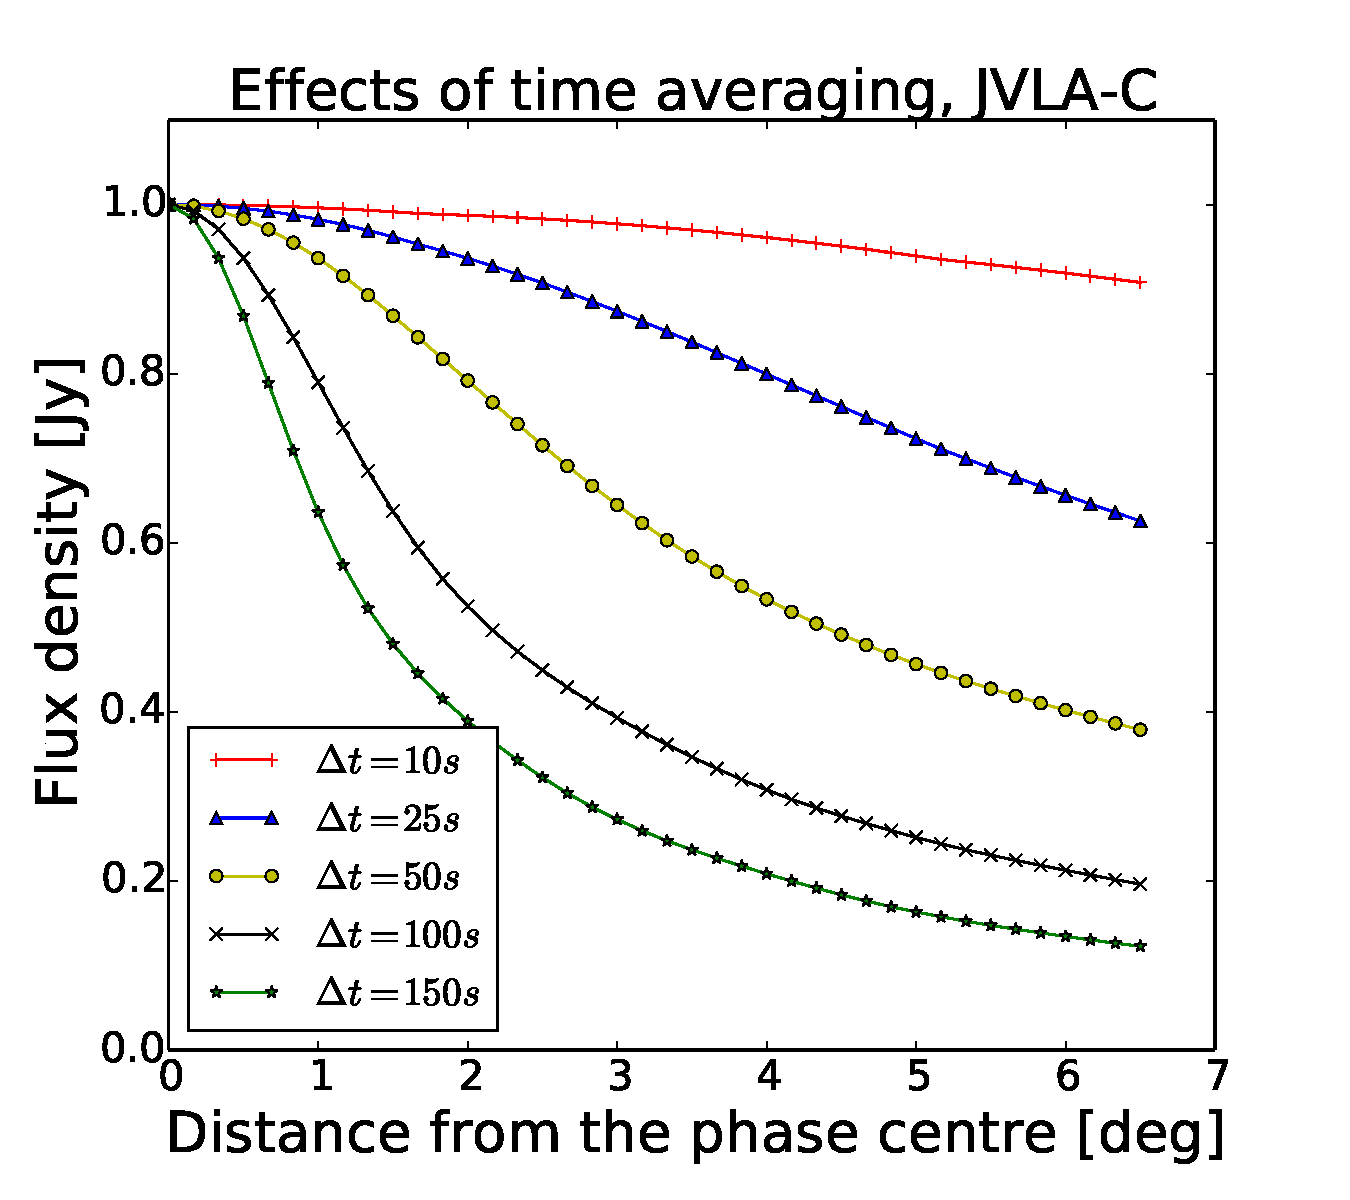
\includegraphics[width=\columnwidth]{./Figures/effect_time_averaging.pdf}%
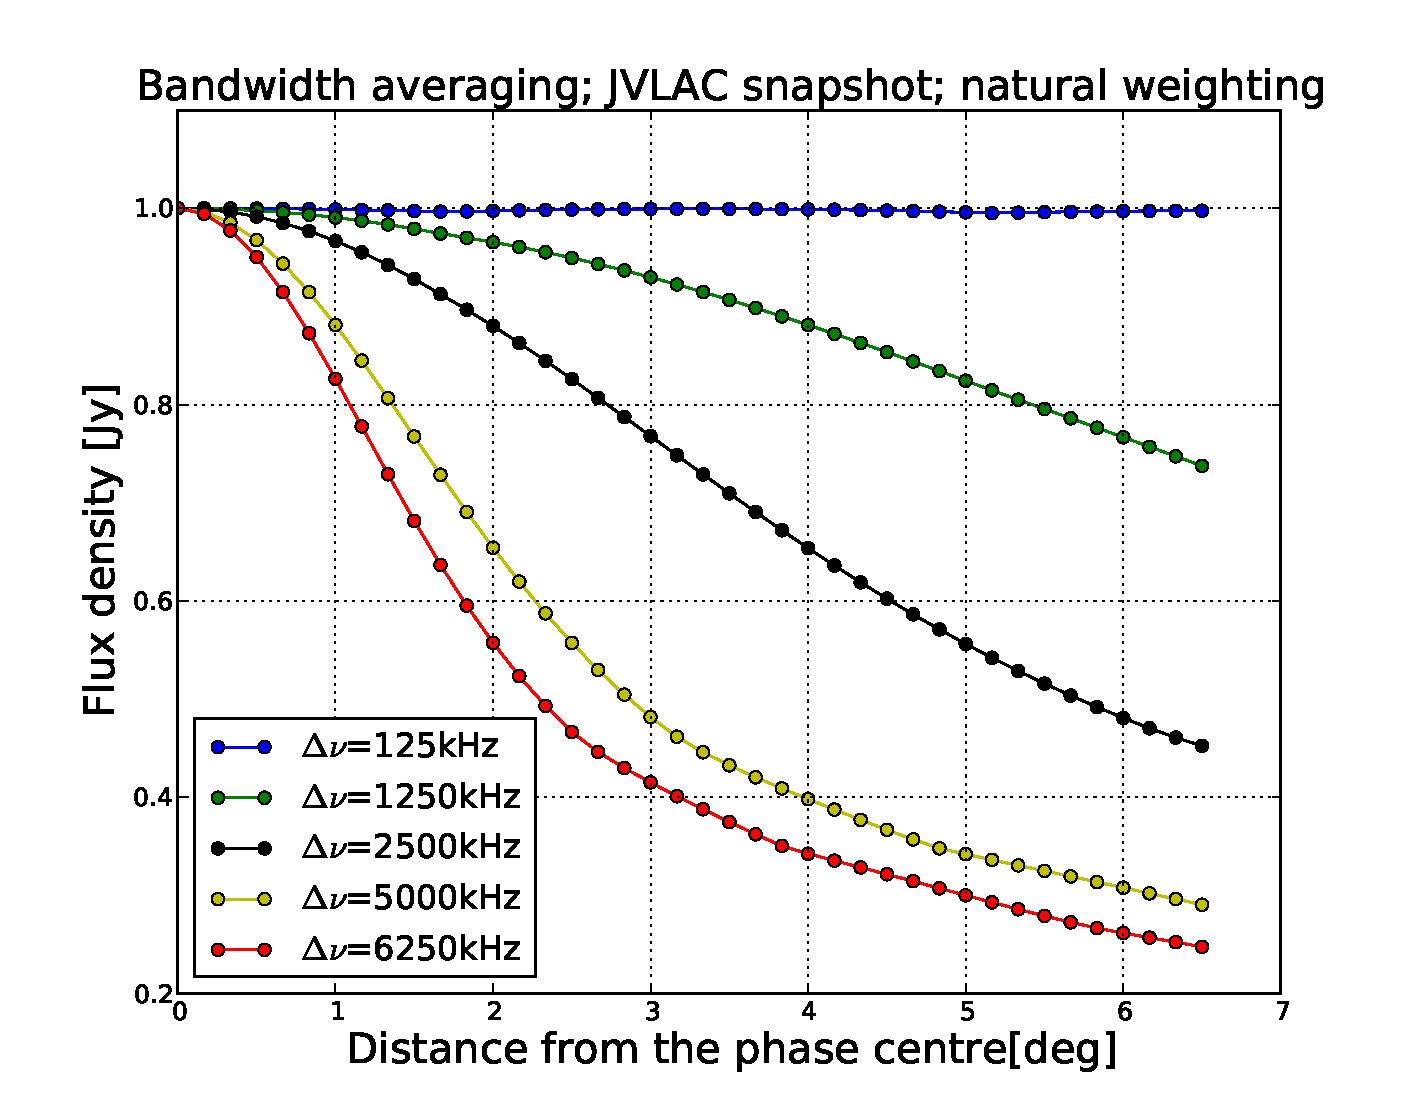
\includegraphics[width=\columnwidth]{./Figures/effect_bandwid_averaging.pdf}
\caption{Effects of time and frewuency averaging: the apparent intensity of a 1 Jy source, as seen by JVLA-C at 1.4 GHz, 
as a function of distance from phase centre. (Left) Frequency interval fixed at 125 kHz, time interval varies; 
(right) time interval fixed at 1s, frequency interval varies.}\label{fig:smear}
\end{figure*}


In the limit of $\Delta t,\Delta \nu \rightarrow 0$, averaging becomes equivalent to sampling. 
The problem arises with wide fields, because an interferometer must intrinsically use a non-zero
averaging interval. The Fourier phase component $2\pi\phi(u,v,w)$ is a function of frequency
and time, with increasing variation over the averaging interval for sources far from the phase centre.
This causes the averaging to effectively ``wash out'' source amplitude 
\citep[for an extensive discussion, see][]{bregman2012system}.

Figure \ref{fig:smear} shows the attenuation of a 1 Jy source as a function of distance
from phase centre, for a set of different time and frequency intervals. The simulations correspond to JVLA 
in the C configuration, with an observing frequency of 1.4 GHz. At this frequency, the first null of the PB is at 
$r\approx36'$, and the half-power point is at $\sim16'$, thus we can consider the ``conventional'' FoV (i.e. the half-power 
beam width, or HPBW) to be about $0.5^\circ$ across. Note that the sensitivity of the upgraded JVLA, as well as
improvements in calibration techniques \cite{Perley2013}, allow imaging to be done in the first PB sidelobe as well
(and in fact it may be necessary for deep pointings, if only to deconvolve and subtratc sidelobe sources), so we could also
consider an ``extended'' FoV extending out to the second null of the PB at $r\approx1.25^\circ$. Whatever definition
of the FoV we adopt, Fig.~\ref{fig:smear} shows that to keep amplitude losses across
the FoV to within some acceptable threshold, say 1\%, the averaging interval must be no more than some critical size,
say 10s and 1 MHz. Conversely, if we were to adopt an aggressive averaging strategy for the purposes of data 
compression, say 50s and 5 MHz, the curves indicate that we would suffer substantial amplitude loss towards the 
egde of the FoV. Finally, note that the curves corresponding to low values of smearing across the FoV (i.e. up to 25s and 
up to 1.25 MHz) have a very gentle slope, with correspondingly little suppression of sources \emph{outside} the FoV.


\subsection{Imaging and noise estimate}
\label{sec:imaging}
Recall from the previous section that, the boxcar WF can be replaced by a BDWF, $W_{pq,(t,\nu)}$ that depends 
on $(u,v)$ distances. Now, consider that $\mathcal{\textbf{W}}_{pq,(t,\nu)}$ is  $n_t \times n_{\nu}$ matrix of elements 
$W_{pq,(t_i,\nu_j)}\Big|_{i=1,n_t}^{j=1, n_{\nu}}$, the weights of uv-bins. A uv-bin is a set of four Stocks elements (XX, XY YX, YY) each 
with the same weight $W_{pq,(t_i,\nu_j)}$. Therefore, the sampled visibilities can be presented mathematically as a $4\times n_t\times 
n_{\nu}$ matrix of four polarization times and frequencies dependent matrices each of size $n_t\times n_{\nu}$.
\begin{eqnarray*}
\mathbf{V}_{pq,(t,\nu)}^{samp,i}&=&\Bigg(\mathbf{V}_{pq,(t,\nu)}^{0},\mathbf { V } 
^1_{pq,(t,\nu)},\mathbf{V}^2_{pq,(t,\nu)},\mathbf{V}_{pq,(t,\nu)}^{3 } \Bigg)^{\dagger}, \label{eqx:conv}
\end{eqnarray*}
where the symbol $^{\dagger}$ stand for the transpose operation. The convolution operator is linear, therefore we can re-write Eq.\ref{f4} 
in terms of a series of linear transformations or functional models as:
\begin{equation}
V_{pq,(t_c,\nu_c)}^{corr}= \mathbf{C}_{pq,(t,\nu)}^{block}\cdot\mathbf{W}_{pq,(t,\nu)}^{block}\cdot 
\mathbf{V}_{pq,(t,\nu)}^{samp,i}.\label{eqbb:linear}
\end{equation}
Here, $\mathbf{C}_{pq,(t,\nu)}^{block}$ and $\mathbf{W}_{pq,(t,\nu)}^{block}$ are  blocks diagonals matrices of size $(4n_t 
n_{\nu})\times(4n_t n_{\nu})$, the block elements are $\mathcal{\textbf{W}}_{pq,(t,\nu)}$ and $\mathbf{C}_{pq,(t,\nu)}$ 
respectively, where $\mathbf{C}_{pq,(t,\nu)}$ is the centre time and frequency interval sampling matrix of size $n_t\times 
n_{\nu}$. This
is the result of one time and frequency integration.
For a synthesis, the baseline (p,q) made a complete  coverage in the $(u,v)$ plane. Therefore, we can  
package into a single matrix, $\mathbf{V}_{pq,(t',\nu')}^{corr}$ of size $(4N_t N_{\nu})\times (4N_t N_{\nu})$ the 
BDWF average visibilities of the  baseline (p,q) during the synthesis as follows: 
\begin{equation}
\mathbf{V}_{pq,(t',\nu')}^{corr}=\mathbf{C}_{pq,(t,\nu)}^{block,n_{block}}\cdot 
\mathbf{W}_{pq,(t,\nu)}^{block,n_{block}}\cdot\mathbf{V}_{pq,(t,\nu)}^{samp,n_{block}}.\label{eq2:block}
\end{equation}
The size of 
$\mathbf{V}_{pq,(t',\nu')}^{corr}$ can also be written as $(4N_v^{pq})\times (4N_v^{pq})$, where $N_v^{pq}$ is the total
number of time and frequency visibilities (bins) for the baseline (p,q). The matrices
$\mathbf{C}_{pq,(t,\nu)}^{block,n_{block}}$ and $\mathbf{W}_{pq,(t,\nu)}^{block,n_{block}}$ are diagonals blocks 
matrices of size $(4N_v^{pq}n_t n_{\nu})\times (4N_v^{pq}n_t n_{\nu})$ where each diagonal block is the block diagonal matrix  
$\mathbf{C}_{pq,(t,\nu)}^{block}$ and $\mathbf{W}_{pq,(t,\nu)}^{block}$ respectively. The number of block elements is $n_{block}$. The 
sampled  visibilities 
$\textbf{V}_{pq,(t,\nu)}^{samp,n_{block}}=\mathcal{\textbf{S}}_{pq,(t,\nu)}^{n_{block}}\cdot\mathbf{V}_{pq,(t,\nu)}^{n_{block}}$ is a one 
row matrix of size 
$(N_v^{pq}4 n_t n_{\nu})\times (4 n_t n_{\nu})$ made of $\textbf{V}_{pq,(t,\nu)}^{samp,i}$ on top of each other and the matrix 
$\mathcal{\textbf{S}}_{pq,(t,\nu)}^{n_{block}}$ is the sampling function for the visibilities $\mathbf{V}_{pq,(t,\nu)}^{n_{block}}$ of 
size $(N_v^{pq}4 n_t n_{\nu})\times (4 n_t n_{\nu})$. Note that $i=1,\dots, N_v^{pq}$ and we can write:
\begin{equation}
\mathbf{V}_{pq,(t' \nu')}^{corr}= 
\mathbf{C}_{pq,(t,\nu)}^{block,n_{block}}\cdot\mathbf{W}_{pq,(t,\nu)}^{block,n_{block}}\cdot 
\mathbf{S}_{pq,(t,\nu)}^{n_{block}}\mathbf{F}\cdot\mathcal{I}_{l,m}^{sky }+\epsilon_{pq},\label{eqv:linear}
\end{equation}
our data is always corrupted by a random error component or noise, $\epsilon_{pq}$ (the error component of the baseline (p,q)).
If the number of pixel in the sky model is $N_{pix}$, then the true sky image vector $\mathcal{I}_{l,m}^{sky}$ has a size of $4N_{pix}$ and 
$\textbf{F}$ is a block diagonal Fourier transform operator of size $(4N_{pix})\times(4N_{pix})$.

We are generally interested in using the total set of visibilities over baselines, time and frequencies, having $4\times N_v$ visibilities 
measured over all baselines with $N_v=N_{bl}\times N_v^{pq}$ where $N_{bl}$ is the number of baseline. We then have:\\
\begin{equation}
 \mathbf{V}_{array,(t',\nu')}^{corr}=\mathbf{A}\cdot\mathcal{I}_{l,m}^{sky} + \epsilon. \label{eq:vall}
\end{equation}
 Here, $\epsilon$ is the array error component. $\mathbf{A}$ is a \textit{design} matrix of size 
$(4N_v)\times (4N_{pix})$ designed from $\mathbf{C}_{pq,(t,\nu)}^{block,n_{block}}\cdot \mathbf{W}_{pq,(t,\nu)}^{block,n_{block}}\cdot 
\mathbf{S}_{pq,(t,\nu)}^{n_{block}}\cdot\mathbf{F}\Big|_{p=0,\cdots,n_{a}-1}^{q=p+1,\cdots,n_{a}-1}$ on top of each order, with $n_a$ the 
number of antenna. The \textit{design} matrix is defined as:
\begin{equation*}
\mathbf{A}_{}=
  \begin{bmatrix}
    \mathbf{C}_{01,(t,\nu)}^{block,n_{block}}\cdot \mathbf{W}_{01,(t,\nu)}^{block,n_{block}}\cdot \mathbf{S}_{01,(t,\nu)}^{n_{block}} 
\cdot\mathbf{F}\\
    \vdots\\
    \mathbf{C}_{ik,(t,\nu)}^{block,n_{block}}\cdot \mathbf{W}_{ik,(t,\nu)}^{block,n_{block}}\cdot \mathbf{S}_{ik,(t,\nu)}^{n_{block}} 
\cdot\mathbf{F}\\
    \vdots \\
    \mathbf{C}_{jl,(t,\nu)}^{block,n_{block}}\cdot \mathbf{W}_{jl,(t,\nu)}^{block,n_{block}}\cdot \mathbf{S}_{jl,(t,\nu)}^{n} 
\cdot\mathbf{F}\\
  \end{bmatrix}
\end{equation*}
The dirty image, $\mathcal{I}_{l,m}^{D}$ of size $4N_{pix}$ can then be derived as follow:
\begin{equation}
\mathcal{I}_{l,m}^{D}=\bigg(\mathbf{F}^{H}\cdot\mathbf{A}\cdot\mathcal{I}^{sky}\bigg)_{(l,m)} + \epsilon.
\end{equation}
Here, $H$ represents the the conjugate transpose operation also known as a Hermitian transpose and $\mathbf{F}^{H}$ is a block diagonal
inverse Fourier transform operator of size $(4N_{pix})\times(4N_{pix})$.

The estimate of  $\epsilon$, for the map centre pixel is given by:
\begin{eqnarray}
 \widetilde{\epsilon}_{o,o}&=&\widetilde{\mathcal{I}}_{o,o} - 
\Big(\mathbf{F}^{H}\cdot\mathbf{A}\cdot\widetilde{\mathcal{I}}\Big)_{(o,o)}\\							
		      %&=&\bigg(1-\Big(\mathbf{F}^{H}\cdot\mathbf{A}\Big)_{(o,o)}\bigg)\widetilde{\mathcal{I}}_{o,o}\\		
&=&\frac{1}{N_{v}}\bigg(1-\Big(\mathbf{F}^{H}\cdot\mathbf{A}\Big)_{(o,o)}\bigg)\bigg(\mathbf{B}^{\dagger}\cdot\mathbf{V}_{array,(t,
\nu)}^{ samp } \bigg)\label{eq:noise1}.
\end{eqnarray}
Here, $\mathbf{B}$ and $\mathbf{V}_{array,(t,\nu)}^{samp}$ are  one row matrix of size $(N_v 4 n_t n_{\nu})\times (4 n_t n_{\nu})$ made of 
$\mathbf{C}_{pq,(t,\nu)}^{block,n_{block}}\cdot \mathbf{W}_{pq,(t,\nu)}^{block,n_{block}}\Big|_{p=0,\cdots,n_{a}-1}^{q=p+1,\cdots,n_{a}-1}$ 
on 
top of each other and $\mathbf{V}_{pq,(t,\nu)}^{samp,n_{block}}\Big|_{p=0,\cdots,n_{a}-1}^{q=p+1,\cdots,n_{a}-1}$ on top of each other 
respectively (see appendix \ref{app:complexmatrices} for the derivation of these complex matrices). For a noisy sky model, 
$\mathbf{V}_{array,(t, \nu)}^{ samp } =\sigma_{}\mathbf{G}$, 
where $\sigma_{}$ is the expected rms noise per visibility before boxcar averaging or BDWF averaging and $\mathbf{G}$ is a $(N_v 4 n_t 
n_{\nu}) \times (4 n_t n_{\nu})$ unit matrix. Eq.\ref{eq:noise1} can therefore be rewritten as:
\begin{eqnarray}
 \widetilde{\epsilon}_{o,o}		
&=&\frac{\sigma_{}}{N_{v}}\bigg(1-\Big(\mathbf{F}^{H}\cdot\mathbf{A}\Big)_{(o,o)}\bigg)\bigg(\mathbf{B}^{\dagger}\cdot\mathbf{G}
\bigg).\label{eq:noise}
\end{eqnarray}
The formalism of Eq.\ref{eq:noise} will be used to derive the noise estimate in section \ref{subsec:noise}.
\section{FoV signals recovery and out field suppression}
\subsection{FoV signals recovery: description and method}
\label{baseline1}
Missing spaces between sampled $(u,v)$ coordinates have an important dependence on the baseline length. However, the spacings between 
longer 
baselines $(u,v)$ coordinates are wider than the one on shorter baselines, this is the obvious effect that explained why sources are more 
distorted on longer baselines compared to shorter ones. Therefore, if one has to attribute the weight of a uv-bin, it may be proportional 
to 
the baseline length, in such a way that the distortion rate is taken into account over baselines. The study in this section aims to 
describe an approach that used a WF to assign a proper weight of a uv-bin considering the \textit{spacing} between the baseline uv-bins and 
the centre uv-bin.

Figure \ref{fig:uvcov} shows a snapshot coverage of an integration time interval. For shorter baselines, the tracks are closer to the 
centre 
of 
rotation and for longer baselines the tracks are farther away from the centre. The \textit{dot marks} are the uv-bins, 
and the  arrows indicate the separation between uv-bins and the centre uv-bin. It is trivial to see on this 
figure that these separations are wider on longer baselines. The results of boxcar averaging or BDWF averaging are assigned to the centre 
uv-bin coloured in red.

During integration, the Earth rotation makes baselines coordinates  to vary in time and 
frequency. We can therefore package the $(u,v)$ coordinates changes and the frequency changes of a baseline (p,q) into a matrix of 
size $n_t \times 2$ and  vector of dimension $n_{\nu}$ respectively. 
\begin{eqnarray*}
\mathbf{U}_{pq,t}&=& \Bigg(\mathbf{u}_{pq,t_s}, \dots , \mathbf{u}_{pq,t_c}, \dots, \mathbf{u}_{pq,t_e}\Bigg)^{\dagger}\\
 \mbox{\boldmath $\nu$}&=&\Bigg(\nu_s,\dots,\nu_c,\dots,\nu_e\Bigg)^{\dagger}.
\end{eqnarray*}
%where the indexes $s$, $c$ and $e$ depict the integration interval starting, centre and ending time respectively. 
The 
elements of $\mathbf{U}_{pq,t}$ are functions of time and frequency representing the $(u,v)$ coordinates.
A function $\overline{\overline{\cdot}}$ on a $n_t \times 2$ matrix is defined as follow:
\begin{eqnarray}
\overline{\overline{\mathbf{U}}}_{pq,t}=\Bigg(||\mathbf{u}_{pq,t_s}||, \dots , ||\mathbf{u}_{pq,t_c}||, \dots, 
||\mathbf{u}_{pq,t_e}||\Bigg)^{\dagger},
\end{eqnarray}
where $||.||$ is the Euclidean norm.
\begin{definition}[Time direction spacing]
\label{def:1}
The vector of size $n_t$ that models the spacing between uv-bins and the centre uv-bin of a baseline (p,q) across the time 
direction is defined as:
\begin{eqnarray*}
 \mathbf{d}_{t} &=&\overline{\overline{\frac{\nu_c}{c}\cdot\Bigg\{\mathbf{U}_{pq,t}-\mathbf{H}_{pq,t} \Bigg \} }},
\end{eqnarray*}
where $c$ is the speed of the light in m/s and $\mathbf{H}_{pq,t}$ is a matrix of size $n_t \times 2$ that models the centre uv-bin,\\
$\mathbf{H}_{pq,t}= \big(\mathbf{u}_{pq,t_c}, \dots , \mathbf{u}_{pq,t_c}, \dots, \mathbf{u}_{pq,t_c}\big)^{\dagger}$.
\end{definition}
\begin{definition}[Frequency direction spacing]
\label{def:2}
The vector of size $n_{\nu}$ that models the spacing between uv-bins and the centre uv-bin of a baseline (p,q) 
across the frequency direction is defined as:
\begin{eqnarray*}
\mathbf{d}^{}_{\nu} &=&\frac{||\textbf{u}_{pq,t_c}||}{c}\cdot\Bigg\{\mbox{\boldmath 
$\nu$}-\nu_c\cdot\mathbf{g}_{\nu} \Bigg \},
\end{eqnarray*}
where  $\mathbf{g}_{\nu}$ is a $n_{\nu}\times1$ unit matrix. 
\end{definition}
\begin{definition}[Baseline dependent windowing function]
\label{def:3}
If $f_{pq}$ is a \textit{baseline dependent windowing function}, then:
\begin{eqnarray*}
 f_{pq}: \{\mathbf{\mathcal{R}},\mathbf{\mathcal{R}}\} &\rightarrow& \mathbf{\mathcal{R}}\\
                   d_{t_i},d_{\nu_j} &\mapsto& \frac{w_{t_i,\nu_j}}{\sum_{i=1}^{n_t}\sum_{j=1}^{n_{\nu}}w_{t_i,\nu_j}}.
\end{eqnarray*}
Here $d_{t_i}$ is an element of the vector $\mathbf{d}_{t}$ and $d_{\nu_j}$ is an element 
of the vector $\mathbf{d}^{}_{\nu}$.
\end{definition}
The previous approach is exact but unfortunately, we do not suppress confusion sources and we lost in 
sensitivity. Although boxcar averaging \textit{means high sensitivity}, we do need to attenuate confusion sources in such a 
way that the overall Signal to Noise Ratio (SNR) becomes higher than that of boxcar averaging. The following section describe such 
method.
\subsection{Out FoV suppression: description and method}
\label{baseline2}
In theory, WFs and signals generally extend to  infinity. Unfortunately, in practice, filtering a signal with a low pass 
filter, one need to define a cut-off interval (range of uv-bins). Therefore, if one  wants to achieve sufficiently an accurate  estimate 
of the WF ideal image plane response (IPR), one need a wide cut-off interval as far as the IPR approaches 
the ideal when the WF order increases. An overlap BDWF aims to extend the order of the BDWF in 
such a way that, we approach the ideal IPR. The only drawback of this technique is the increase in time needed for processing the 
output sample of the signals being integrate.

The weight of a uv-bin is not defined by a unique BDWF but by the 
strength of the correlation between the overall  overlapping BDWF as shown in Figure \ref{fig:corrSigVLAMxBl_overlapGdelta}. 
That said, the weight of a uv-bin becomes the summation of overlapping BDWF samples on the uv-bin normalized by the summation of the 
overall uv-bins weights within the range where the overlap samples are defined.
\begin{figure*}
\begin{minipage}{0.38\linewidth}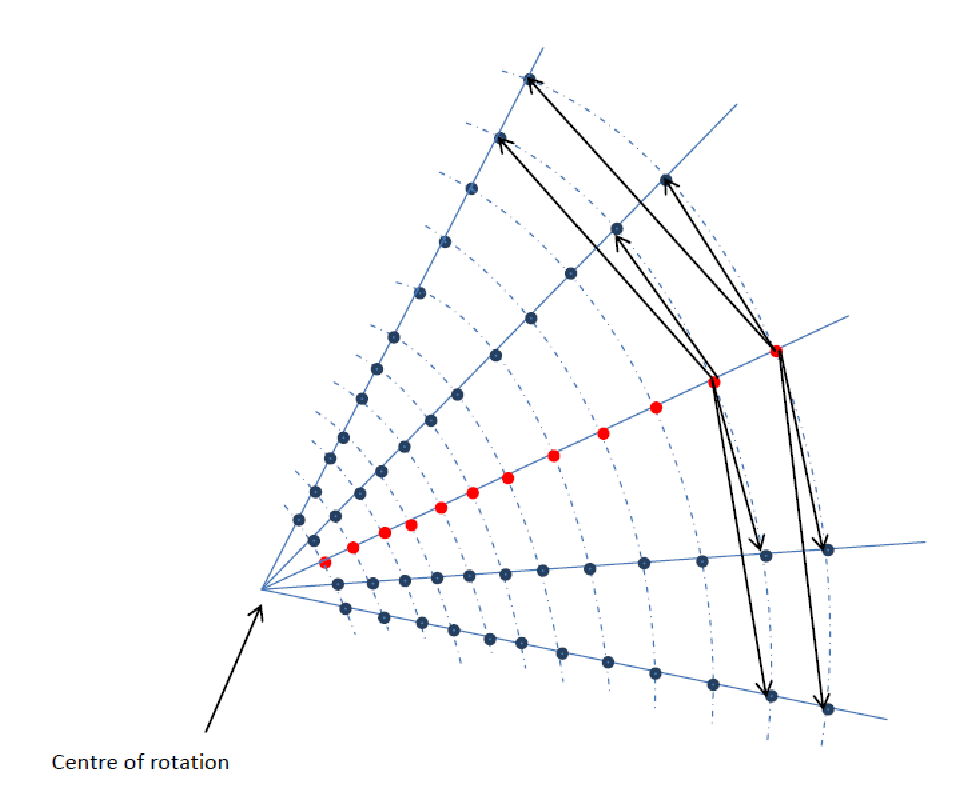
\includegraphics[width=1\textwidth]{./Figures/uvcov.png}\caption{Coverage of 
one integration}\label{fig:uvcov}\end{minipage}
  \hspace{1cm} 
\begin{minipage}{0.38\linewidth}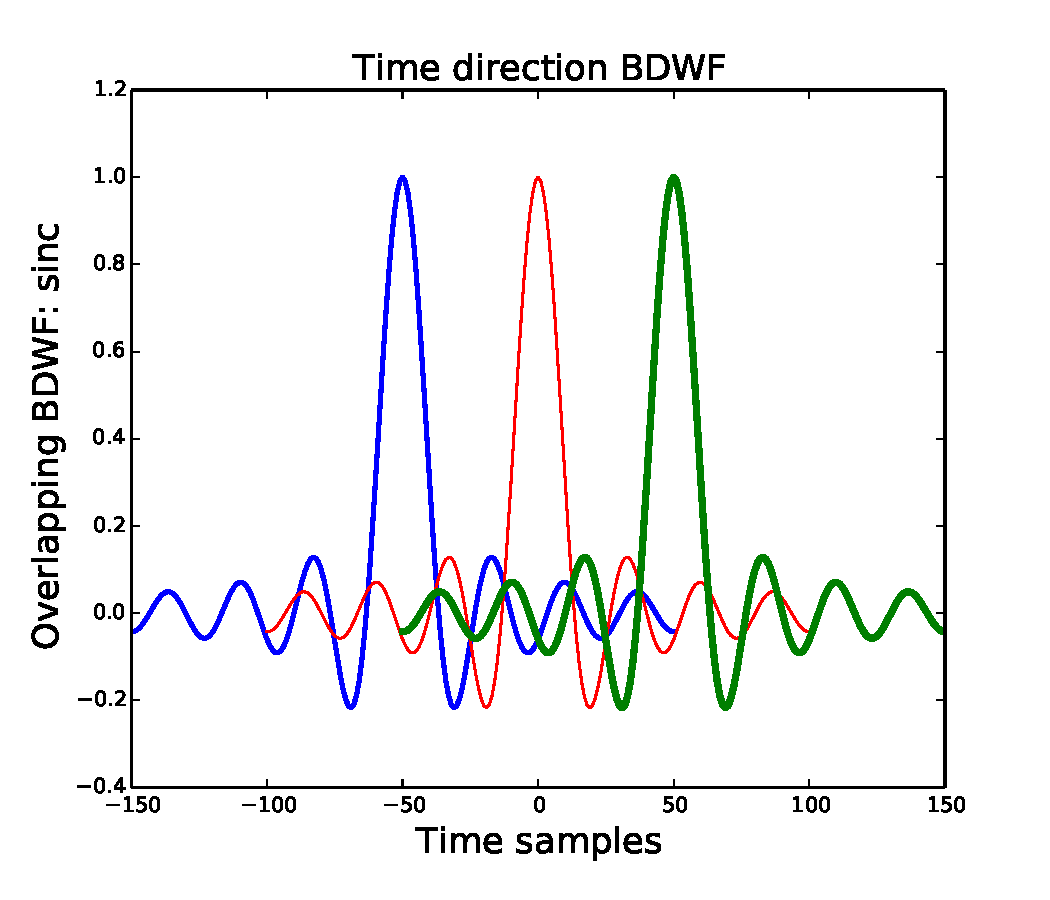
\includegraphics[width=1\textwidth]{./Figures/corrSigVLAMxBl_overlapGdelta.pdf}\caption{Overlap 
baseline dependent windowing functions}\label{fig:corrSigVLAMxBl_overlapGdelta}\end{minipage}
\end{figure*}
%Now, consider that $f^{a}_{pq}$ is an overlap-\textit{BDWF} 
%of width  $\Delta t$ and $\Delta \nu$ across the time and frequency direction respectively.
% \begin{definition}[Left hand side overlapping functions]
% \label{def:4}
% if $\Delta_l t$ and $\Delta_l \nu$ are the overlap time interval and frequency interval of the baseline dependent windowing function  
% $f_{pq}^{a_0}$ respectively  and $\Big\{f_{pq}^{a_1},f_{pq}^{a_2},f_{pq}^{a_3}, \dots \Big\}$ the set of \textit{BDWF} overlapping  on the 
% \textit{left hand side} of $f_{pq}^{a_0}$ then the resulting \textit{BDWF} within $\Delta_l t$ and $\Delta_l \nu$ is defined as
% \begin{eqnarray*}
%  g^{lhs}_{pq}: \{\mathbf{\mathcal{R}},\mathbf{\mathcal{R}}\} &\rightarrow& \mathbf{\mathcal{R}}\\
%                    d_{t_i},d_{\nu_j} &\mapsto& \frac{1}{N_{lhs}}\Bigg(\sum_{k}f_{pq,(d_{t_i},d_{\nu_j})}^{a_k} 
% + f_{pq,(d_{t_i},d_{\nu_j})}^{a_0}\Bigg).
% \end{eqnarray*}
% Here, $N_{lhs}$ is the normalization term defined as
% \begin{eqnarray*}
% N_{lhs}=\sum_{i=1}^{n_{lt}}\sum_{j=1}^{n_{l\nu}}\Bigg(\sum_{k}f_{pq,(d_{t_i},d_{\nu_j})}^{a_k} + f_{pq,(d_{t_i},d_{\nu_j})}^{a_0} \Bigg),
% \end{eqnarray*}
% where $n_{lt}$ and $n_{l\nu}$ are the number of $(u,v)$ coordinates changes and frequency changes  within $\Delta_l t$ and $\Delta_l \nu$ 
% respectively.
% \end{definition}
% \begin{definition}[Right hand side overlapping functions]
%  \label{def:4}
%  if $\Delta_r t$ and $\Delta_r \nu$ are the overlap time and frequency interval of a \textit{BDWF} $f_{pq}^{a_0}$ 
% respectively and  $\Big\{f_{pq}^{a_1},f_{pq}^{a_2},f_{pq}^{a_3}, \dots \Big\}$ the set of \textit{BDWF} overlapping on the \textit{right 
% hand side} of $f_{pq}^{a_0}$, then the 
% resulting \textit{BDWF} within $\Delta_r t$ and $\Delta_r \nu$ is defined as
% \begin{eqnarray*}
%  g^{rhs}_{pq}: \{\mathbf{\mathcal{R}},\mathbf{\mathcal{R}}\} &\rightarrow& \mathbf{\mathcal{R}}\\
%                    d_{t_i},d_{\nu_j} &\mapsto& 
% \frac{1}{N_{rhs}}\Bigg (f_{pq,(d_{t_i},d_{\nu_j})}^{a_0}+\sum_{k}f_{pq,(d_{t_i},d_{\nu_j})}^{a_k}\Bigg ).
% \end{eqnarray*}
% Here, $N_{rhs}$ is the normalization term defined as
% \begin{eqnarray*}
% N_{rhs}=\sum_{i=1}^{n_{rt}}\sum_{j=1}^{n_{r\nu}}\Bigg(f_{pq,(d_{t_i},d_{\nu_j})}^{a_0} + \sum_{k}f_{pq,(d_{t_i},d_{\nu_j})}^{a_k}\Bigg),
% \end{eqnarray*}
% where $n_{rt}$ and $n_{r\nu}$ are the number of $(u,v)$ coordinates changes and frequency changes  within $\Delta_r t$ and $\Delta_r \nu$ 
% respectively.
% \end{definition}
% \begin{definition}[Overlap baseline dependent windowing functions]
%  \label{def:4}
% If $f_{pq}^{a_0}$ is a baseline dependent windowing function defined within the time interval $\Delta t$ and the frequency interval 
% $\Delta \nu$, $g^{lhs}_{pq}$ the result of the left hand side of $f_{pq}^{a_0}$ overlapping windowing functions within the time interval 
% $\Delta_l t$ and the frequency interval $\Delta_l \nu$, and $g^{rhs}_{pq}$  the result of the right hand side of $f_{pq}^{a_0}$ overlapping 
% windowing functions within the time interval $\Delta_r t$ and the frequency interval 
% $\Delta_r \nu$, then the overlap baseline dependent windowing function within  $\Delta t$ and $\Delta \nu$ is defined as:
% \begin{eqnarray*}
%  g^{}_{pq}: \{\mathbf{\mathcal{R}},\mathbf{\mathcal{R}}\} &\rightarrow& \mathbf{\mathcal{R}}\\
%                    d_{t_i},d_{\nu_j} &\mapsto&
%  \left\{ 
%   \begin{array}{l l}
%     g^{lhs}_{pq} & \quad \text{if $(t_i,\nu_j) \in (\Delta_l t, \Delta_l \nu)$}\\
%     f^{a_0}_{pq} & \quad \text{if $(t_i,\nu_j) \in (\Delta_m t, \Delta_m \nu)$}\\
%     g^{rhs}_{pq}& \quad \text{if $(t_i,\nu_j) \in (\Delta_r t, \Delta_r \nu)$}
%   \end{array} \right.
% \end{eqnarray*}
% \end{definition}
% where $\Delta_m t$ and $\Delta_m \nu$ are $f_{pq}^{a_0}$ uncorrelated time  and frequency interval respectively. From the above 
% definitions, the following derivation is trivial 
% \begin{equation*}
%  \Big\{\Delta t,\hspace{0.17cm}\Delta \nu \Big\}=\Big\{\Delta_l t \cup \Delta_m t \cup \Delta_r t, \hspace{0.17cm}\Delta_l \nu \cup 
% \Delta_m \nu \cup \Delta_r \nu \Big\}.
% \end{equation*}
%  They follow the rules below:
% \begin{eqnarray*}
%  \Delta_m t= \left\{ 
%   \begin{array}{l l}
%      \cup\{t_i\}_{i=s',\hspace{0.1cm} s' \geq s+1}^{e', \hspace{0.1cm}e'\leq e-1} & \quad \text{if $n_{lt}+n_{rt}< n_t$}\\
%       \{t_c\}& \quad \text{if $n_{lt}+n_{rt} = n_t$}\\
%        \emptyset  & \quad \text{otherwise}
%   \end{array} \right.
% \end{eqnarray*}
% and
% \begin{eqnarray*}
%  \Delta_m \nu= \left\{ 
%   \begin{array}{l l}
%      \cup\{\nu_i\}_{i=s',\hspace{0.1cm} s'\geq s+1}^{e', \hspace{0.1cm}e'\leq e-1} & \quad \text{if $n_{l\nu}+n_{r\nu} < n_{\nu}$}\\
%       \{\nu_c\}& \quad \text{if $n_{l\nu}+n_{r\nu} = n_{\nu}$}\\
%        \emptyset  & \quad \text{otherwise}
%   \end{array} \right.
% \end{eqnarray*}
\section{Analysis of windowing functions}
\label{subsec:Windowing functions}
In signal processing a WF is a mathematical function that has zero-values outside some chosen interval, and when a signal 
is multiplied by the WF, the product has also zero-values outside the interval.
In this section, we evaluated the Peak Sidelobe Level (PSL), the Main 
Lobe width (MLW) and the Sidelobes Roll-off (SLR) for some WFs. Allowing this paper to be useful both in signal processing and radio 
astronomy community, the terminology that is used in radio astronomy in contrast of the terminology used 
in signal processing is presented in the table below.\\
\\
\begin{tabular}{*3{c}}
 \multicolumn{3}{|c|}{}
 \hspace{-1cm}\begin{tabular}{|l|l|l|l|}
  \hspace{3cm}\footnotesize Table of terms \\
  \hline
  \footnotesize Signal processing &\footnotesize BDWFs\\
  \hline\hline
  {\footnotesize Frequency (freq) domain} &{\footnotesize Image plane} \\
  {\footnotesize Time domain} &{\footnotesize Fourier plane}\\
  {\footnotesize Spectral response or freq response} & {\footnotesize Image plane response}\\
   {\footnotesize Time response} & {\footnotesize Fourier plane response}\\
  {\footnotesize Cut-off time interval or time pass band} &{\footnotesize uv-bins range}\\
  {\footnotesize Cut-off freq interval or freq pass band} &{\footnotesize FoV}\\
  {\footnotesize Time stop band} &{\footnotesize Outside uv-bins range}\\
  {\footnotesize Freq stop band} &{\footnotesize Outside edges of FoV}\\
  \end{tabular}
\end{tabular}\\
\\

The goal of this section is threefold, find a WF that its IPR will:
\begin{itemize}
  \item Conserved the signal within a field of interest "\textit{Regime 1}": that said a WF with a narrower MLW.
  \item Achieved less masking of nearby sources by restricting "\textit{Regime 2}" to a narrower band: that said a WF with a lower PSL.
  \item Attenuated sidelobes confusion from far away sources "\textit{Regime 3}": that said a WF with a SLR that drops faster.
\end{itemize}
Such a WF is very common in theory, is a continuous 
function (unsampled function) over an illimitable time interval with unit area as shown in Figure \ref{fig:idealWF} and its ideal IPR in 
Figure \ref{fig:idealIRF}. 
\begin{figure*}
\begin{minipage}{0.4\linewidth}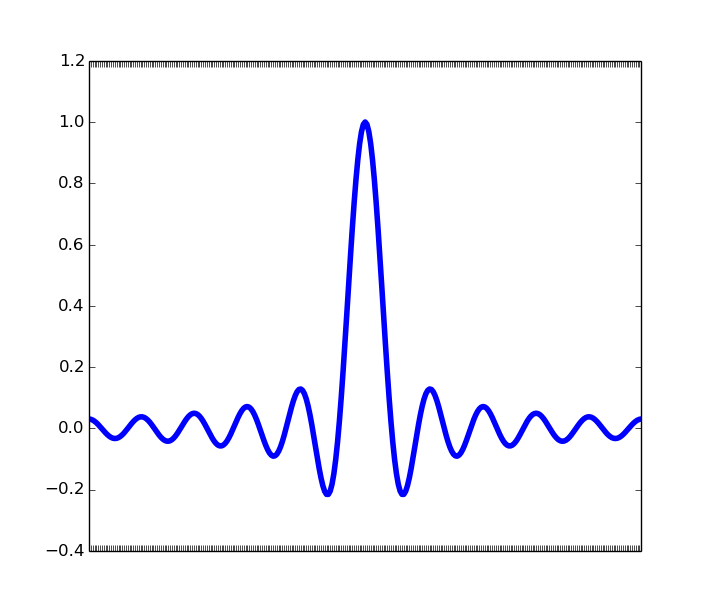
\includegraphics[width=1.1\textwidth]{./Figures/idealsinc.png}\caption{Ideal 
WF}\label{fig:idealWF}
\end{minipage}
  \hspace{1cm} 
\begin{minipage}{0.38\linewidth}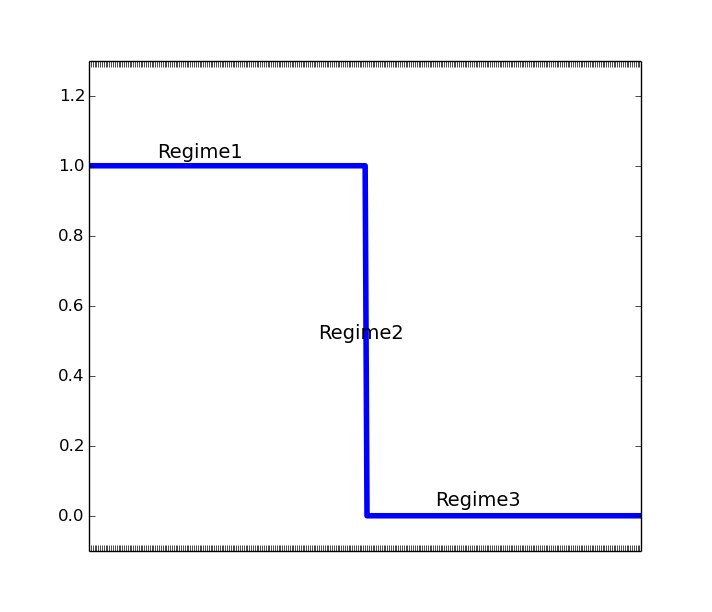
\includegraphics[width=1.\textwidth]{./Figures/idealIPR.png}\caption{Ideal 
IPR}\label{fig:idealIRF}\end{minipage}
\end{figure*}
% \begin{itemize}
%   \item Find a windowing function that its IPR will conserved the signal within a field of interest 
%   \item while suppressing sidelobes confusion from strong sources outside the field of interest.
% \end{itemize}   
\subsection{Boxcar window}
The Boxcar window is a function that  conserved a constant non-zero value  inside a chosen  interval and zero value outside this interval. 
For a cut-off time interval  $[-t_a,t_a]$ the boxcar window is defined as:
\begin{equation}
\Pi(t)=\left\{
\begin{array}{rl}
1 & \mbox{$-t_a \leq t \leq t_a$} \\
0 & \mbox{otherwise}
\end{array}\right.
\end{equation}
Figures \ref{fig:fig_box} and \ref{fig:fig_box_freq} give the graph of $\Pi(t)$ and its IPR  respectively. The blue and 
the red curves of Figure \ref{fig:fig_box_freq} are the IPRs of $\Pi(t)$ for a cut-off time interval $[-t_a, t_a]$ and 
$[-t_a/2,t_a/2]$ respectively. Note that when the cut-off time interval is large, the MLW of the IPR is 
narrower, the PSL is lower and the SLR drops faster.
\subsection{Gaussian window}
A Gaussian window centered at mean zero with standard deviation $\sigma$ is given by: 
\begin{equation}
  G(t)= e^{-bt^{2}}, \label{eq:gauss}
\end{equation}
where, $b=(2\sigma_1^2)^{-1}$. The  Fourier transform of Eq.\ref{eq:gauss} is given by 
$\mathcal{F}\big\{G(t)\big\}=\sqrt{\frac{b}{\pi}}e^{-cl^2}$, where $c=\pi^2/b$.
This shows us that the Fourier transform of a Gaussian with standard deviation $\sigma_1$ is a Gaussian with a standard 
deviation $\sigma_2= (2\pi\sigma_1)^{-1}$.
Figure \ref{fig:fig_gauss} and \ref{fig:fig_gauss_freq} give the graph of $G(t)$ and its IPR respectively, where $G(t)$ 
is truncated within the cut-off time interval $[-t_a,t_a]$, with $b = 3$ for the blue curve and $b=5$ for the red curve. Note 
that when the standard deviation is large, the MLW of the IPR is narrower, the PSL is higher and the SLR drops slowly compared to a 
smaller standard deviation.
\subsection{Butterworth window}
The time response of the Butterworth window is flat  in the time pass band, and rolls off towards zero in the time stop band and it is 
characterized by two independent parameters, the cut-off time time $[-t_a,t_a]$ and the order $p$. The two parameters control the 
FoV and sidelobes  attenuation. The time response of the Butterworth window is given by:
\begin{equation}
BW(t)= \Big(1 + (t/t_a)^{2p}\Big)^{-1}.
\end{equation}
For a same time interval $[-t_a,t_a]$, three curves of $BW(t)$ ($p=1, p=3, p=5$) are plotted  in Figure \ref{fig:fig_butter} and 
their corresponding IPRs are plotted in Figure \ref{fig:fig_butter_freq}. Note that when the order $p$ increases, the MLW of the 
IPR is conserved, while the PSL increase and the SLR drop faster.
\subsection{Sinc Window}
The sinc window is defined as follow:
\begin{equation}
S(t)= sinc\big(\pi b t\big).
\end{equation}
 Figures \ref{fig:fig_sinc} and \ref{fig:fig_sinc_freq} give the graph of $S(t)$ and its IPR respectively, where 
$S(t)$ is truncated within the time interval $[-t_a,t_a]$. Note that when the time interval is large 
(see Figure \ref{fig:fig_sinc_freq}, blue curve), the IPR becomes perfectly flat at the frequency pass band (FoV) while the MLW becomes 
narrower,  the PSL 
becomes lower and the SLR drops faster compared to a narrower time interval $[-t_a/2,t_a/2]$ (see Figure \ref{fig:fig_sinc_freq}, red 
curve). 
\subsection{Bessel Function of the First Kind of order zero}
 The function can  be determined using the infinity power series expansion:
\begin{equation}
J_0(t) = \sum_{k=0}^{\infty}\frac{(-1)^k (x/2)^{2k}}{(k!)^2}
\end{equation}
 Figures \ref{fig:bessel} and  \ref{fig:freq_resp_bessel} give the graph of J$_0(t)$ and its IPR respectively, where 
J$_0(t)$ is truncated within the time interval $[-t_a,t_a]$. Note that when the time interval is large 
(Figure \ref{fig:freq_resp_bessel}, blue curve), the IPR is flat at the frequency pass band (FoV) while the MLW becomes narrower,  the PSL 
becomes lower and the SLR drops faster compared to a narrower time interval $[-t_a/2,t_a/2]$ (Figure \ref{fig:freq_resp_bessel}, red curve).
\subsection{Convolution theorem and WFs comparison}
We begin with a continuous signal $V_{t}$ (supposed the data is only time dependent) and sample it in order to obtain the set of 
measurement (see section \ref{sec:AvgCon}). When the signal is limited in the time interval $[-t_a,t_a]$ and convolved with a window 
$W_{t}$, it 
follows from the convolution theorem that the process was equivalent to "\textit{tapering the  Fourier transform of the signal}" by 
effectively looking at the true Fourier transform of the signal through the convolution window. This is presented mathematically as:
\begin{equation}
\mathcal{F}\Big\{V_{t}\circ W_{t}\Big\} = \mathcal{F}\Big\{V_{t}\Big\}\cdot \mathcal{F}\Big\{W_{t}\Big\}
\end{equation}
One can replaced the convolution window, $W_{t}$ by its Fourier transform. A summary of the MLW, the PSL and 
the SLR of the windows study is showed in table below.

\begin{tabular}{*3{c}}
 \multicolumn{3}{|c|}{}\\
 \hspace{-1cm}\begin{tabular}{|l|l|l|l|}
  \hline
  \footnotesize $|\mathcal{F}\Big\{W_{t}\Big\}|$ &\textbf{\footnotesize MLL (-3db)}&\textbf{\footnotesize PSL (db)} &\textbf{\footnotesize 
SLR (db/octave) }  \\
  \hline\hline
  {\footnotesize $\Pi(t)$} &{\footnotesize $\approx 0,073$} &{\footnotesize $-6,68$}&{\footnotesize 
$-6,78$}\\
  {\footnotesize $S(t)$} &{\footnotesize  $\approx0,306$}&{\footnotesize  $-11,22$}&{\footnotesize  
$-12,42$} \\
  {\footnotesize $G(t)$} & {\footnotesize $\approx0,0736$}&{\footnotesize  $-30,28$}&{\footnotesize  $-14,5$}\\ 
  {\footnotesize $BW(t)$} &{\footnotesize  $\approx0,079$} &{\footnotesize $-10,08$ }&{\footnotesize  $-15,39$}\\
  {\footnotesize $J_0(t)$} &{\footnotesize  $\approx 0,39$} &{\footnotesize $ -15,01$ }&{\footnotesize  $ -14,01$}
  \end{tabular}& \label{BDWBnoise}
\end{tabular}\\
\\

\hspace{-0.6cm}The sinc, the Bessel of the first kind of order zero (J$_0$) and the Butterwordth (BW)  approach the specification of this 
research and they are taken under consideration in the rest of this paper.  We considered sinc(X,Y)=sinc(X)sinc(Y), 
J$_0$(X,Y)=J$_0(\sqrt{X^2 + Y^2})$ and BW(X,Y)=BW($\sqrt{X^2 + Y^2})$ for  two dimensional 
sinc, J$_0$ and BW respectively.
The following designations will be used in the rest of the paper:

Bl-WF-$n_{ovlpt}\times -$: One dimensional BDWF applied across the time direction; WF is one of the window under 
consideration (sinc, J$_0$ and BW) and $2n_{ovlpt}$ is the number of overlap time bins.

Bl-WF-$-\times n_{ovlp\nu}$: One dimensional BDWF applied across the frequency direction with $2n_{ovlp\nu}$ the number of overlap 
frequency bins.

Bl-WF-$n_{ovlpt}\times n_{ovlp\nu}$: Two dimensional BDWF applied across both time and frequency direction.

Bx-avg-$0\times -$: Boxcar averaging applied across the time direction.

Bx-avg-$-\times 0$: Boxcar averaging applied across the frequency direction. 

Bx-avg-$0\times 0$: Boxcar averaging applied across both time and frequency direction.
\begin{figure*}
  \centering
  \begin{minipage}{0.38\linewidth}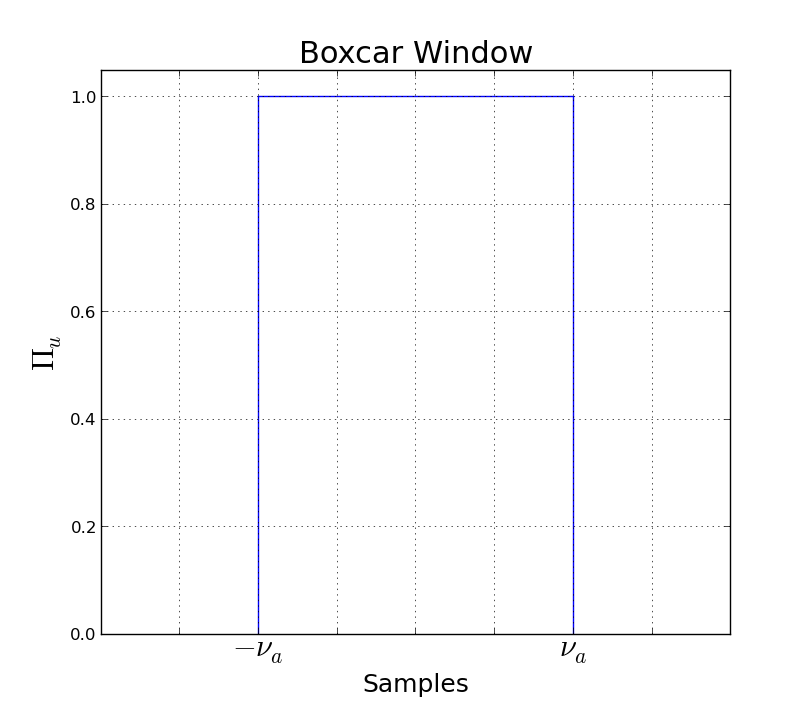
\includegraphics[width=1\textwidth]{./Figures/rect.png}\caption{Boxcar windowing 
function.}\label{fig:fig_box}\end{minipage}
\hspace{1cm}
\begin{minipage}{0.38\linewidth}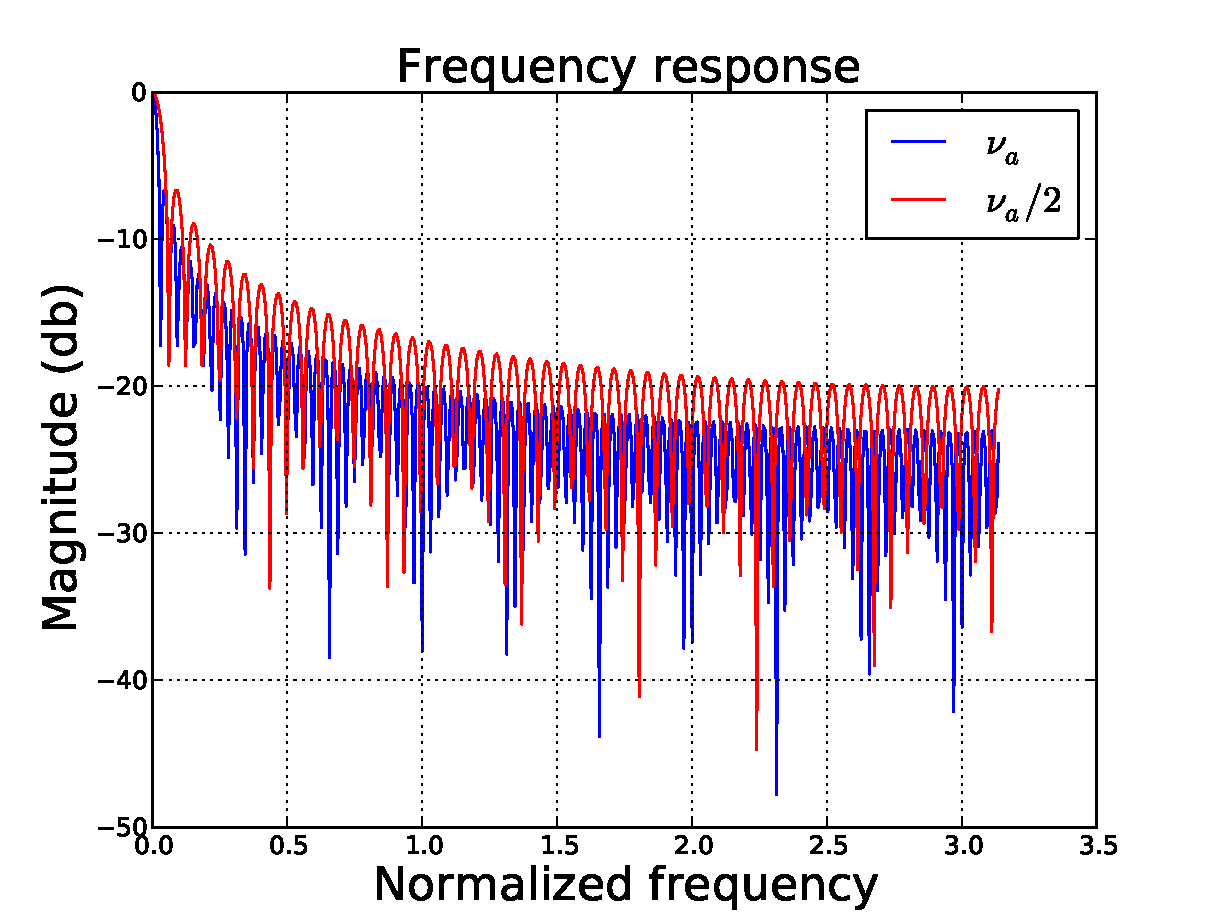
\includegraphics[width=1\textwidth]{./Figures/freq_resp_box.pdf}\caption{Frequency response of a boxcar 
window}\label{fig:fig_box_freq}\end{minipage}\\
\begin{minipage}{0.38\linewidth}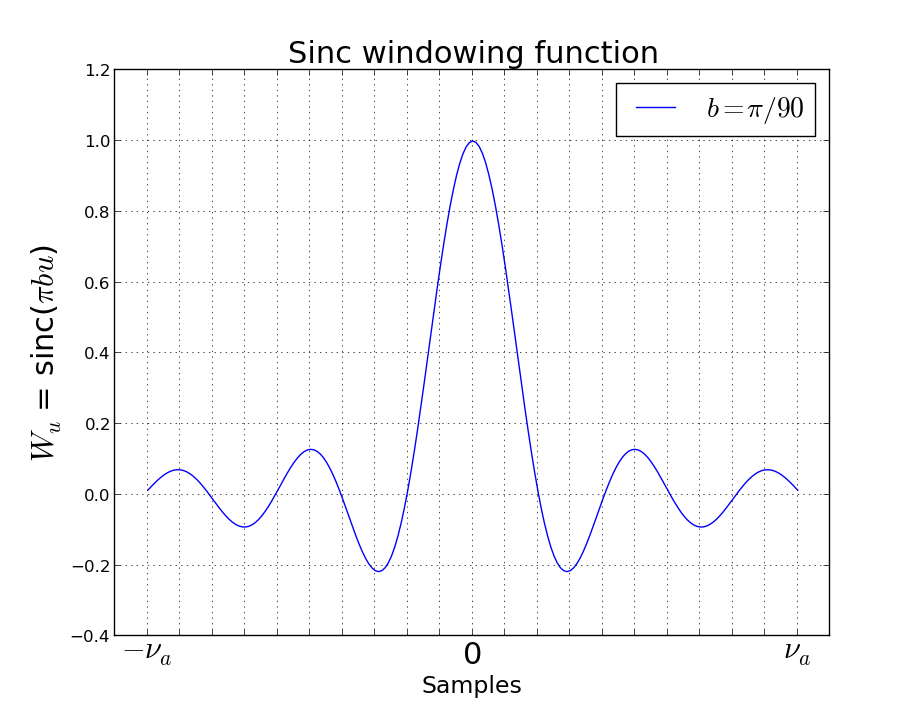
\includegraphics[width=1\textwidth]{./Figures/sinc.png}\caption{Sinc 
window}\label{fig:fig_sinc}\end{minipage}
\hspace{1cm}
\begin{minipage}{0.38\linewidth}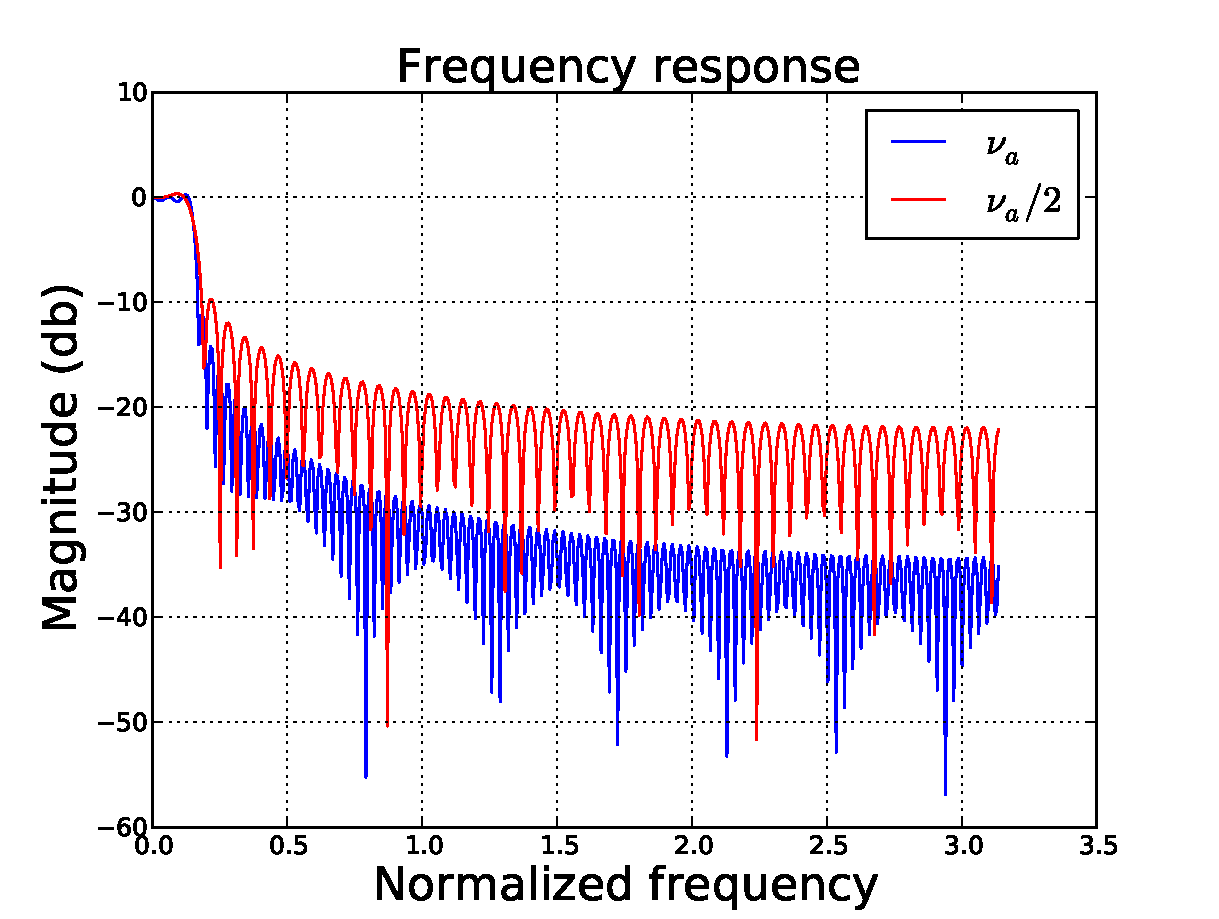
\includegraphics[width=1\textwidth]{./Figures/freq_resp_sinc.pdf}\caption{Frequency response of the 
sinc window }\label{fig:fig_sinc_freq}\end{minipage}\\
\begin{minipage}{0.38\linewidth}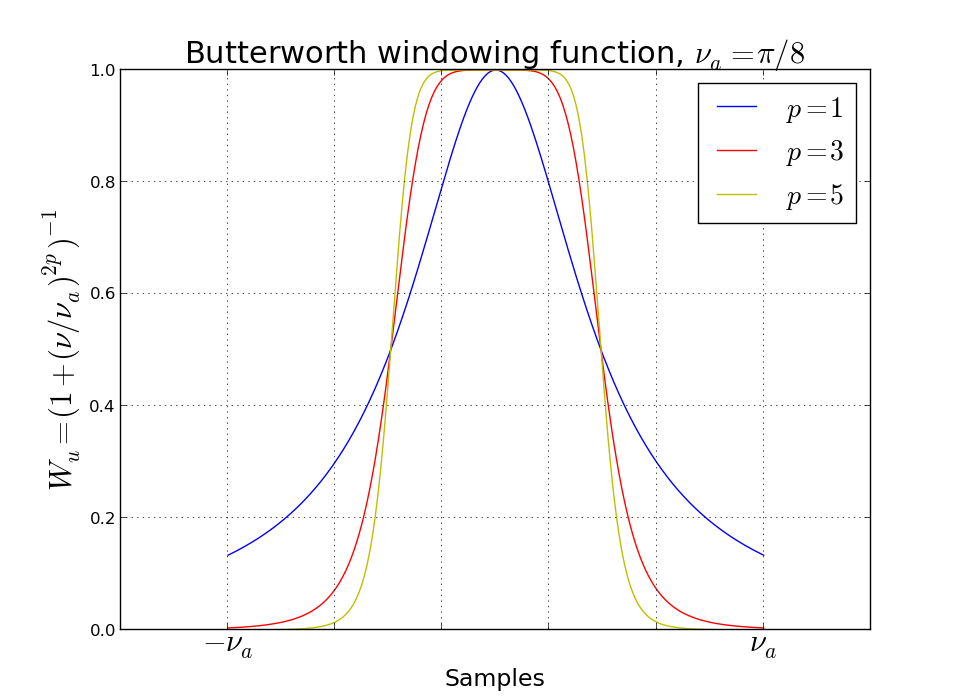
\includegraphics[width=1\textwidth]{./Figures/Butterwordth.pdf}\caption{ Butterwordth 
windows}\label{fig:fig_butter}\end{minipage}
\hspace{1cm}
\begin{minipage}{0.38\linewidth}\includegraphics[width=1\textwidth]{./Figures/freq_resp_butterwordh.pdf}\caption{Frequency response 
of the Butterwordth windows}\label{fig:fig_butter_freq}\end{minipage}\\
\begin{minipage}{0.38\linewidth}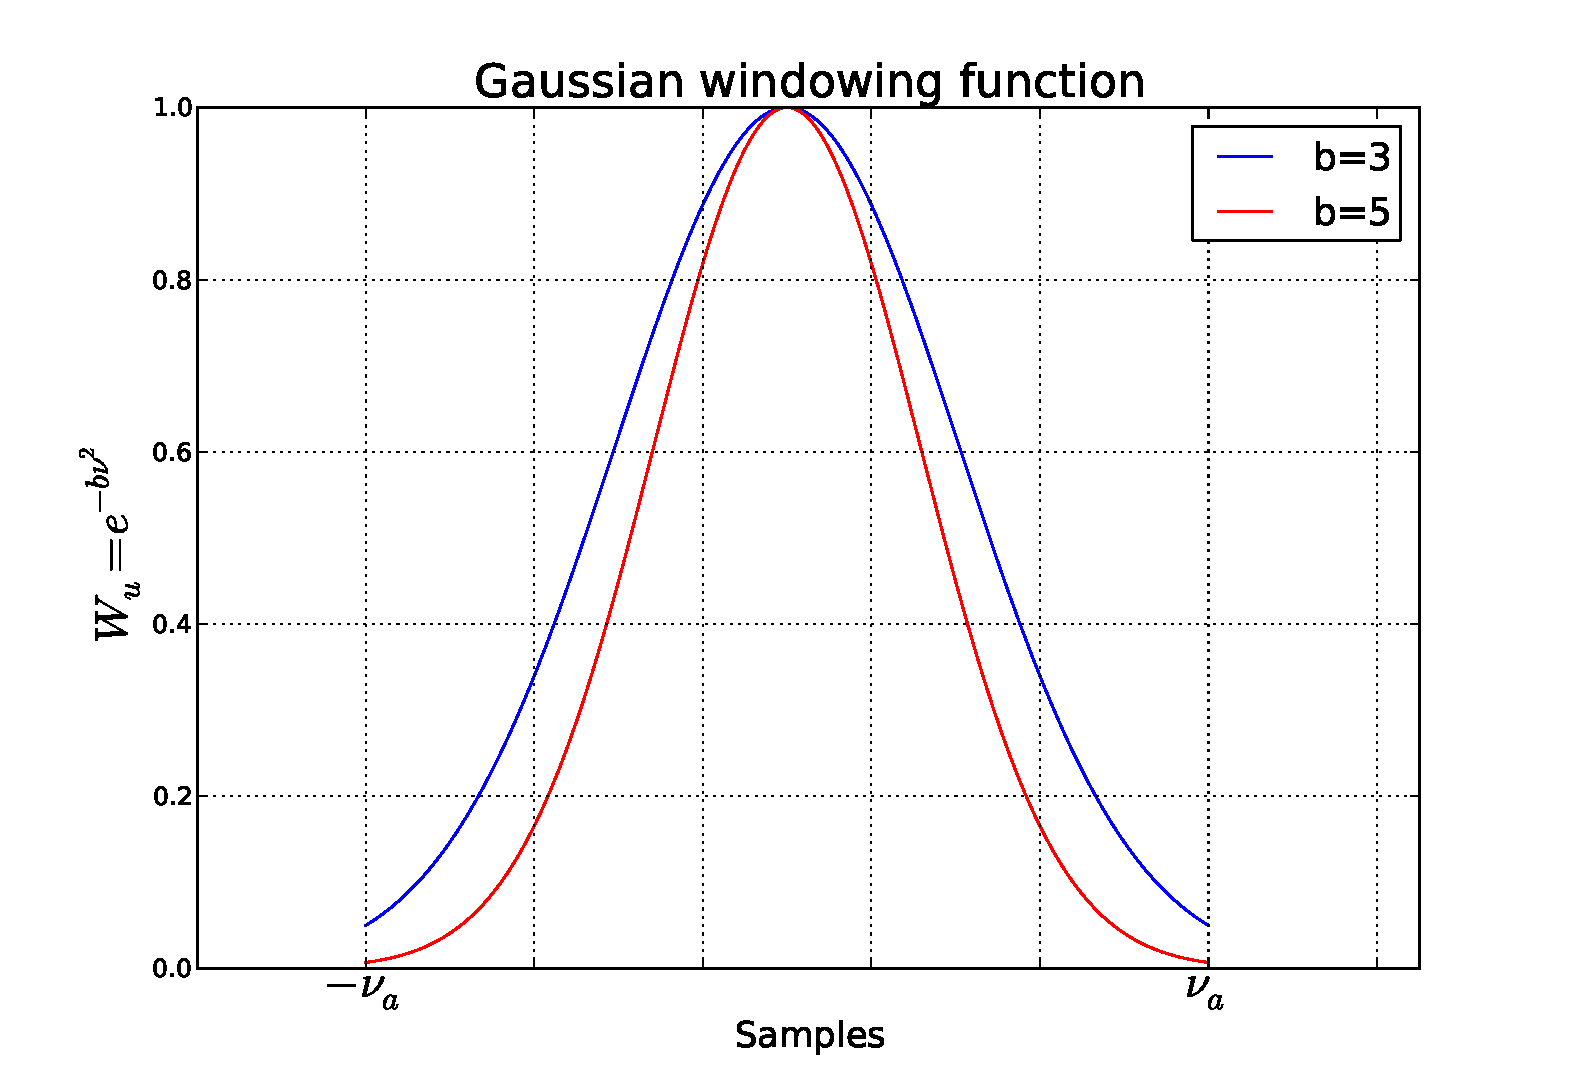
\includegraphics[width=1\textwidth]{./Figures/gausian.pdf}\caption{Gaussian windows}\label{fig:fig_gauss}
\end{minipage}
\hspace{1cm}
\begin{minipage}{0.38\linewidth}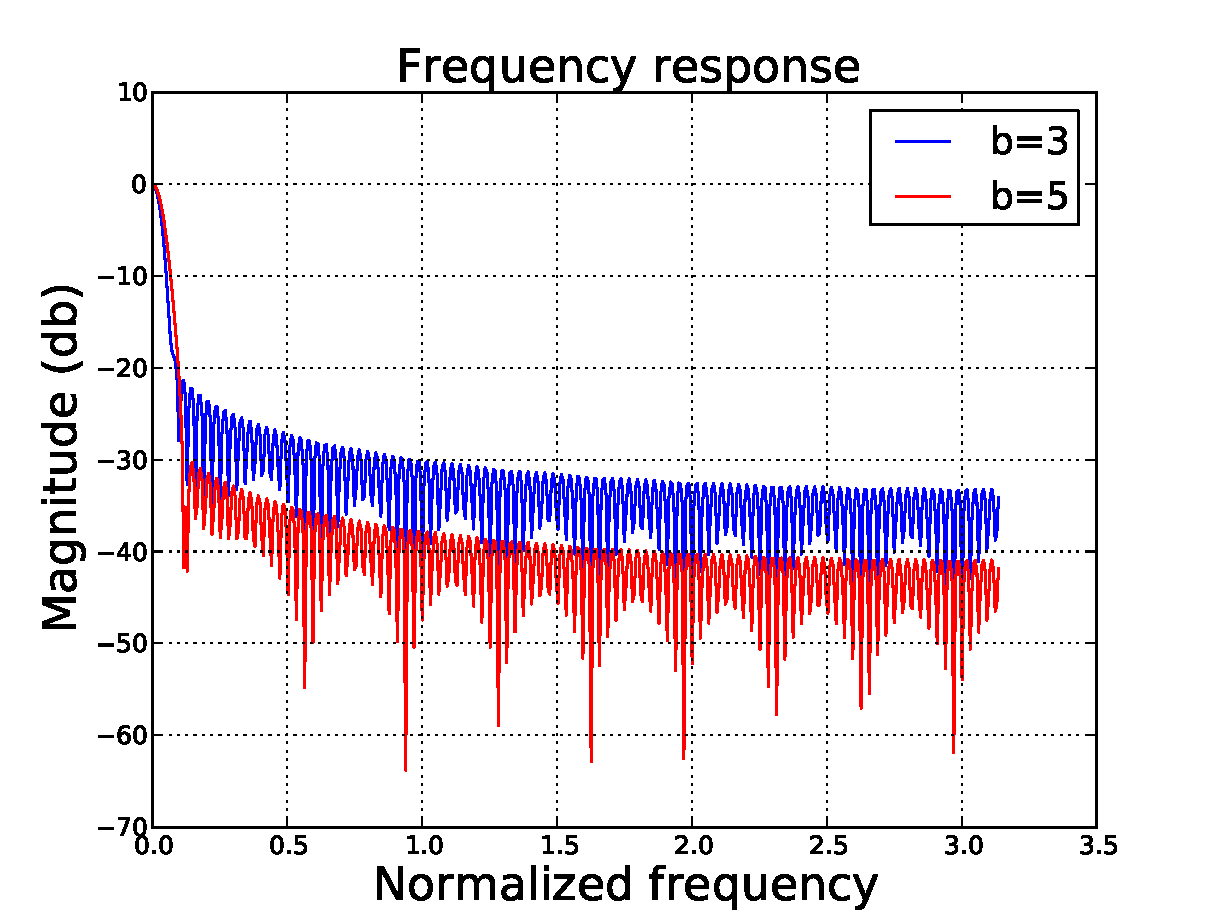
\includegraphics[width=1\textwidth]{./Figures/freq_resp_gaussian.pdf}\caption{Frequency response of 
Gaussian windows}\label{fig:fig_gauss_freq} \end{minipage}
\end{figure*}
\begin{figure*}
  \centering
\begin{minipage}{0.38\linewidth}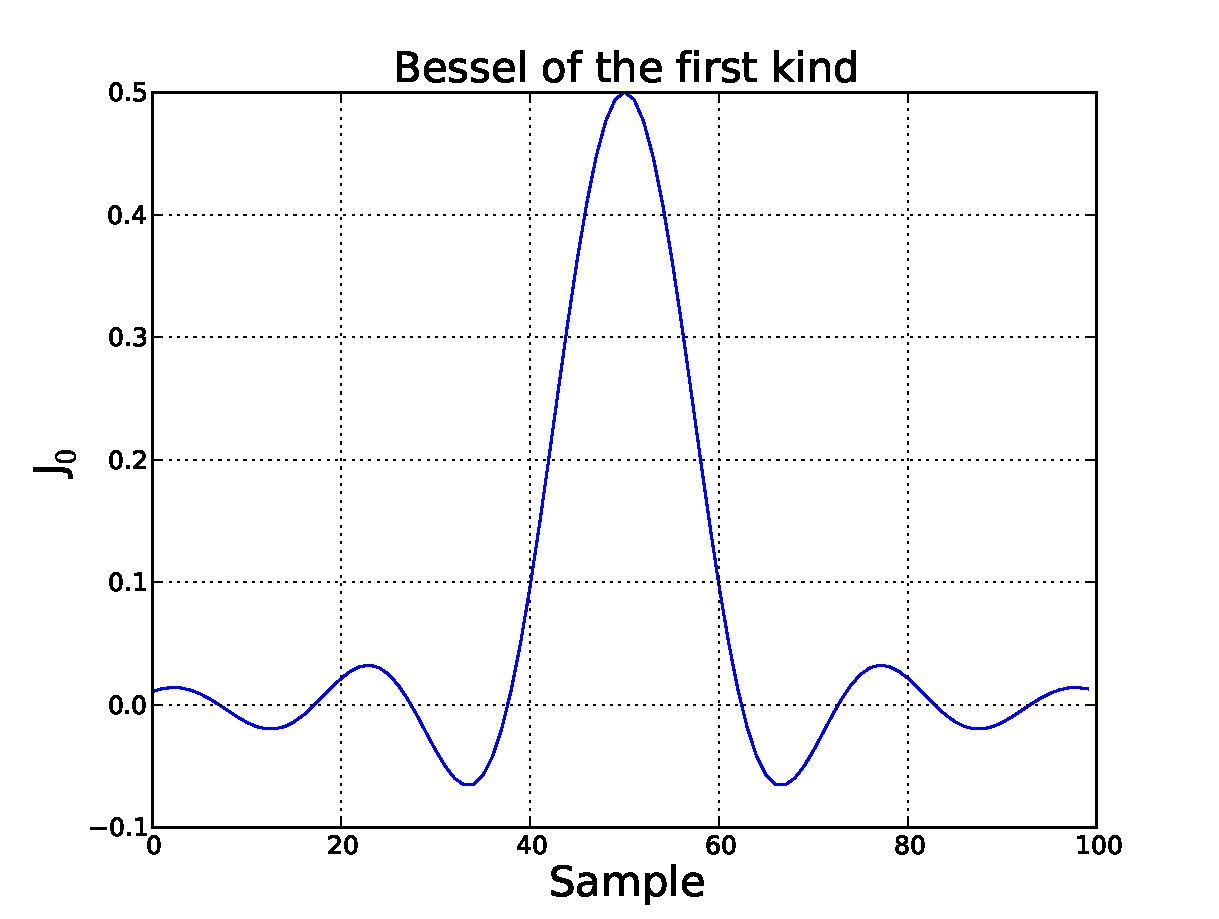
\includegraphics[width=1\textwidth]{./Figures/bessel.pdf}\caption{Bessel 
first King windows NB: this figure is coming very soon}\label{fig:bessel}\end{minipage}
\hspace{1cm}
\begin{minipage}{0.38\linewidth}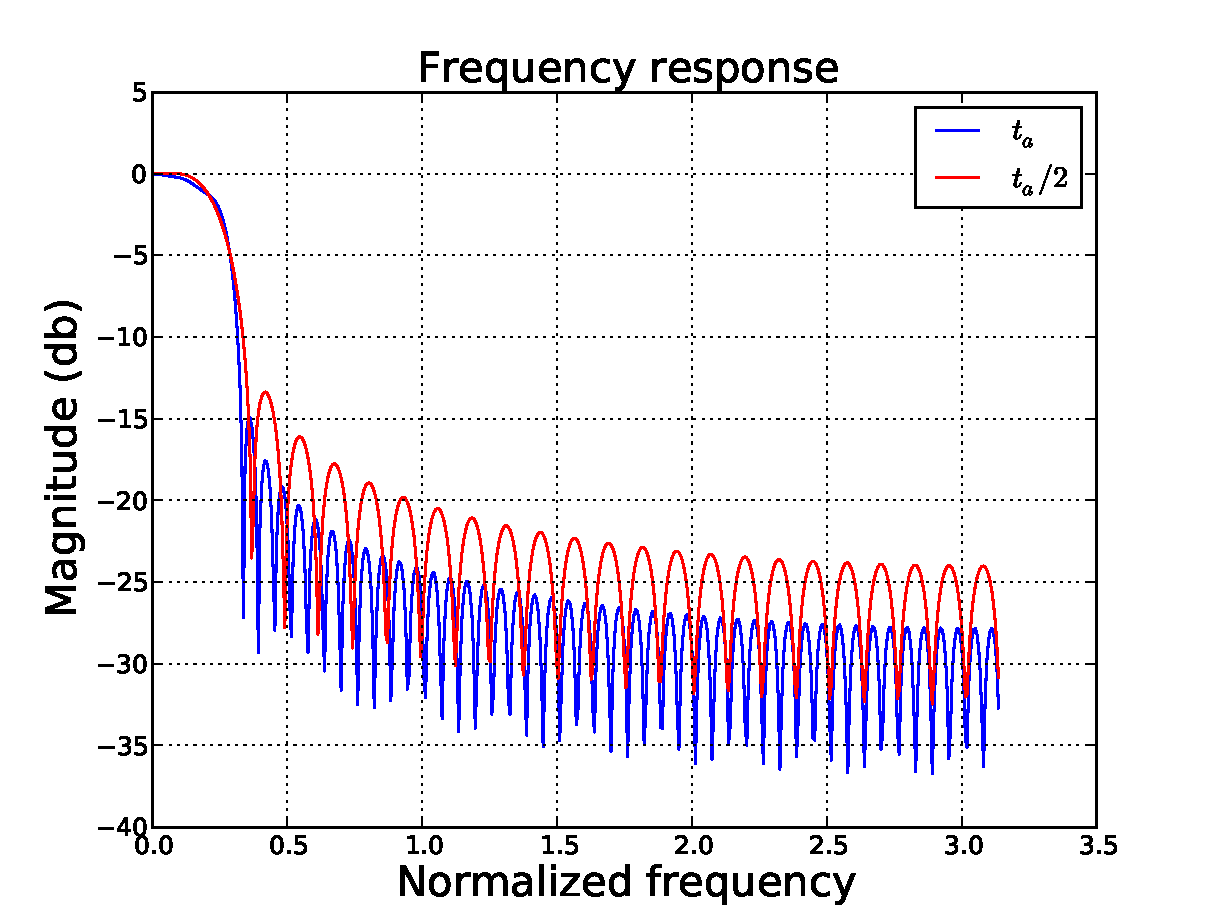
\includegraphics[width=1\textwidth]{./Figures/freq_resp_bessel.pdf}\caption{Frequency 
response of Bessel first kind window}\label{fig:freq_resp_bessel} \end {minipage}
\end{figure*}
\subsection{Theoretical noise estimate and simulation noise}
\label{subsec:noise}
 We show in this section that on shorter baselines, the sinc, the J$_0$ and the BW reduce to the Boxcar window. 
Therefore, we effectively applying a hybrid window in the Fourier plane; a Boxcar on the shorter baselines 
and the WF under consideration on the longer baselines (see Figure \ref{fig:longshortmid-sinc}, \ref{fig:longshortmid-bessel} and 
\ref{fig:longshortmid-butter}). We furthermore evaluated the array
theoretical noise ratio, $R_{\sigma}=\epsilon_{ar,oo}^{bd}/\epsilon_{ar,oo}^{bx}$ predicted in Eq.\ref{eq:noise} of a $2^\circ$ BDWF 
averaging  by the one of boxcar averaging and compared the ratio to the simulation one. For the 
analysis we used a JVLAC measurement set (MS) of 7min30s synthesis with a 1.5s
integration time at 1.4Ghz, with 150 channels of width 125kHz. The MS is filled with 1Jy thermal noise. We then processed boxcar 
averaging and BDWF averaging over 1min30s (width of the time integration) and 12500kHz (channel with). Two overlaps BDWF are presented, 
the first overlap over 2min60s across time and 3125kHz across frequency; the second overlap over 3min45s across time and 6250kHz across 
frequency.
\begin{figure*}
 \centering
  \begin{minipage}{0.38\linewidth}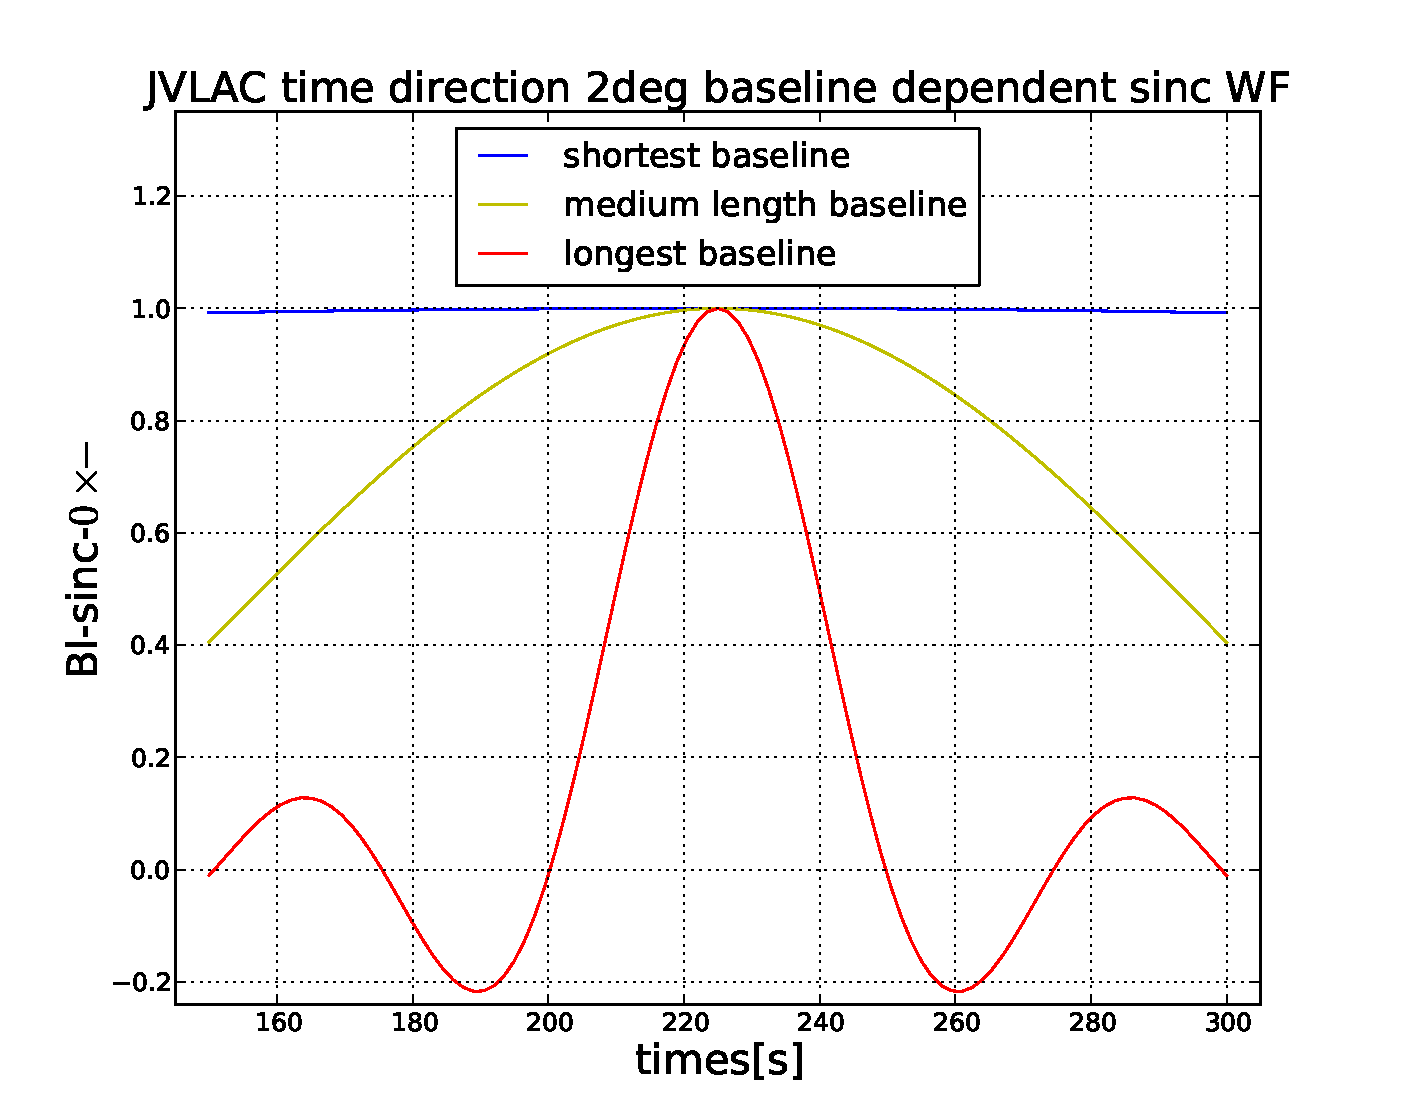
\includegraphics[width=1\textwidth]{./Figures/longshortmid-sinc.pdf}
  \caption{Time direction Bl-sinc-W0 of the shortest, medium and longest baseline}\label{fig:longshortmid-sinc}
  \end{minipage}
  \hspace{1cm}
  \begin{minipage}{0.38\linewidth}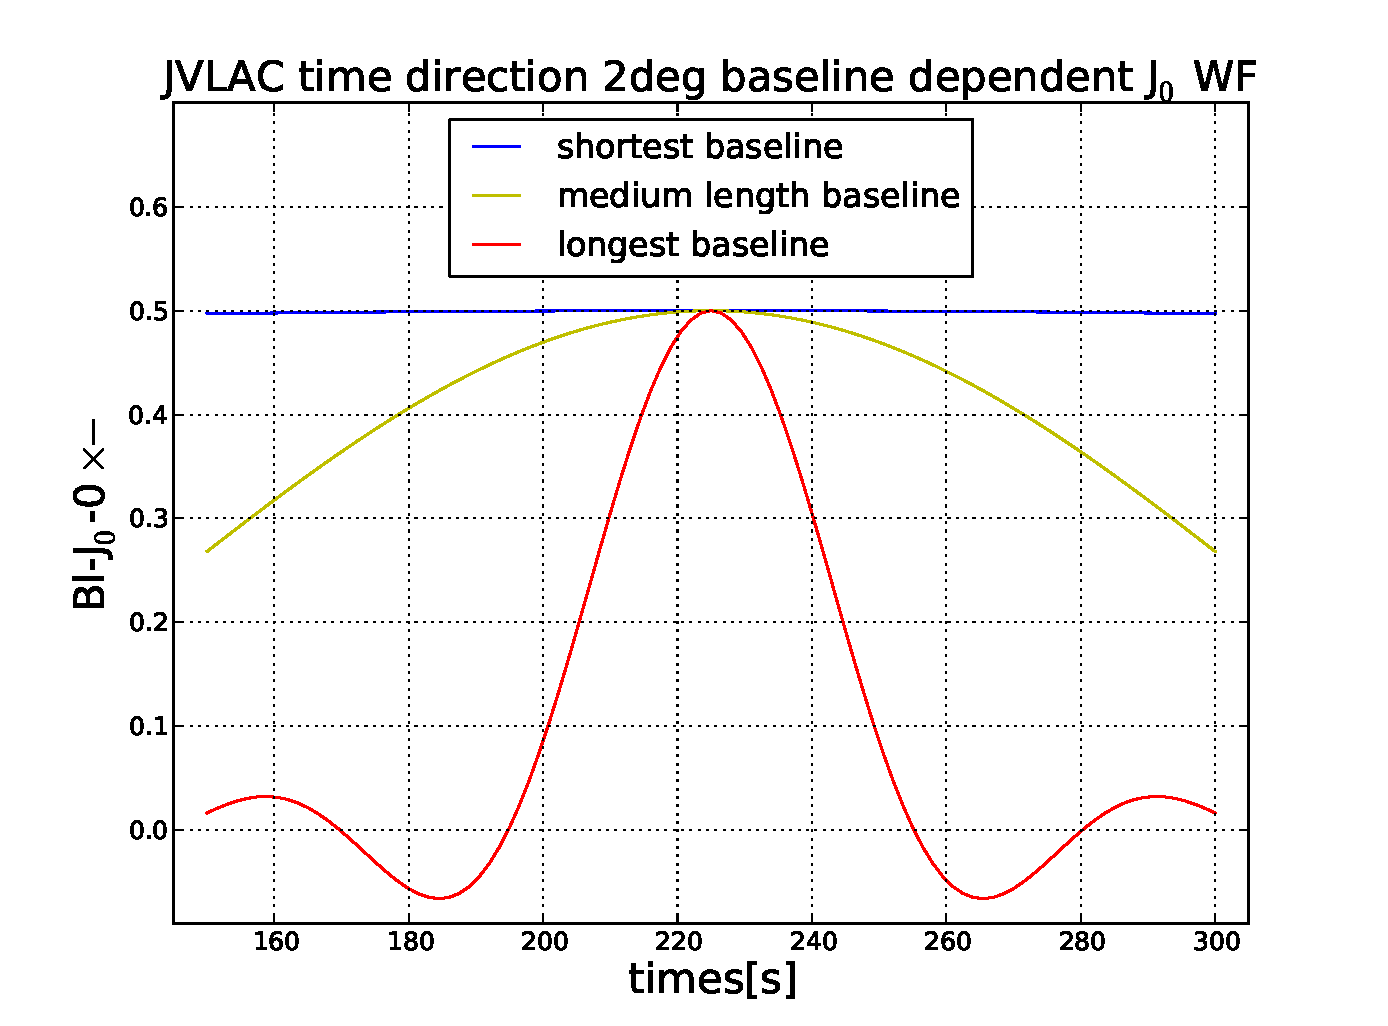
\includegraphics[width=1\textwidth]{./Figures/longshortmid-bessel.pdf}
  \caption{Time direction Bl-J$_0$-W0 of the shortest, medium and longest baseline}\label{fig:longshortmid-bessel}
  \end{minipage}\\
  \begin{minipage}{0.38\linewidth}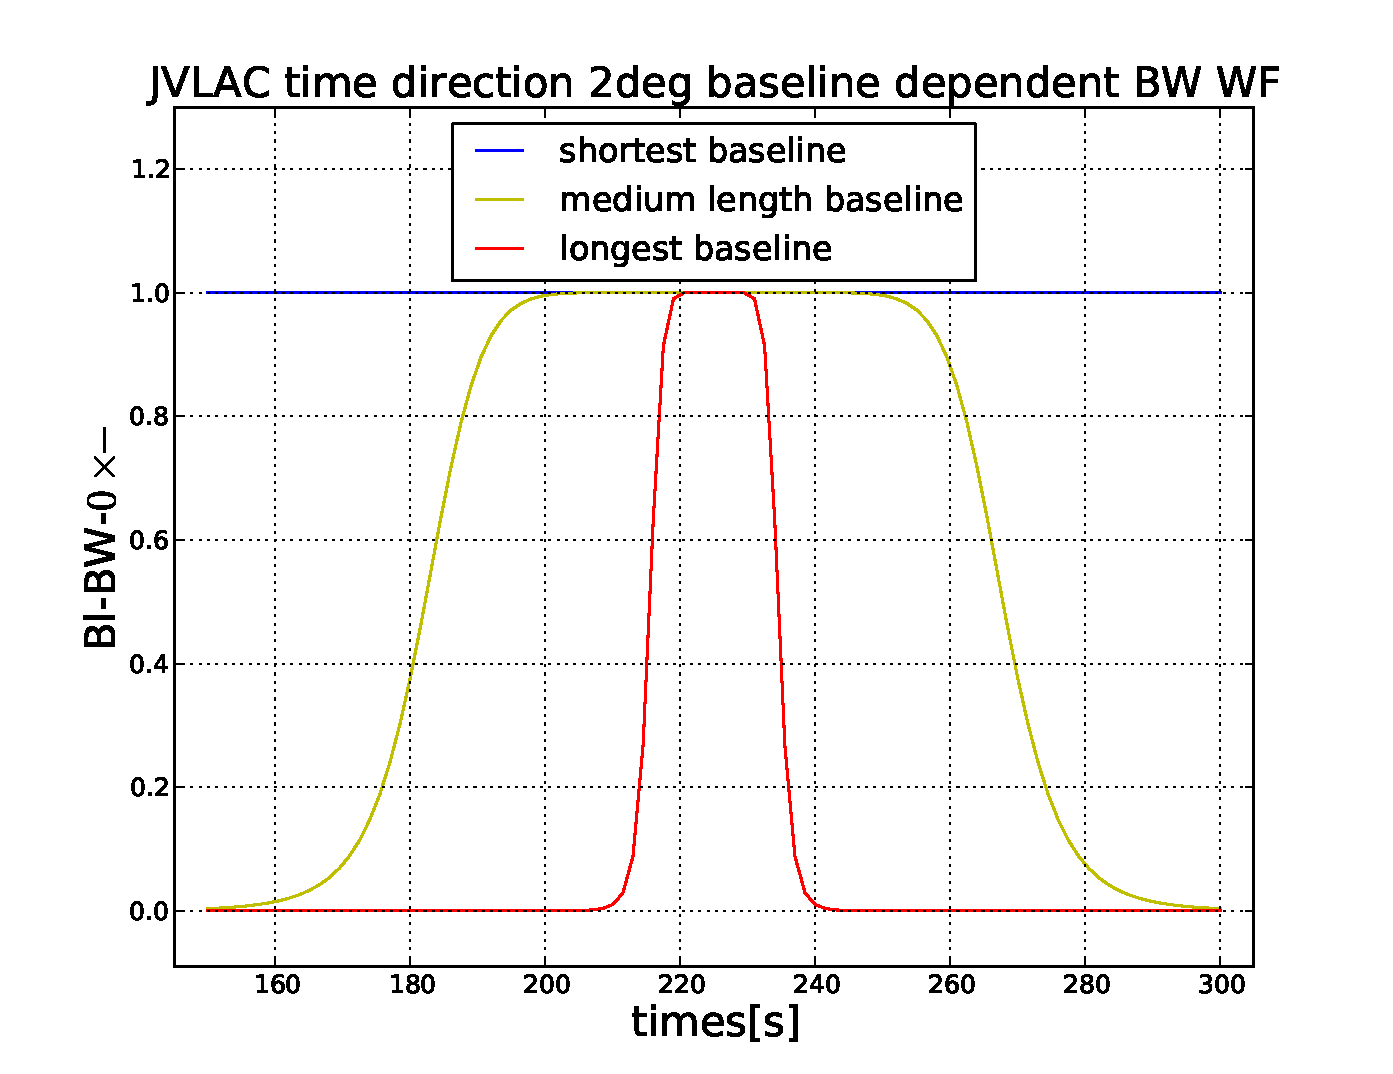
\includegraphics[width=1\textwidth]{./Figures/longshortmid-butter.pdf}\\
  \caption{Time direction Bl-BW-W0 of the shortest, medium and longest baseline}\label{fig:longshortmid-butter}
  \end{minipage}
% \end{figure*}
% \begin{figure*}
%  \centering
    \begin{minipage}{0.38\linewidth}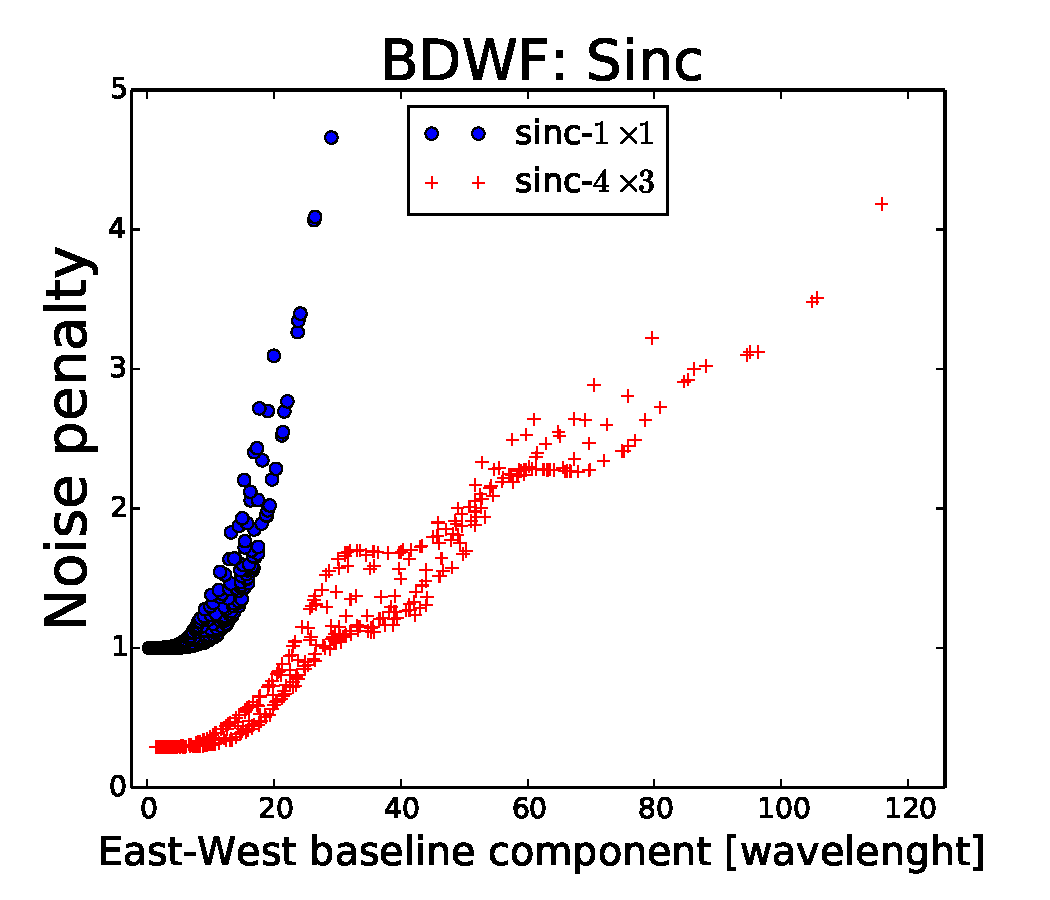
\includegraphics[width=1\textwidth]{./Figures/per-baseline-noise-ratio-sinc.pdf}
  \caption{Per baseline noise ratio of Bl-sinc-W$n_{lt}\times n_{l\nu}$ and averaging}\label{fig:per-baseline-noise-ratio-sinc}
  \end{minipage}
  \hspace{1cm}
  \begin{minipage}{0.38\linewidth}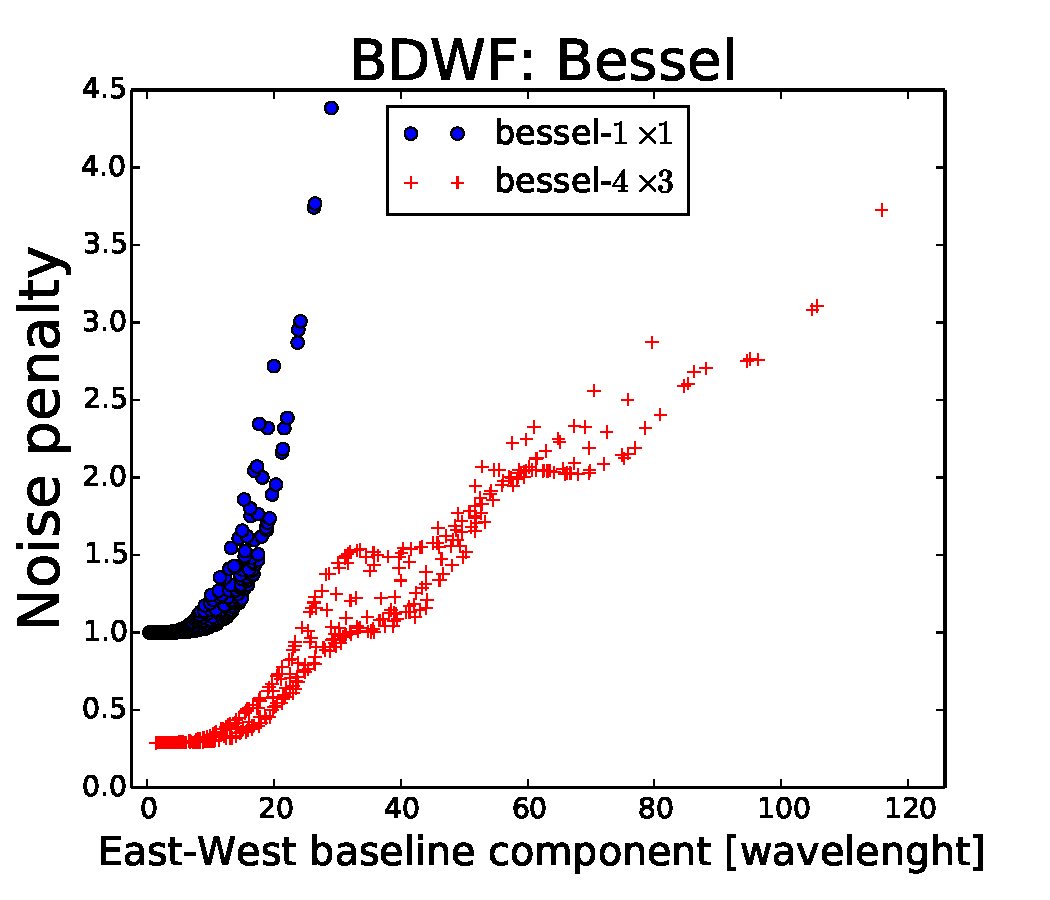
\includegraphics[width=1\textwidth]{./Figures/per-baseline-noise-ratio-bessel.pdf}\\
  \caption{Per baseline noise ratio of Bl-J$_0$-W$n_{lt}\times n_{l\nu}$ and 
averaging}\label{fig:per-baseline-noise-ratio-bessel}\end{minipage}
  \begin{minipage}{0.38\linewidth}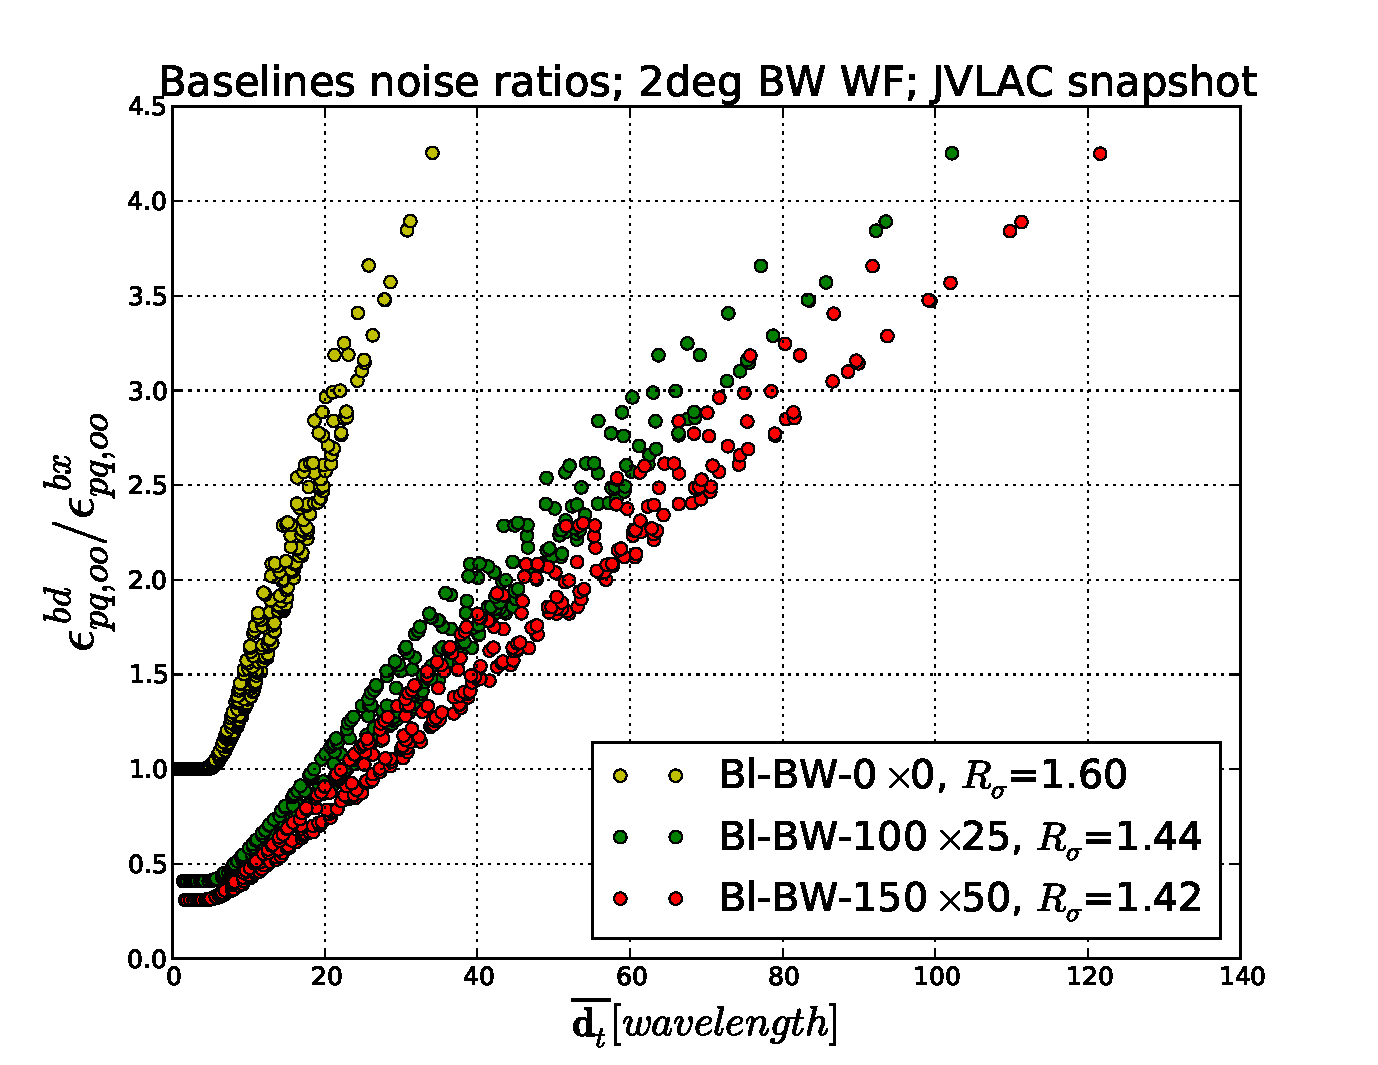
\includegraphics[width=1\textwidth]{./Figures/per-baseline-noise-ratio-BW.pdf}
  \caption{Per baseline noise ratio of Bl-BW-W$n_{lt}\times n_{l\nu}$ and averaging}\label{fig:per-baseline-noise-ratio-BW}
  \end{minipage}
\end{figure*}
\begin{itemize}
 \item In Figure \ref{fig:per-baseline-noise-ratio-sinc}, \ref{fig:per-baseline-noise-ratio-bessel} 
and \ref{fig:per-baseline-noise-ratio-BW} each \textit{dot mark} is the ratio 
\footnote{$\epsilon^{bd}_{pq,oo}/\epsilon^{bx}_{pq,oo}$, see 
Eq.\ref{eqv:linear} for a recall of $\epsilon^{bd}_{pq,oo}$ and $\epsilon^{bx}_{pq,oo}$.} of per baseline centre pixel theoretical rms 
noise ($\epsilon^{bd}_{pq,oo}$) of a $2^\circ$ BDWF 
averaging  by the one of boxcar averaging ($\epsilon^{bx}_{pq,oo}$). The ratio is plotted as a function of 
$\overline{\mathbf{d}}_t$ (the mean of the baseline $(u,v)$ distance). The figures show that, the noise increases with baseline 
length.
   \item On shorter baselines, the noise estimate of BDWF averaging is approximately the same with the one 
of boxcar averaging. Also, on shorter baselines, the noise drops significantly with the number of  overlap time and frequency bins. As 
mention above, this is because on 
shorter  baselines, the BDWF are closer to the boxcar window, and when the number of overlap time  and 
frequency  bins increases, the ratio:
 $\epsilon^{bd}_{pq,oo}/\epsilon^{bx}_{pq,oo} \approx \sqrt{n_t n_{\nu}/\big((n_t + 2n_{ovlpt})(n_{\nu} + 
2n_{ovlp\nu})\big)}$.%\bigg)^{\frac{1}{2}}
\end{itemize}
The table below summarized the array theoretical rms noise ratio and the simulation one. One do not need to worry about a perfect 
agreement of the theoretical noise results with the simulation one. Unfortunately, the theoretical noise results are the rms noise of the 
sky map centre pixel while the simulation results are an average of the sky map overall pixels rms noise.\\
\\
\begin{tabular}{*3{c}}
 \multicolumn{3}{|c|}{}\\
\hspace{0.15cm}\begin{tabular}{l*{6}{c}r}
  \hline
  \textbf{\footnotesize BDWF} &\textbf{\footnotesize Theoretical}&\textbf{\footnotesize Simulation}\\
  \hline\hline
  {\footnotesize Bl-sinc-0$\times$0} &{\footnotesize $1.17$} &{\footnotesize $1.23$}\\
  {\footnotesize Bl-sinc-100$\times$25} &{\footnotesize $1.02$} &{\footnotesize $1.18$}\\
  {\footnotesize Bl-sinc-150$\times$50} &{\footnotesize $1.03$} &{\footnotesize $1.27$}\\
  \hline
  {\footnotesize Bl-J$_0$-0$\times$0} &{\footnotesize  $1.11$}&{\footnotesize  $1.14$}\\
  {\footnotesize Bl-J$_0$-100$\times$25} &{\footnotesize  $0.91$}&{\footnotesize  $1.08$}\\
  {\footnotesize Bl-J$_0$-150$\times$50} &{\footnotesize  $0.92$}&{\footnotesize  $1.13$}\\
  \hline
  {\footnotesize Bl-BW-0$\times$0} & {\footnotesize $1.16$}&{\footnotesize  $1.55$}\\
  {\footnotesize Bl-BW-100$\times$25} & {\footnotesize $1.44$}&{\footnotesize  $1.49$}\\
  {\footnotesize Bl-BW-150$\times$50} & {\footnotesize $1.42$}&{\footnotesize  $1.44$}
\end{tabular}
\end{tabular}
\section{Simulations and results}
In order to test the approaches described in sections \ref{baseline1} and \ref{baseline2}, multiple tests are performed on JVLAC 
simulated MS. This section summarized and discussed those results. Two MS are used in 
the simulation, a high resolution MS (HR-MS) that contains the observed JVLAC data of short integration time and frequency and a low 
resolution 
MS (LR-MS) where the results of boxcar averaging or BDWF averaging are saved. In order to apply an overlap BDWF  the following 
conditions have to be satisfied:
\begin{enumerate}
 \item If $t^{hrms}_{start}$ and $t^{lrms}_{start}$ are the starting time of the HR-MS and LR-MS respectively and  $\Delta t^{hrms}$ the 
HR-MS integration time, then 
      %\begin{eqnarray*}
	    $t^{lrms}_{start}\geq t^{hrms}_{start} + 2n_{ovlpt}\times \Delta t^{hrms}$. 
      %\end{eqnarray*}
  \item If $t^{hrms}_{end}$ and $t^{lrms}_{end}$ are the ending time of the HR-MS and LR-MS respectively, then 
      %\begin{eqnarray*}
	    $t^{lrms}_{end}\leq t^{hrms}_{end} + 2n_{ovlpt}\times \Delta t^{hrms}$. 
      %\end{eqnarray*}
 \item If $\nu^{hrms}_{start}$ and $\nu^{lrms}_{start}$ are the starting frequency of the HR-MS and LR-MS respectively and  $\Delta 
\nu^{hrms}$ the HR-MS channel width, then 
      %\begin{eqnarray*}
	    $\nu^{lrms}_{start} \geq \nu^{hrms}_{start} + 2n_{ovlp\nu}\times \Delta \nu^{hrms}$. 
      %\end{eqnarray*}
 \item If $\nu^{hrms}_{end}$ and $\nu^{lrms}_{end}$ are the ending frequency of the HR-MS and LR-MS respectively, then 
      %\begin{eqnarray*}
	    $\nu^{lrms}_{end} \leq \nu^{hrms}_{end} + n_{ovlp\nu}\times \Delta \nu^{hrms}$. 
      %\end{eqnarray*}
\end{enumerate}
\subsection{Smearing elimination and out FoV suppression}
The study considered $40$ different sky models each  containing a 1Jy source; the sky models differ from each other by the source 
coordinates. 
The reason for having  only one source in the sky model is to avoid standard imaging artefacts in the sky maps which 
can affect the brightness of sources. Another obvious reason is the  CLEAN algorithm \citep{cornwell1999deconvolution}, which does not 
create 
perfect clean maps. Each  sky model is simulated 
with a JVLAC HR-MS of 7min30s synthesis, with a $\Delta t^{hrms}=1.5s$ integration 
time at 1.4GHz,  with 150 channels width $\Delta \nu^{hrms}$=125kHz.  Each HR-MS is then processed with boxcar averaging and BDWF 
averaging the results are saved into a JVLAC LR-MS of one timeslot of with  150s,  with 1 channel of width 6.25MHz. The study also 
considered, $\{t^{hrms}_{start},\nu^{hrms}_{start}\}=\{0s,125kHz\}$, $\{t^{lrms}_{start},\nu^{lrms}_{start}\}=\{150s,6250kHz\}$, 
$\{t^{hrms}_{end},\nu^{hrms}_{end}\}=\{7min30s,18750kHz\}$, $\{t^{lrms}_{end},\nu^{lrms}_{end}\}=\{6min,12500kHz\}$, 
$n_{ovlpt}\in\{0,100,150\}$ 
and $n_{ovlp\nu}\in\{0,25,50\}$. 

The source flux density as a function of the source distance from the phase centre is depicted in Figures \ref{fig:Bl-sinc-FoV2} to 
\ref{fig:Bl-butter-FoV4}.
The study in Figure \ref{fig:Bl-sinc-FoV2}, \ref{fig:Bl-bessel-FoV2} and \ref{fig:Bl-butter-FoV2} 
compared boxcar averaging with $2^{\circ}$ FoV of Bl-sinc-$n_{ovlpt}\times n_{ovlp\nu}$, Bl-J$_0$-$n_{ovlpt}\times n_{ovlp\nu}$ and  
Bl-BW-$n_{ovlpt}\times n_{ovlp\nu}$ respectively. A study with a $2^{\circ}$ FoV suggest that: "\textit{Regime 1}" is defined from 
$0^\circ$ to $1^\circ$; "\textit{Regime 2}" from $1^\circ$ to $1.5^\circ$ and "\textit{Regime 3}" from $1.5^\circ$ to infinity.
The study in Figure \ref{fig:Bl-sinc-FoV4}, \ref{fig:Bl-bessel-FoV4} and \ref{fig:Bl-butter-FoV4} 
compared boxcar averaging with $4^{\circ}$ FoV of Bl-sinc-$n_{ovlpt}\times n_{ovlp\nu}$, Bl-J$_0$-$n_{ovlpt}\times n_{ovlp\nu}$ and  
Bl-BW-$n_{ovlpt}\times n_{ovlp\nu}$ respectively.  A study with a $4^{\circ}$ FoV suggest that: "\textit{Regime 1}" is defined from 
$0^\circ$ 
to $2^\circ$; "\textit{Regime 2}" from $2^\circ$ to $3^\circ$ and "\textit{Regime 3}" from $3^\circ$ to infinity. 
% 
% We considered three cases of the 
% sinc ($Bl$-$sinc$-$W n_{t,ovlp} \times n_{\nu,ovlp}$), the Bessel 
% of the first kind of order zero ($Bl$-J$_0$-$W n_{t,ovlp} \times n_{\nu,ovlp}$) and the Butterwordth ($Bl$-$BW$-$W n_{t,ovlp} \times 
% n_{\nu,ovlp}$),  with  $n_{t,ovlp}\in\{0,100,150\}$ and $n_{\nu,ovlp}\in\{0,25,50\}$). We evaluated the loss in signal 
% amplitude with longer LR-MS integration time intervals $\Delta t^{lrms}=150s$ and wider LR-MS integration frequency intervals $\Delta 
% \nu^{lrms}=6250kHz$. We furthermore evaluated the  noise ratio, $\mathcal{R}_{\sigma}=\frac{\sigma_{w}}{\sigma_{Avg}}$ (with $\sigma_{w}$  
% the resulting noise of the filter under consideration and $\sigma_{Avg}$ the noise of simple averaging).\\
% % $r$: source position in degrees.}
The results show that:
\begin{itemize}
 \item "\textit{Regime 1}" (FoV recovery): The source flux density is recovered with the BDWF averaging compared to the boxcar averaging. 
Also, as the overlap time and frequency bins increase, the source flux density becomes optimal with the overlap sinc and J$_0$ (see the 
green and the red curve from Figures \ref{fig:Bl-sinc-FoV2} to \ref{fig:Bl-bessel-FoV4}) which is not the case with the overlap BW as shown 
in Figures \ref{fig:Bl-butter-FoV2} and \ref{fig:Bl-butter-FoV4} (the green and the red curve).
\item "\textit{Regime 2}" (nearby sources suppression): The source flux density is suppressed using boxcar averaging compared to 
BDWF averaging without overlap bins (see Bl-sinc-$0\times0$, Bl-J$_0$-$0\times0$ and Bl-BW-$0\times0$ shown  from Figure 
\ref{fig:Bl-sinc-FoV2} to \ref{fig:Bl-butter-FoV4}). It is also seen from Figure \ref{fig:Bl-sinc-FoV2} to \ref{fig:Bl-bessel-FoV4} 
(the green and the red curve) that, the source flux density is suppressed within $\approx 25\%$ of the regime using boxcar 
averaging than the sinc and J$_0$ overlap BDWF averaging while within $\approx 75\%$ of the regime the sinc and J$_0$ overlap BDWF 
averaging suppressed the source compared to the boxcar averaging. The performance of the overlap BW BDWF averaging is not accurate in this 
regime.
\item "\textit{Regime 3}" (far away sources attenuation): It appears on Figures \ref{fig:Bl-sinc-FoV2} to \ref{fig:Bl-bessel-FoV4}  that  
the curves of boxcar averaging (see Bx-avg-$0\times0$) mid that of Bl-sinc-$0\times0$ and Bl-J$_0$-$0\times0$ which implied an equivalent 
flux density 
attenuation while the curve of 
Bl-sinc-$100\times25$, Bl-sinc-$150\times50$, Bl-J$_0$-$100\times25$ and Bl-J$_0$-$150\times50$ are below the one of Bx-avg-$0\times0$ which 
implied 
that the overlap sinc and J$_0$ BDWF attenuated the source in the regime more than boxcar averaging. Also, as the overlap time and frequency 
bins increase, the attenuation becomes significant. The similar results occurs $1^{\circ}$ away from the regime 
starting interval with BW BDWF averaging.
\end{itemize}
% 
% suppression
% the overlaps filters are below the one of boxcar averaging when the source is out
% 
% (Far away sources suppression): Also note that for the overlap filters, out FoV source suppression is 
% significantly improved.  When
% looking at these figures, it appears that the curves of the overlaps filters are below the one of boxcar averaging when the source is out 
% FoV ("\textit{regime 3}"). 
%    When
% looking at these figures, it appears that the baseline dependent sinc conserved the signal in \textit{regime 1} compared to the 
% baseline dependent J$_0$, while the baseline dependent J$_0$ suppressed the 
% signal in \textit{regime 3} compared to the baseline dependent sinc. However, the reason for 
% this is that
% the MLW of the sinc is narrower than that of J$_0$ and the SLR of J$_0$ drops faster compared to the SLR of the sinc.
% 
% When performing the baseline dependent filters, smearing was eliminated within the FoV while we compressed 
% the data by integrating over a large time interval and wider frequency interval of a LR-MS. However,
% the overlap baseline dependent filters significantly suppressed the source  when the source is out of the FoV  to a greater extent than 
% boxcar averaging. Thus,
% in all cases the SNR obtained using these methods is greater than obtained using boxcar averaging even as there is loss in 
% sensitivity.
\subsection{Maximum integration}
In this section, the maximum frequency and time integration intervals  that can be 
considered in the frequency and the time 
directions without loss of signal amplitude is evaluated. The study considered $6$ sky 
models each  containing 1Jy source; the sky models differ by the source 
coordinates with radius $r\in\{0.09^\circ,0.25^\circ,0.5^\circ,1^\circ,1.5^\circ, 2^\circ\}$. The study compared the results of  boxcar 
averaging to a $2^\circ$ BDWF averaging. As mention above, a $2^{\circ}$ FoV suggest that: "\textit{Regime 1}" 
is defined from $0^\circ$ to $1^\circ$; "\textit{Regime 2}" from $1^\circ$ to $1.5^\circ$ and "\textit{Regime 3}" from $1.5^\circ$ to 
infinity. Therefore, a sky model with a source radius $r\in\{0.09^\circ,0.25^\circ,0.5^\circ,1^\circ\}$ belongs to "\textit{Regime 1}", 
$r= 1.5^\circ$ belongs to  "\textit{Regime 2}" and $r=2^\circ$ to "\textit{Regime 3}".
\subsubsection{Frequency direction}
Boxcar and BDWF averaging are processed across the frequency direction.
Each of the sky models is simulated with a JVLAC HR-MS of 1 timeslot of width $\Delta t^{hrms}=0.1s$ at $1.4$GHz. The raison of a short 
HR-MS 
integration time is to avoid time direction smearing. The simulation considered 150 channels and varied the channels width $\Delta 
\nu^{hrms}$ in the range $[125,1187.5]$kHz. The result of the process was saved into a LR-MS of 1 timeslot of width $\Delta 
t^{lrms}=0.1s$ at $1.4$GHz with 1 
channel of width $\Delta \nu^{hrms}\times50$kHz. We considered $\nu^{hrms}_{start}=\Delta \nu^{hrms}kHz$, 
$\nu^{lrms}_{start}=\nu^{hrms}_{start}\times50 kHz$, $\nu^{hrms}_{end}=\nu^{hrms}_{start}\times150 kHz$ and 
$\nu^{lrms}_{end}=\nu^{hrms}_{start}\times100 kHz$.

The source flux density as a function of the channel width is depicted in Figures \ref{fig:max-integ-freq-sinc-w1x1-fov2} to 
\ref{fig:max-integ-freq-butter-w1x50-fov2}. The study compared the maximal channel width of the boxcar frequency  averaging 
(Bx-avg-$-\times 0$) 
with that of  $2^{\circ}$ FoV BDWF frequency averaging (Bl-sinc-$-\times 0$, Bl-sinc-$-\times 50$, Bl-J$_0$-$-\times 0$, Bl-J$_0$-$-\times 
50$, Bl-BW-$-\times 0$ and Bl-BW-$-\times 50$). 
The results show that:
\begin{itemize}
 \item "\textit{Regime 1}":  The BDWF frequency averaging maintained the flux density of the source for wider frequency channels. However, 
it is seen on the Figures that the curve of sources in the regime are closer to the affine line y=1 when the channel width increases.
 \item  "\textit{Regime 2}" and "\textit{Regime 3}": It appears on the Figures that Boxcar frequency averaging attenuated the sources in 
these regime compare to BDWF frequency averaging without overlap while overlap sinc and J$_0$ frequency averaging attenuated the source for 
channels widths between $[6.2,12.6]$ compare to the boxcar. 
\end{itemize}
\subsubsection{Time direction}
Boxcar and BDWF averaging are processed across the time direction.
 Each of the sky models is simulated with a JVLAC HR-MS of $300$ timeslots of width $\Delta t^{hrms}s$ at 1.4GHz. The value of  
$\Delta t^{hrms}$ is chosen within the range $[0.5,5.5]$. The simulation considered  1 channel of width $\Delta \nu^{hrms}=125kHz$ and the 
results of the process was saved into a LR-MS of $100\times\Delta t^{hrms}s$ synthesis, with a $100\times\Delta t^{hrms}s$ 
integration time at 1.4GHz, with 
1 channel of width $125kHz$. We considered $t^{hrms}_{start}=0s$, $t^{lrms}_{start}=100\times\Delta t^{hrms} s$, 
$t^{hrms}_{end}=300\times\Delta t^{hrms}s$ and $t^{lrms}_{end}=200\times\Delta t^{hrms}s$.

The source flux density as a function of the integration time width is depicted in Figures \ref{fig:max-integ-time-sinc-w1x1-fov2} to 
 \ref{fig:max-integ-time-butter-w100x1-fov2}. The study compared the maximal integration time width of the boxcar time  averaging 
(Bx-avg-$0\times -$) 
with that of  $2^{\circ}$ FoV BDWF time averaging (Bl-sinc-$100\times -$, Bl-sinc-$100\times -$, Bl-J$_0$-$0\times -$, 
Bl-J$_0$-$100\times-$, Bl-BW-$0\times -$ and Bl-BW-$100\times -$). 
The results show that:
\begin{itemize}
 \item "\textit{Regime 1}":  The BDWF time averaging maintained the flux density of the source for large integration time. 
However, 
it is seen on the Figures that the curve of sources in the regime are closer to the affine line y=1 when the integration time increases.
 \item  "\textit{Regime 2}" and "\textit{Regime 3}": It appears on the Figures that Boxcar time averaging attenuated the sources in 
these regime compare to BDWF time averaging without overlap while overlap sinc and J$_0$ time averaging attenuated the source in a variable 
integration time range compare to the boxcar (see black and red curve in Figure \ref{fig:max-integ-time-sinc-w100x1-fov2} and 
\ref{fig:max-integ-time-bessel-w100x1-fov2}). The integration time range where the source is attenuated  depends on the 
WF (sinc or J$_0$) and the overlap time bins which cause its to variate. 
\end{itemize}
\subsubsection{Time and frequency direction}
Boxcar and BDWF averaging are processed across the time and the frequency direction.
Each sky model is simulated with a JVLAC HR-MS of $300$ timeslots and  the integration time $\Delta 
t^{hrms}$ is chosen within the range $[0.5,5.5]s$ at $1.4GHz$. The simulation considered $150$ channels of width $\Delta 
\nu^{hrms}$  chosen within the range $[125.,750.]kHz$.  The result of the process was saved into a LR-MS of  $100\times\Delta t^{hrms}s$ 
synthesis, with 
$100\times\Delta t^{hrms}$ integration time and 1 channel of width $50\times\Delta \nu^{hrms}kHz$.  We considered, 
$t^{hrms}_{start}=0s$, $t^{lrms}_{start}=100\times\Delta t^{hrms} s$, $t^{hrms}_{end}=300\times\Delta t^{hrms}s$ and 
$t^{lrms}_{end}=200\times\Delta t^{hrms}s$, $\nu^{hrms}_{start}=\Delta 
\nu^{hrms}kHz$, $\nu^{lrms}_{start}=\nu^{hrms}_{start}\times50 kHz$, $\nu^{hrms}_{end}=\nu^{hrms}_{start}\times150 kHz$ and 
$\nu^{lrms}_{end}=\nu^{hrms}_{start}\times100 kHz$.

The source flux density as a function of the integration time and channels width is depicted in Figures 
\ref{fig:max-integ-timefreq-sinc-w1x1-fov2} to 
 \ref{fig:max-integ-timefreq-butter-w100x50-fov2}. The study compared the maximal integration time and channels width of two dimensional 
boxcar  averaging (Bx-avg-$0\times 0$) 
with that of  $2^{\circ}$ FoV of two BDWF averaging (Bl-sinc-$100\times 50$, Bl-sinc-$100\times 50$, Bl-J$_0$-$0\times 50$, 
Bl-J$_0$-$100\times 50$, Bl-BW-$0\times 50$ and Bl-BW-$100\times 50$). 
The results show that:
\begin{itemize}
 \item "\textit{Regime 1}": BDWF averaging maintained the flux density of the source for large integration time and wide channels widths. 
However, 
it is seen on the Figures that the curve of sources in the regime are closer to the affine line y=1 when the integration time and 
channels width increases.
 \item  "\textit{Regime 2}" and "\textit{Regime 3}":  It appear that the curves of the overlaps sinc and J$_0$ are below the one of boxcar 
averaging for all integrations and channels widths. The 
results suggest that one do not need to worry about sidelobes confusion for large integration time and wide channels widths. 
\end{itemize}

\hspace{-0.64cm}\textbf{Discussion:}
The study describes the performances of the WF under consideration. As presented, the sinc performed well in \textit{Regime 1} compared 
to the J$_0$ while the J$_0$ performed well in \textit{Regime 2} and \textit{Regime 3} compared to the sinc. The great potential  of the 
two dimensional overlap sinc and the J$_0$ is the accurate performance in the three regimes. An interesting improvement of this study is 
the possibility of using WF capable of providing higher dynamic range images. This advanced techniques 
is required by the radio telescopes of the future.
\section{Realistic field synthesis: 3C147}
 \begin{figure*}
    \centering
  \begin{minipage}{0.38\linewidth}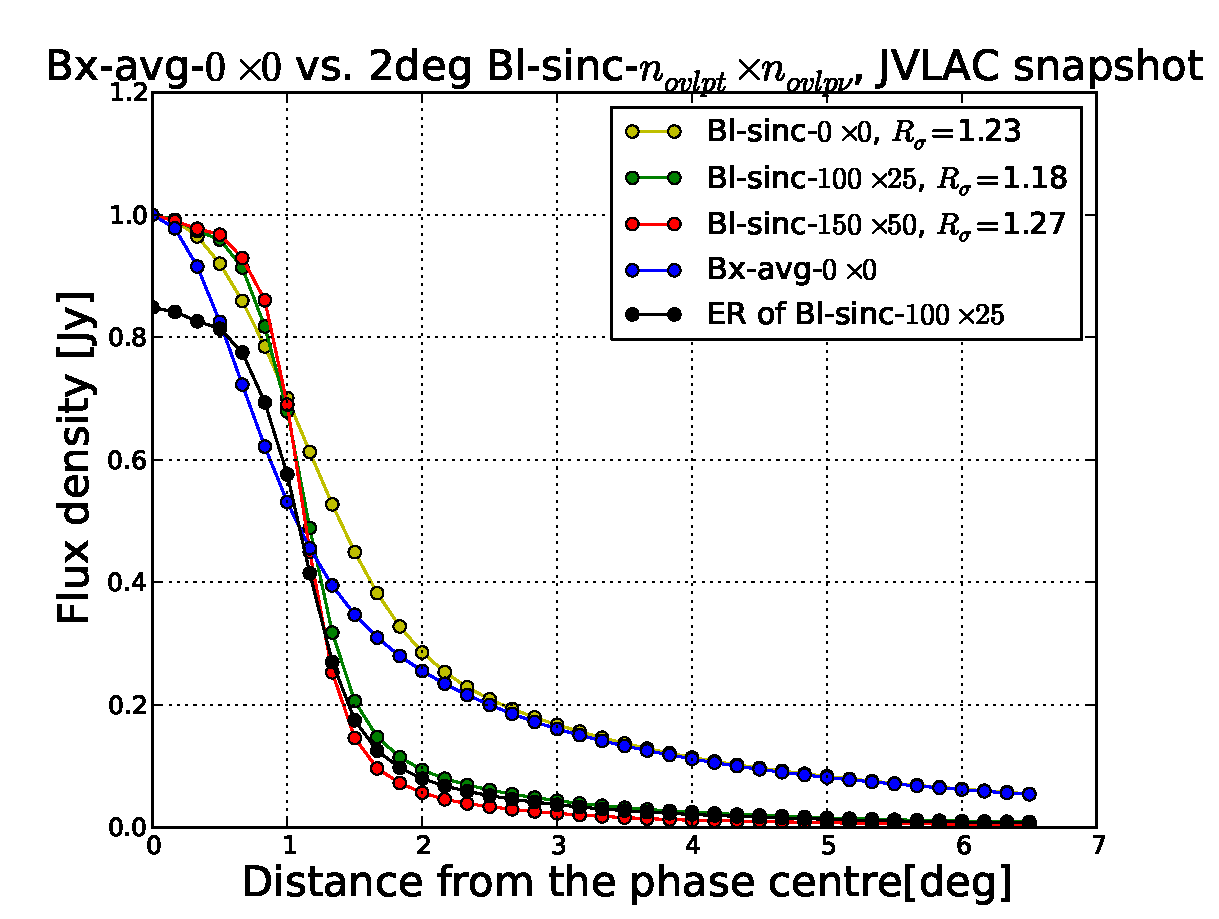
\includegraphics[width=1\textwidth]{./Figures/Bl-sinc-FoV2-vla.pdf}\caption{Time and frequency 
  direction sinc filter applied on a $2^{\circ}$ FoV JVLA surveys observing a 1Jy source move from the phase centre for 150s integration 
  synthesis at 6.25MHz bandwidth, natural weighting.}\label{fig:Bl-sinc-FoV2}\end{minipage}
  \hspace{1cm}
  \begin{minipage}{0.38\linewidth}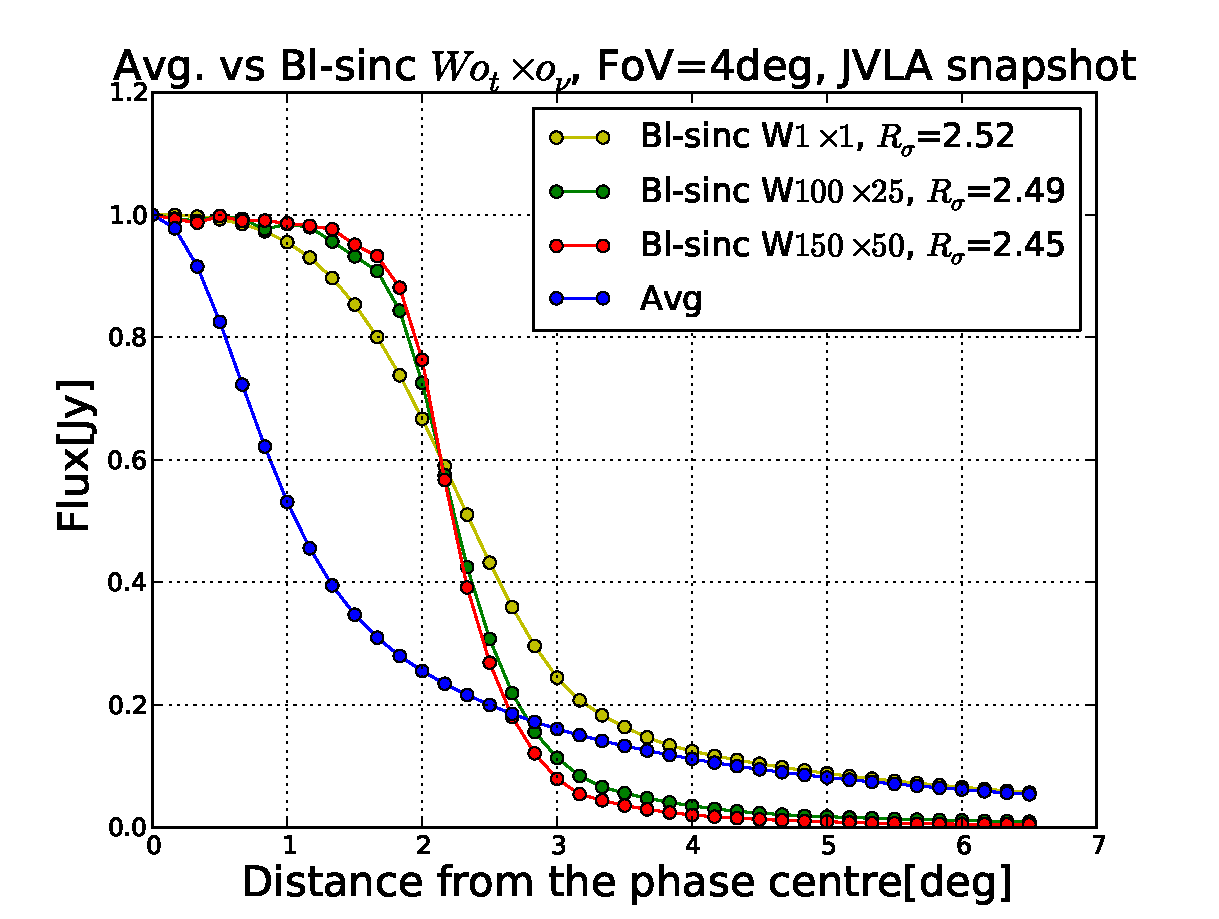
\includegraphics[width=1\textwidth]{./Figures/Bl-sinc-FoV4-vla.pdf}\caption{Time and frequency 
  direction sinc filter applied on a $4^{\circ}$ FoV JVLA surveys observing a 1Jy source move from the phase centre for 150s integration 
  synthesis at 6.25MHz bandwidth, natural weighting.}\label{fig:Bl-sinc-FoV4} 
  \end{minipage}\\
  \begin{minipage}{0.38\linewidth}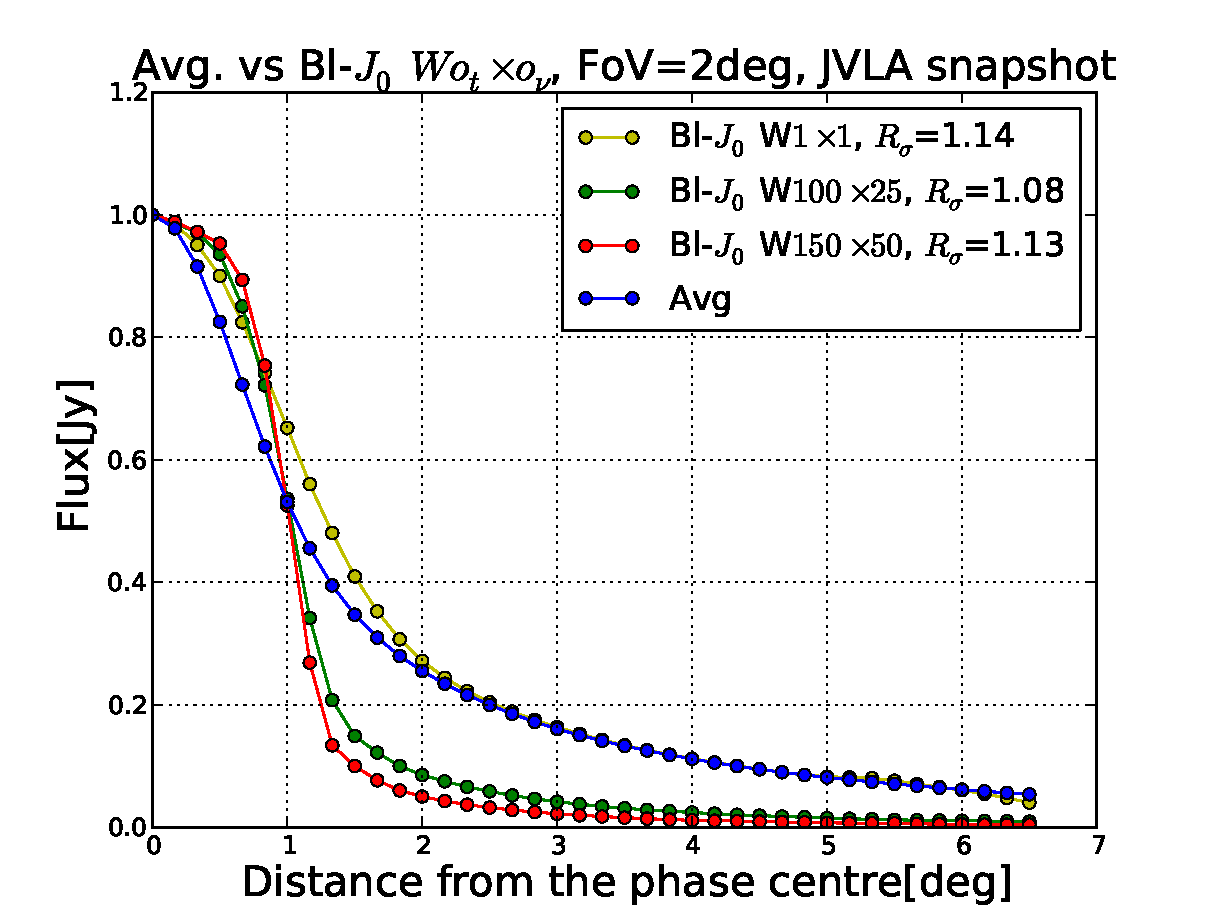
\includegraphics[width=1\textwidth]{./Figures/Bl-bessel-FoV2-vla.pdf}\caption{Time and frequency 
  direction Bessel first kind filter applied on a $2^{\circ}$ FoV JVLA surveys observing a 1Jy source move from the phase centre for 150s 
  integration synthesis at 6.25MHz bandwidth, natural weighting.}\label{fig:Bl-bessel-FoV2}\end{minipage}
  \hspace{1cm}
  \begin{minipage}{0.38\linewidth}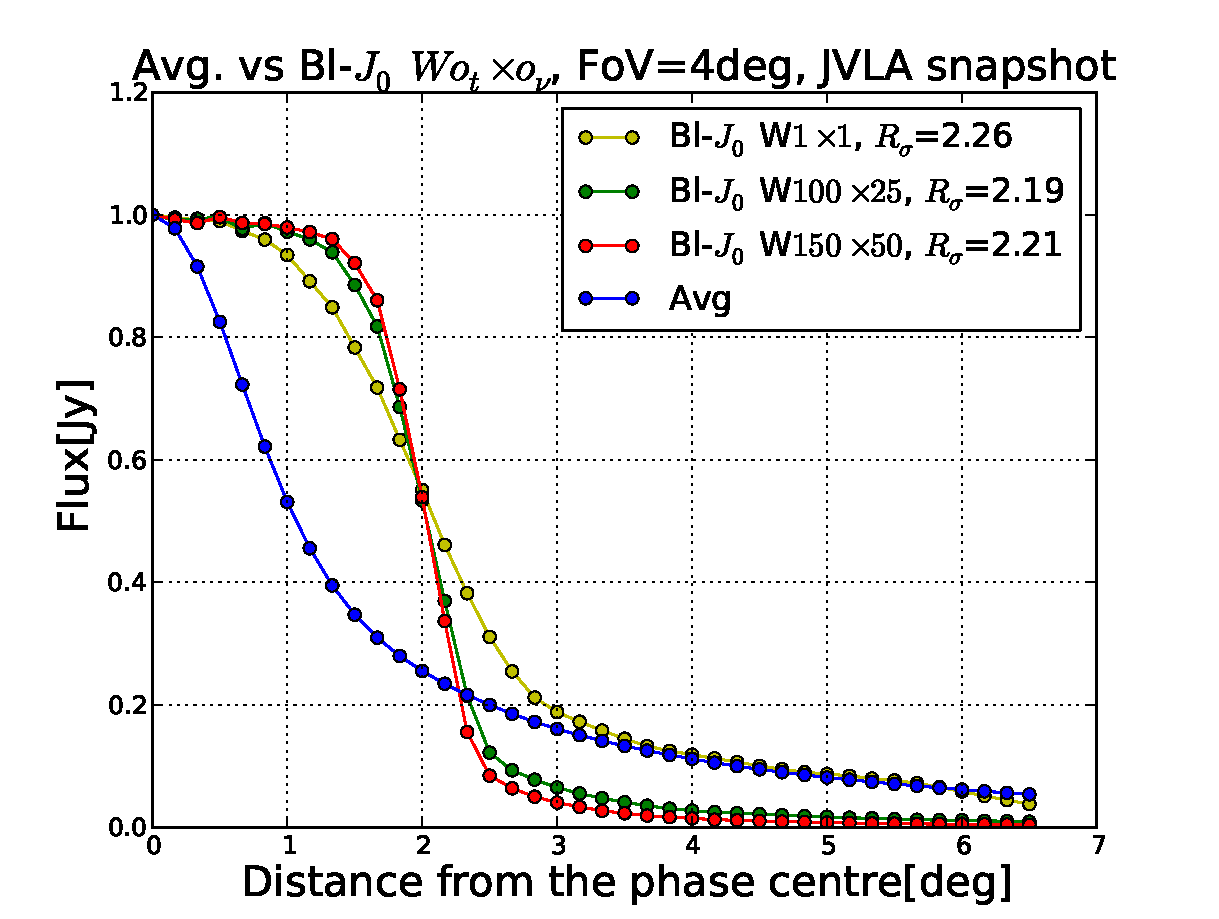
\includegraphics[width=1\textwidth]{./Figures/Bl-bessel-FoV4-vla.pdf}\caption{Time and frequency 
  direction Bessel first kind filter applied on a $4^{\circ}$ FoV JVLA surveys observing a 1Jy source move from the phase centre for 150s 
  integration synthesis at 6.25MHz bandwidth, natural weighting.}\label{fig:Bl-bessel-FoV4}\end{minipage}\\
  \begin{minipage}{0.38\linewidth}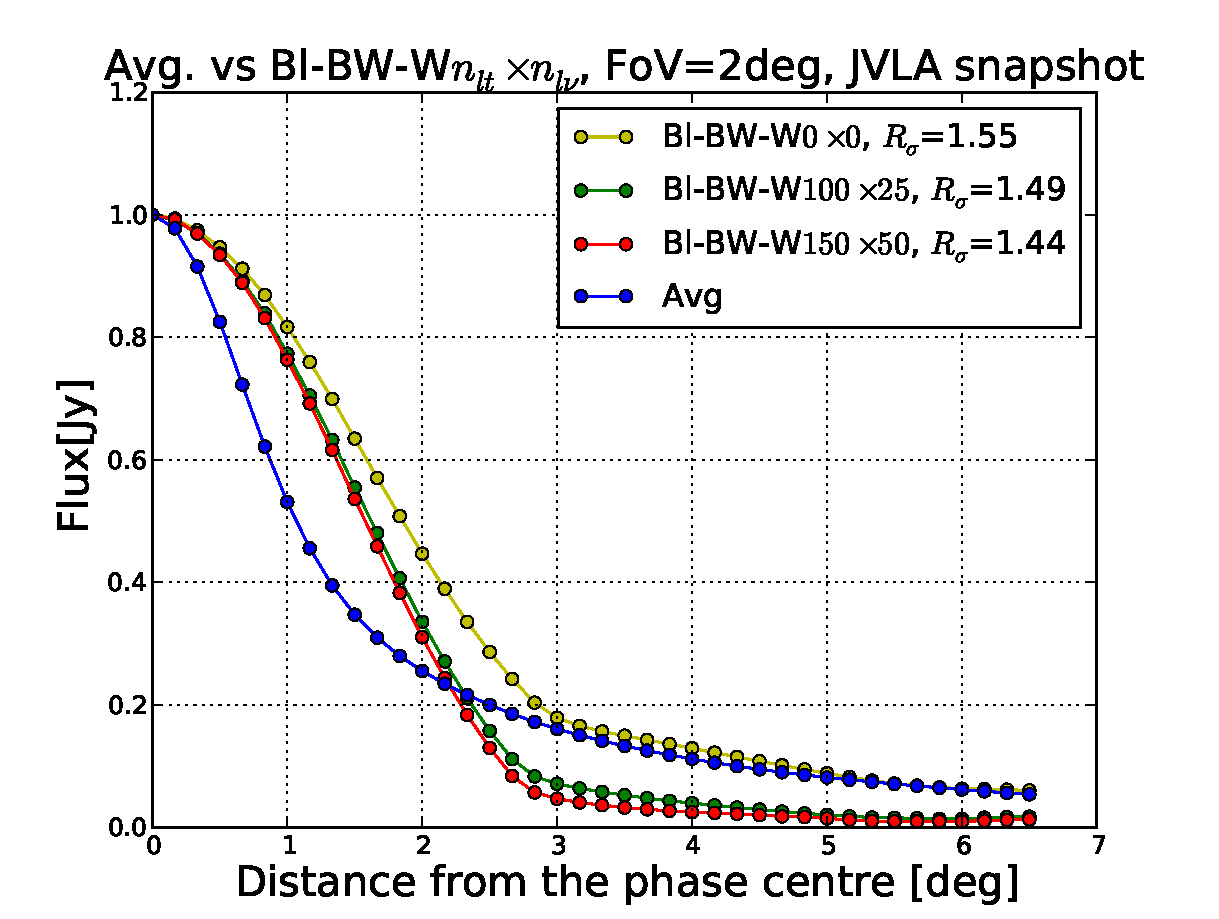
\includegraphics[width=1\textwidth]{./Figures/Bl-butter-FoV2-vla.pdf}\caption{Time and frequency 
  direction Butterwordth filter applied on a $2^{\circ}$ FoV JVLA surveys observing a 1Jy source move from the phase centre for 
  150s integration synthesis at 6.25MHz bandwidth, natural weighting.}\label{fig:Bl-butter-FoV2}\end{minipage}
  \hspace{1cm}
  \begin{minipage}{0.38\linewidth}
  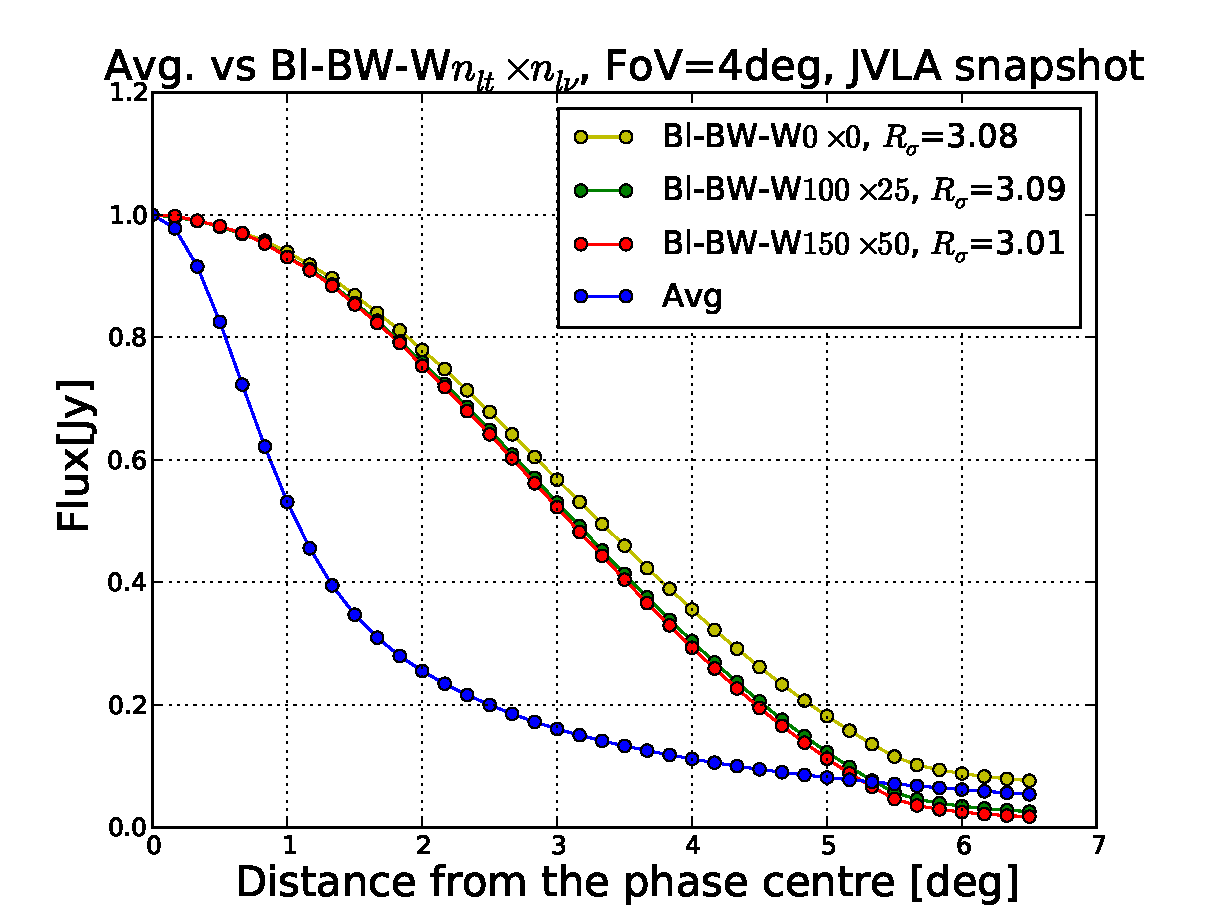
\includegraphics[width=1\textwidth]{./Figures/Bl-butter-FoV4-vla.pdf}
   \caption{Time and frequency 
   direction Butterwordth filter applied on a $4^{\circ}$ FoV JVLA surveys observing a 1Jy source move from the phase centre for 150s 
  integration synthesis at 6.25MHz bandwidth, natural weighting.}
  \label{fig:Bl-butter-FoV4}\end{minipage}
  \caption{Time and frequency 
  direction Butterwordth filter applied on a $4^{\circ}$ FoV JVLA surveys observing a 1Jy source move from the phase centre for 150s 
  integration synthesis at 6.25MHz bandwidth, natural weighting.}
  \end{figure*} 
  \begin{figure*}
    \centering
  \begin{minipage}{0.38\linewidth}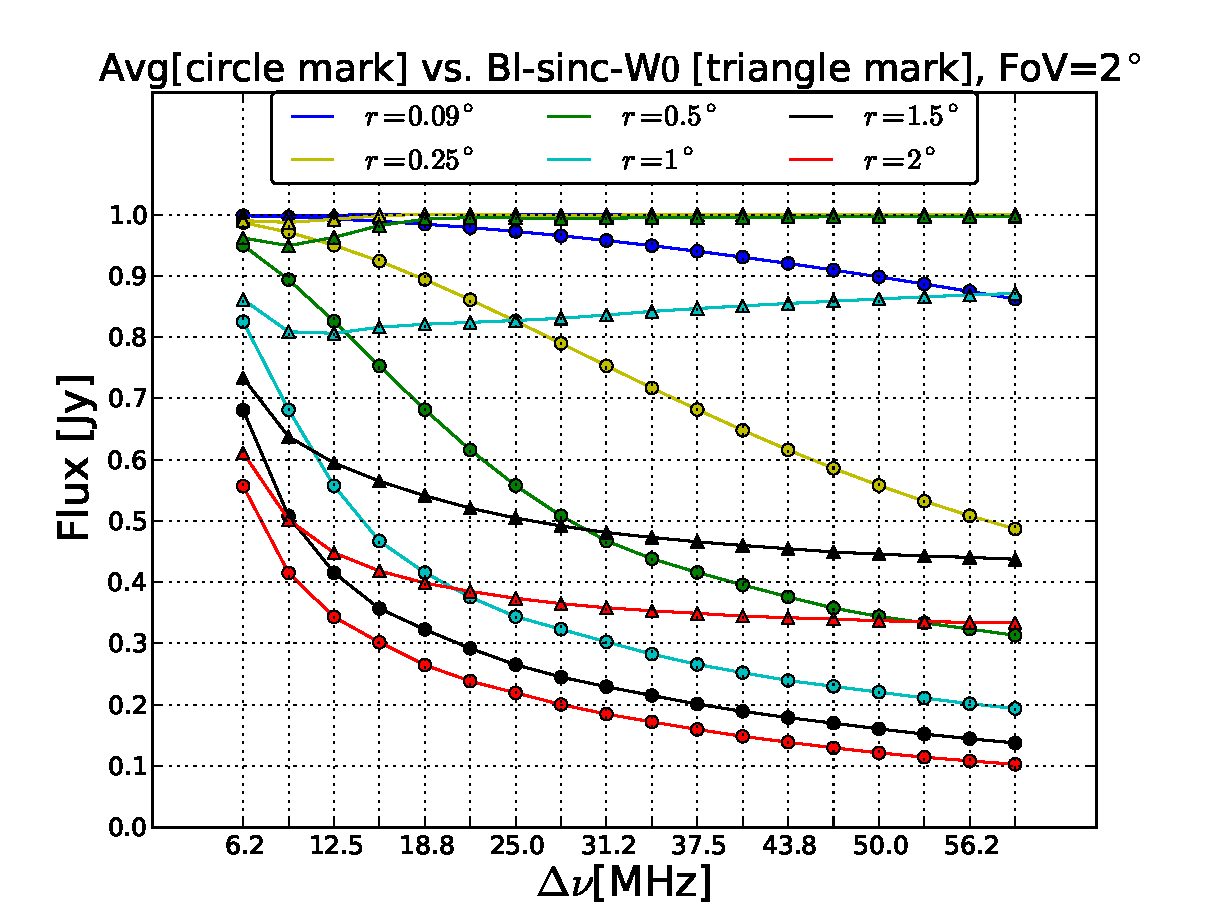
\includegraphics[width=1\textwidth]{./Figures/max-integ-freq-sinc-w1x1-fov2.pdf}
    \caption{Response to a 1Jy source at different positions, as a function of  bandwidth with $2^{\circ}$ frequency sinc filter.}
    \label{fig:max-integ-freq-sinc-w1x1-fov2}
  \end{minipage}
  \hspace{1cm}
  \begin{minipage}{0.38\linewidth}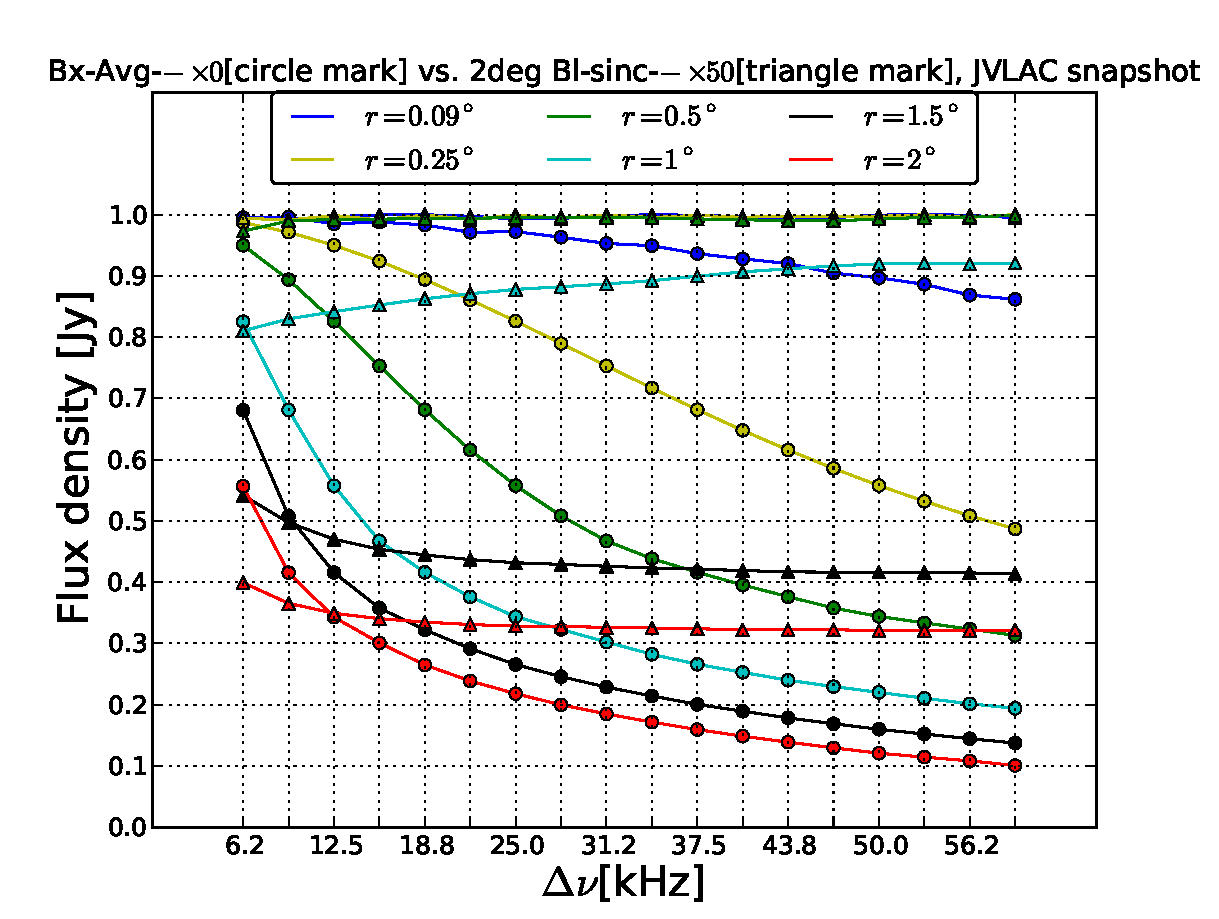
\includegraphics[width=1\textwidth]{./Figures/max-integ-freq-sinc-w1x50-fov2.pdf}
        \caption{Response to a 1Jy source at different positions, as a function of bandwidth with $2^{\circ}$ frequency overlap sinc 
filter.}
        \label{fig:max-integ-freq-sinc-w1x50-fov2}
        \end{minipage}\\
  \begin{minipage}{0.38\linewidth}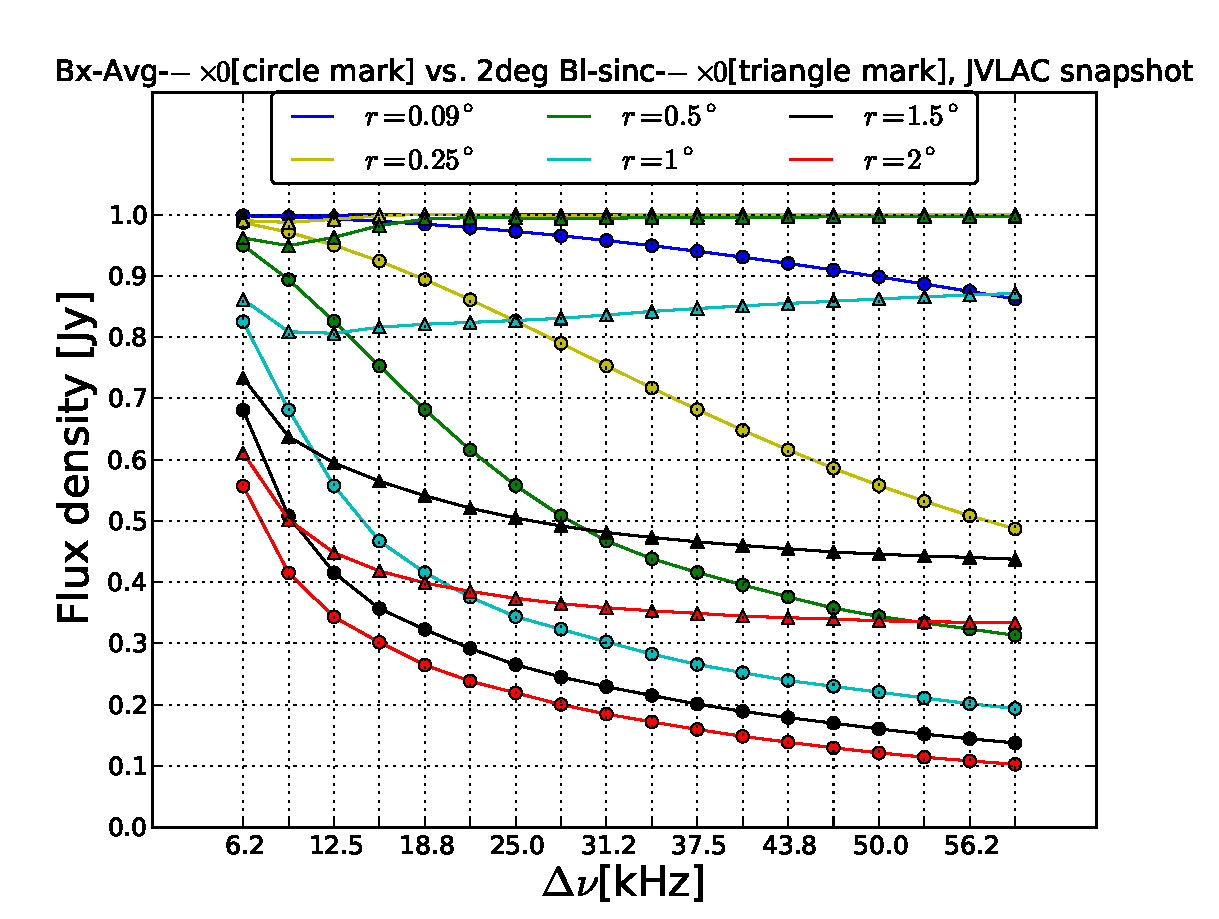
\includegraphics[width=1\textwidth]{./Figures/max-integ-freq-bessel-w1x1-fov2.pdf}
        \caption{Response to a 1Jy source at different positions, as a function of bandwidth with $2^{\circ}$ frequency Bessel first kind 
of 
  order zero filter.}
        \label{fig:max-integ-freq-bessel-w1x1-fov2}
        \end{minipage}
  \hspace{1cm}
  \begin{minipage}{0.38\linewidth}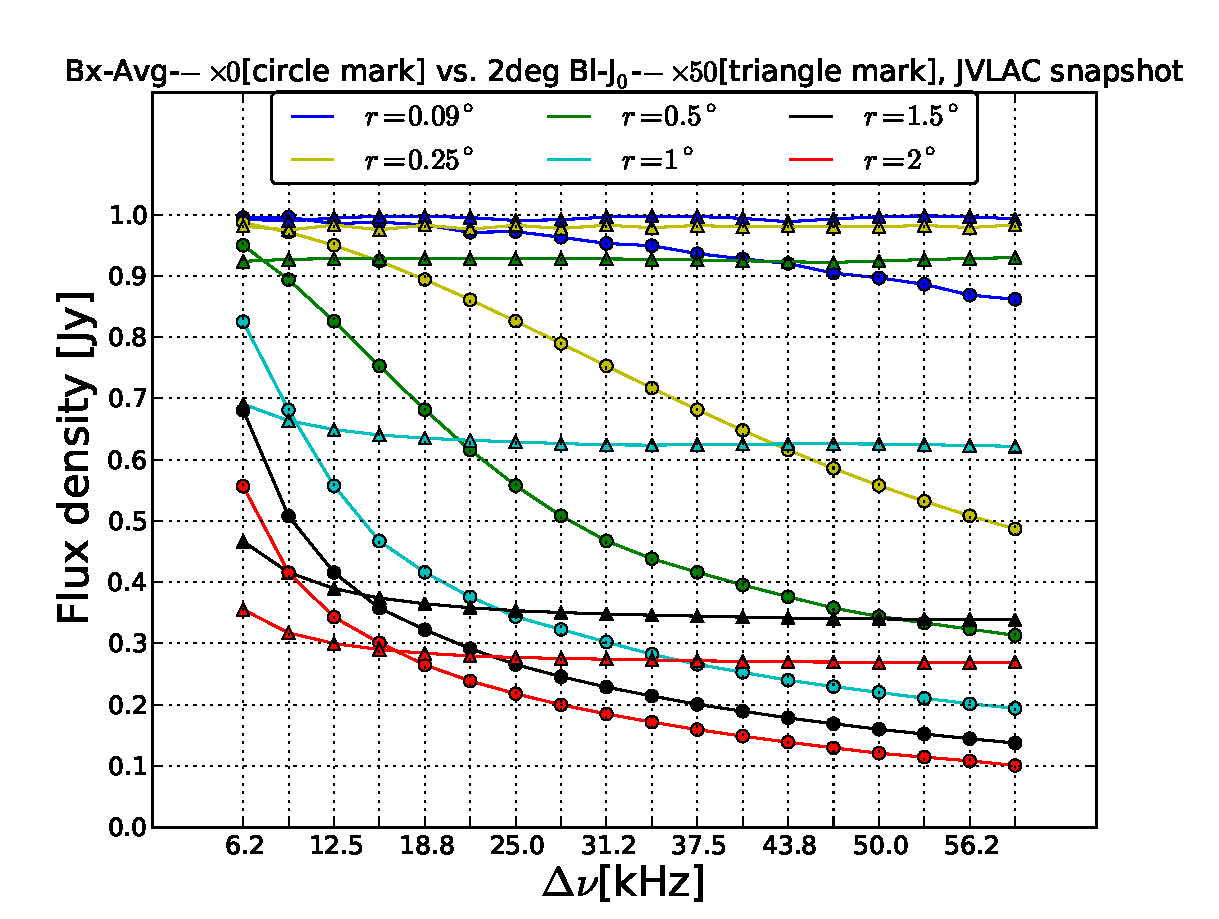
\includegraphics[width=1\textwidth]{./Figures/max-integ-freq-bessel-w1x50-fov2.pdf}
        \caption{Response to a 1Jy source at different positions, as a function of bandwidth with $2^{\circ}$ frequency overlap Bessel 
first kind filter of order zero filter.}
        \label{fig:max-integ-freq-bessel-w1x50-fov2}
        \end{minipage}
\begin{minipage}{0.38\linewidth}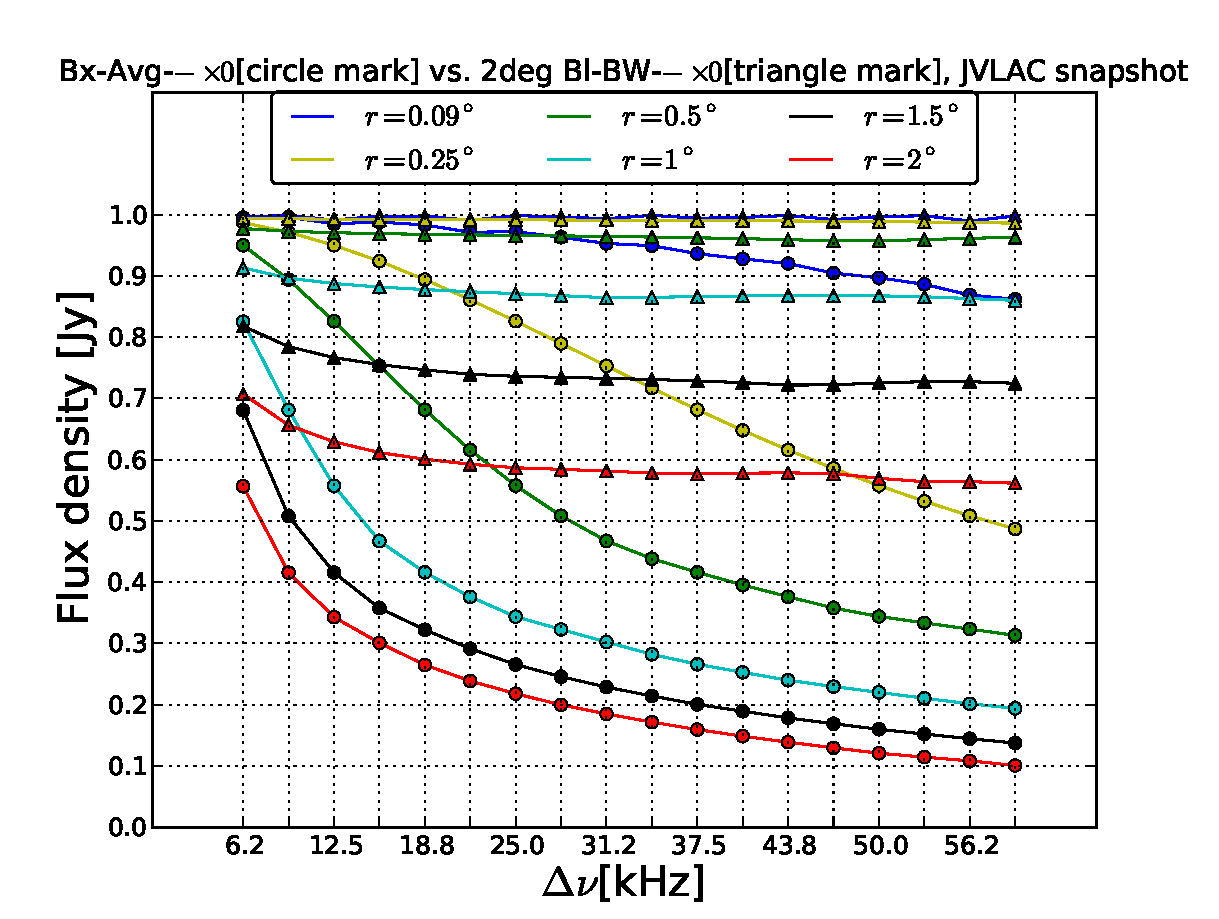
\includegraphics[width=1\textwidth]{./Figures/max-integ-freq-butter-w1x1-fov2.pdf}
      \caption{Response to a 1Jy source at different positions, as a function of bandwidth with $2^{\circ}$ frequency Butterwordth filter.}
      \label{fig:max-integ-freq-butter-w1x1-fov2}
      \end{minipage}
\hspace{1cm}
\begin{minipage}{0.38\linewidth}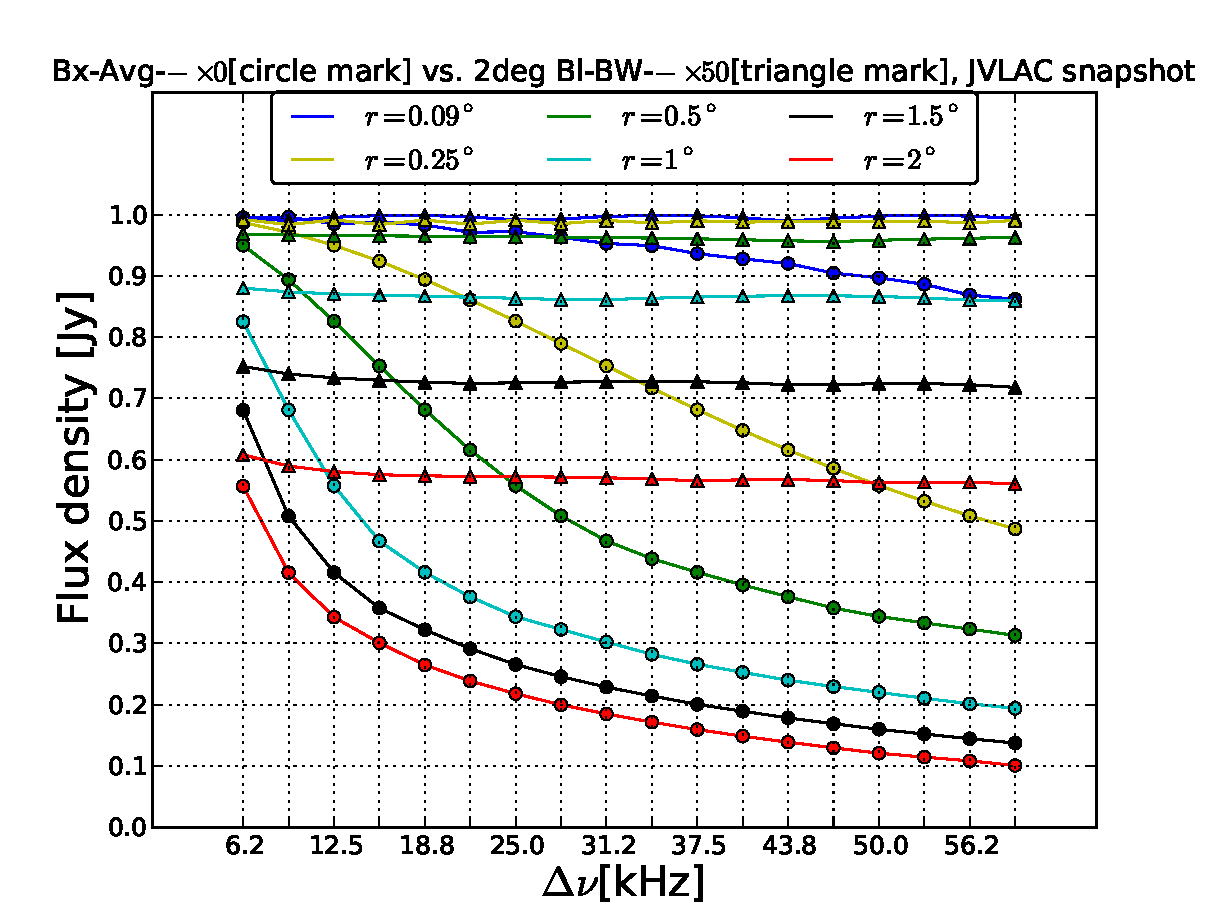
\includegraphics[width=1\textwidth]{./Figures/max-integ-freq-butter-w1x50-fov2.pdf}
      \caption{Response to a 1Jy source at different positions, as a function of bandwidth with $2^{\circ}$ frequency overlap Butterwordth 
filter.}
      \label{fig:max-integ-freq-butter-w1x50-fov2}
      \end{minipage}
\end{figure*}
\begin{figure*}
% *********************** Scripts that created these plots ***********************************
%plot.plot(wind1='/home/atemkeng/TempleFull/DATA/Maxtime-bessel-fov2-window/',title1=r'Avg[circle mark] vs. Bl-J$_0$-W$1\times 1$ [triangle 
	    %mark], FoV=2$^\circ$',xlabel=r'$\Delta t$[s]')
  \centering
\begin{minipage}{0.38\linewidth}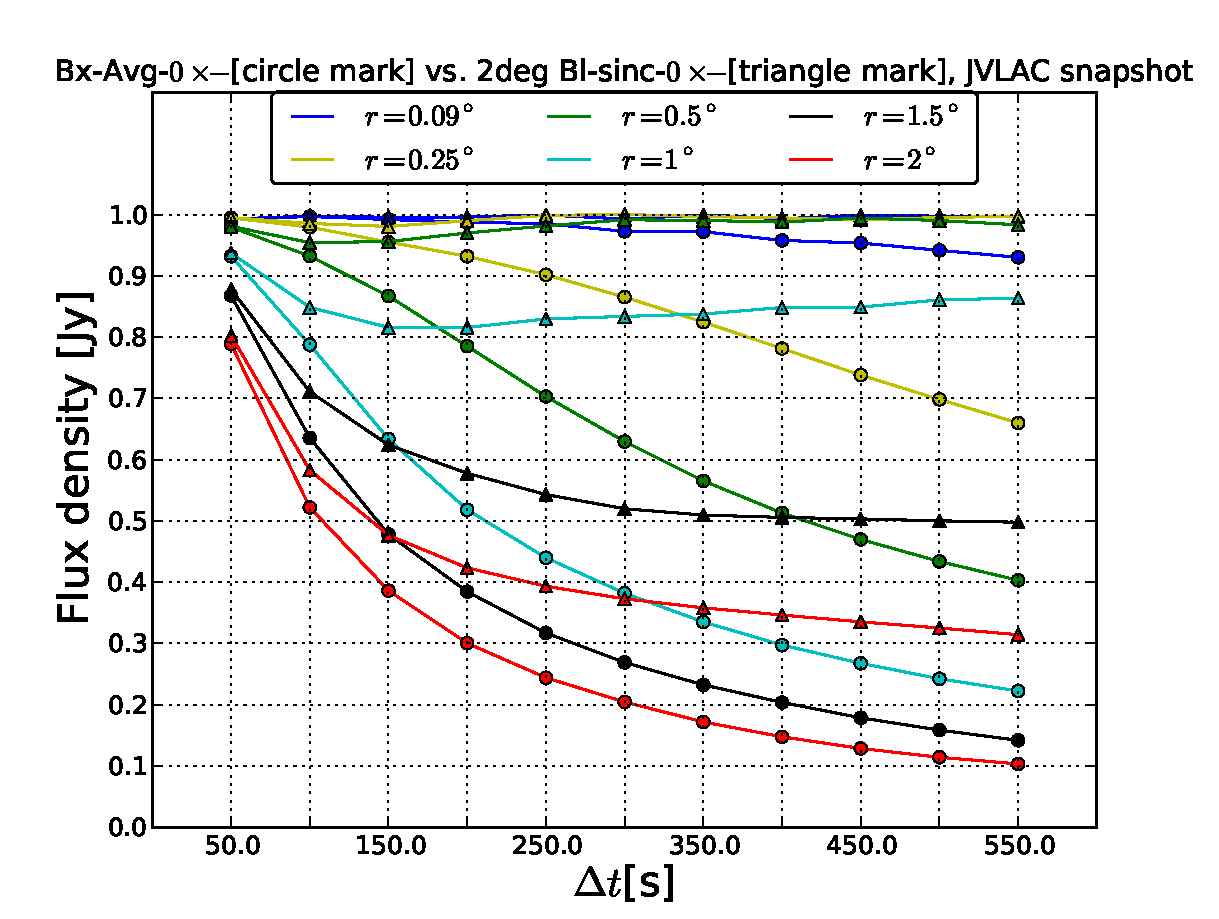
\includegraphics[width=1.\textwidth]{./Figures/max-integ-time-sinc-w1x1-fov2.pdf}
	\caption{Response to a 1Jy source at different positions, as a function of integration time with $2^{\circ}$ time sinc filter.}
	\label{fig:max-integ-time-sinc-w1x1-fov2}
	\end{minipage} \hspace{1cm}
\begin{minipage}{0.38\linewidth}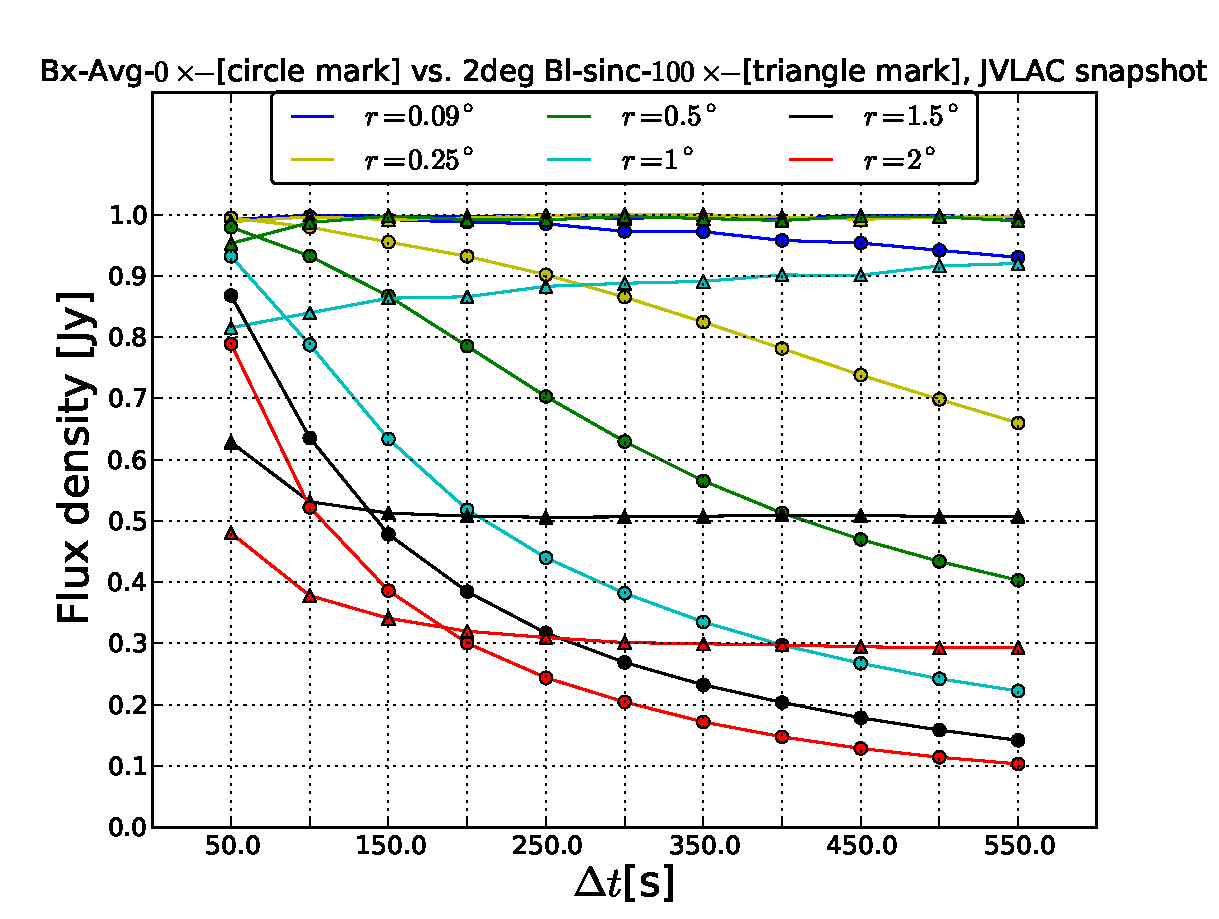
\includegraphics[width=1.\textwidth]{./Figures/max-integ-time-sinc-w100x1-fov2.pdf}
        \caption{Response to a 1Jy source at different positions, as a function of integration time with $2^{\circ}$ time overlap sinc 
filter.}
      \label{fig:max-integ-time-sinc-w100x1-fov2}
      \end{minipage}\\
\begin{minipage}{0.38\linewidth}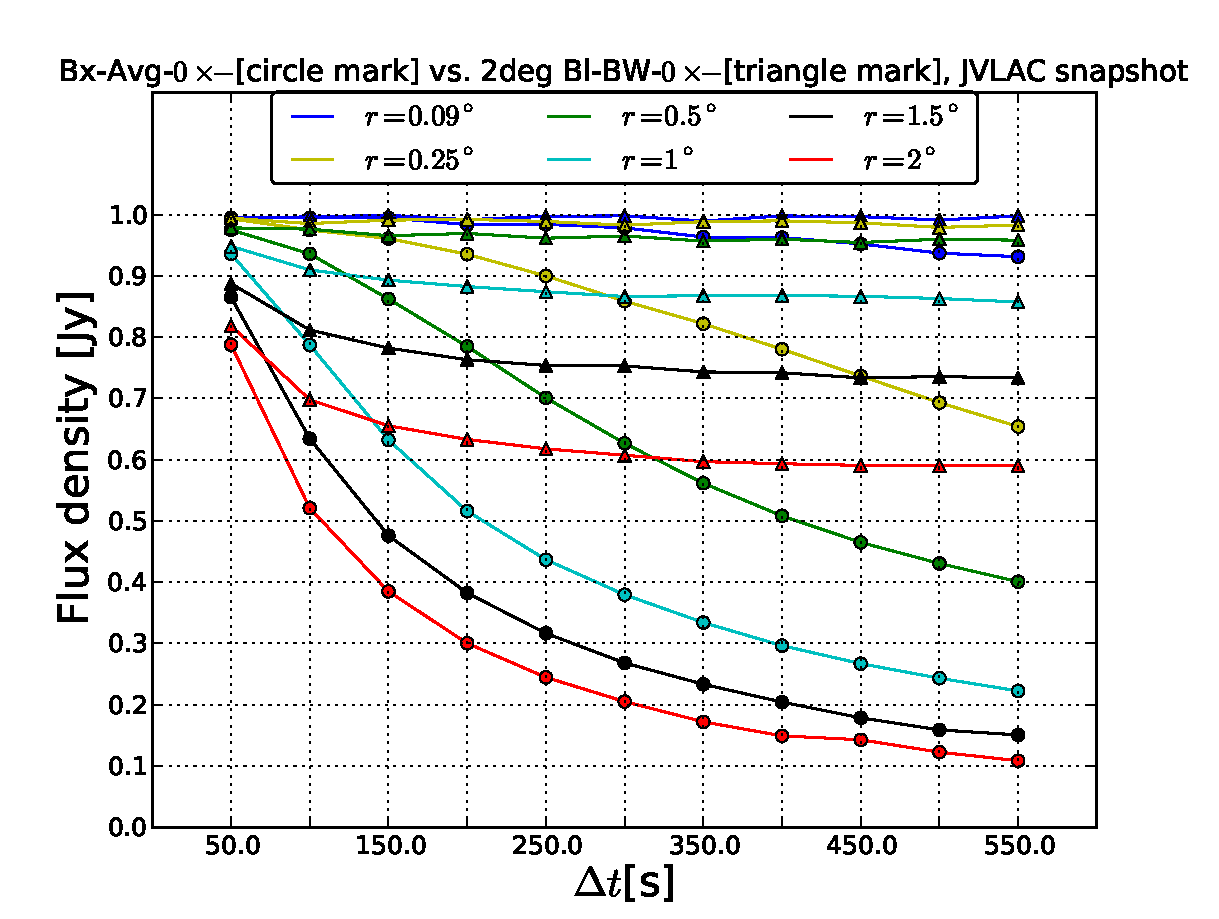
\includegraphics[width=1\textwidth]{./Figures/max-integ-time-bessel-w1x1-fov2.pdf}
    \caption{Response to a 1Jy source at different positions, as a function of integration time with $2^{\circ}$ time Bessel first kind of 
order zero
filter.}
    \label{fig:max-integ-time-bessel-w1x1-fov2}
    \end{minipage} 
 \hspace{1cm}
\begin{minipage}{0.38\linewidth}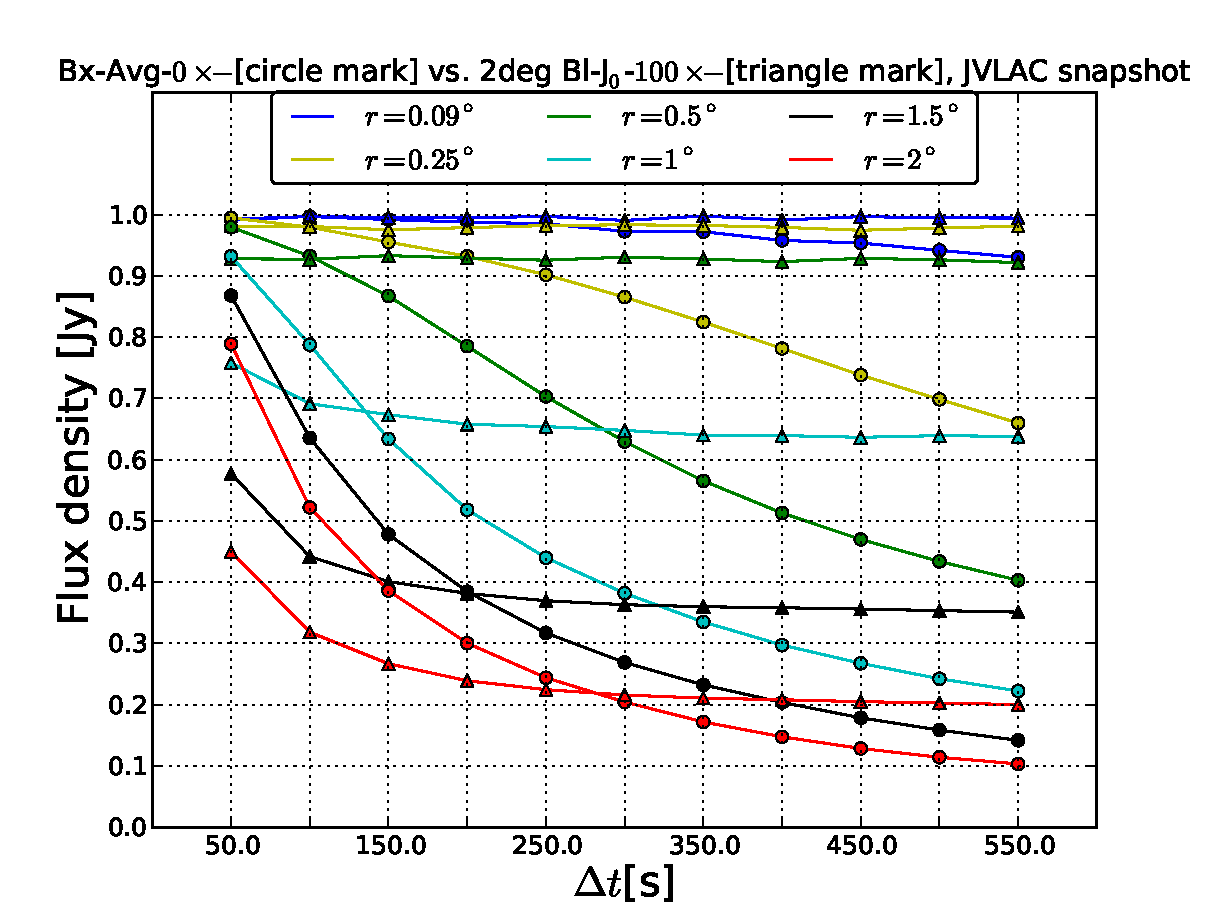
\includegraphics[width=1\textwidth]{./Figures/max-integ-time-bessel-w100x1-fov2.pdf}
    \caption{Response to a 1Jy source at different positions, as a function of integration time with $2^{\circ}$ time overlap 
      Bessel first kind of order zero filter.}
    \label{fig:max-integ-time-bessel-w100x1-fov2}\end{minipage}\\
\begin{minipage}{0.38\linewidth}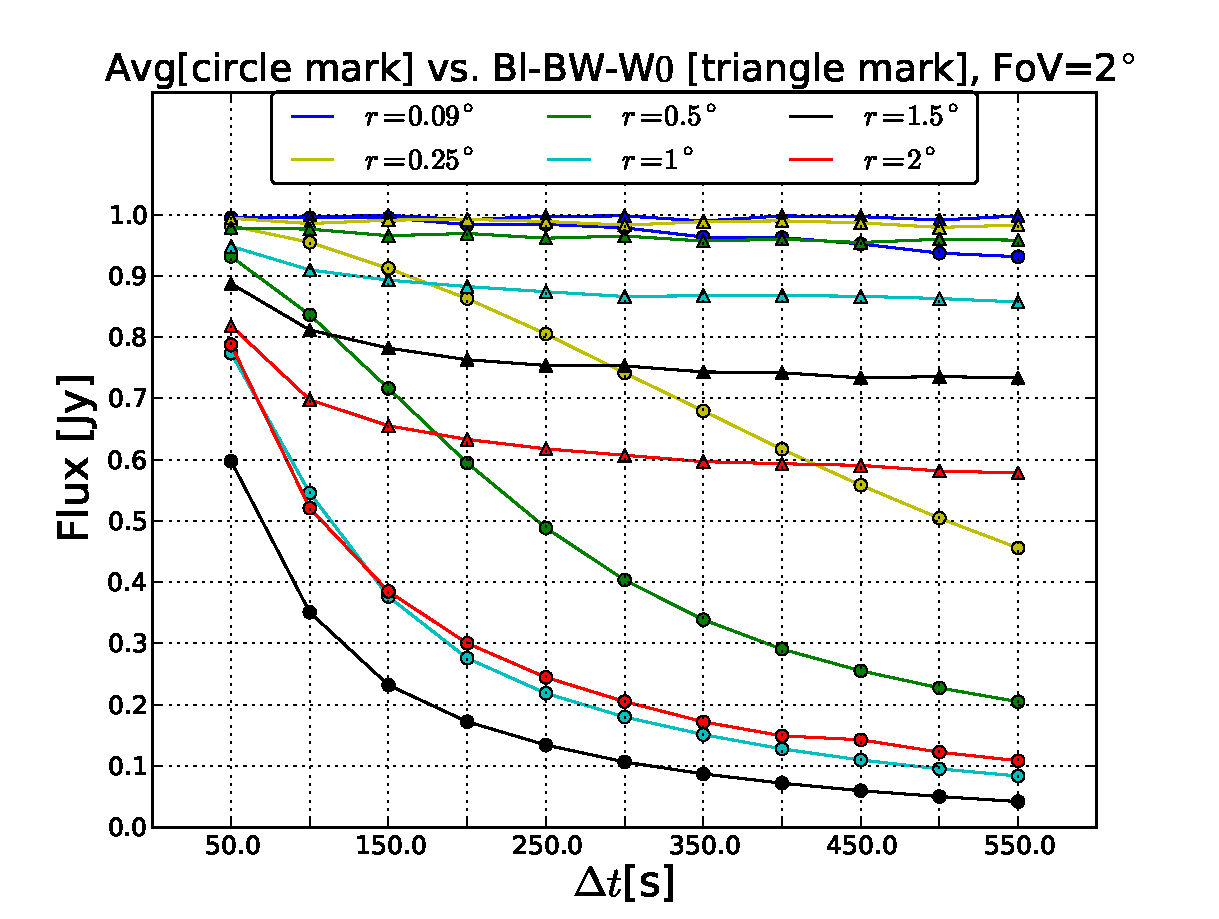
\includegraphics[width=1\textwidth]{./Figures/max-integ-time-butter-w1x1-fov2.pdf}
    \caption{Response to a 1Jy source at different positions, as a function of integration time with $2^{\circ}$ time Butterwordth 
filter.}
    \label{fig:max-integ-time-butter-w1x1-fov2}
    \end{minipage} 
 \hspace{1cm}
\begin{minipage}{0.38\linewidth}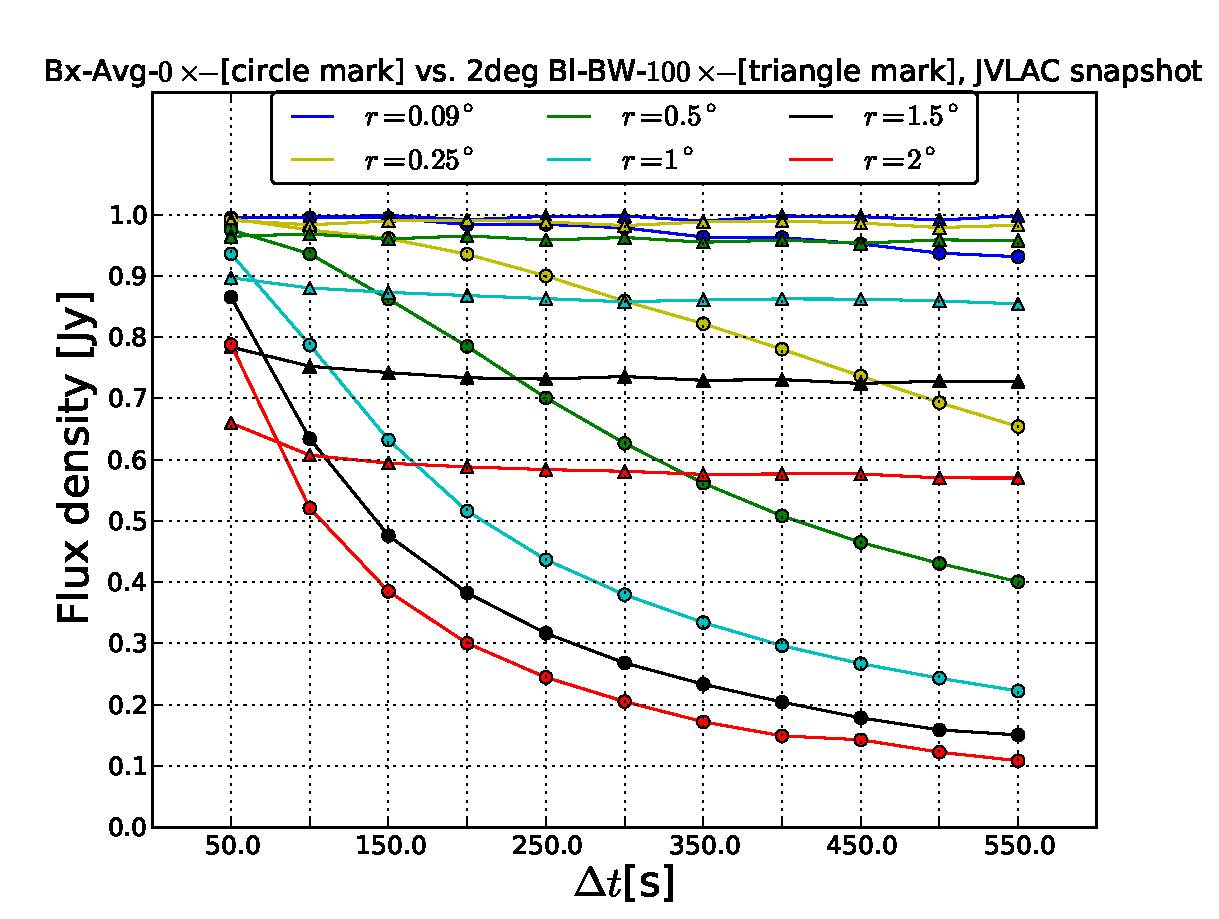
\includegraphics[width=1\textwidth]{./Figures/max-integ-time-butter-w100x1-fov2.pdf}
    \caption{Response to a 1Jy source at different positions, as a function of integration time with $2^{\circ}$ time overlap 
      Butterwordth filter.}
    \label{fig:max-integ-time-butter-w100x1-fov2}\end{minipage}   
\end{figure*}
\begin{figure*}
  \centering
\begin{minipage}{0.38\linewidth}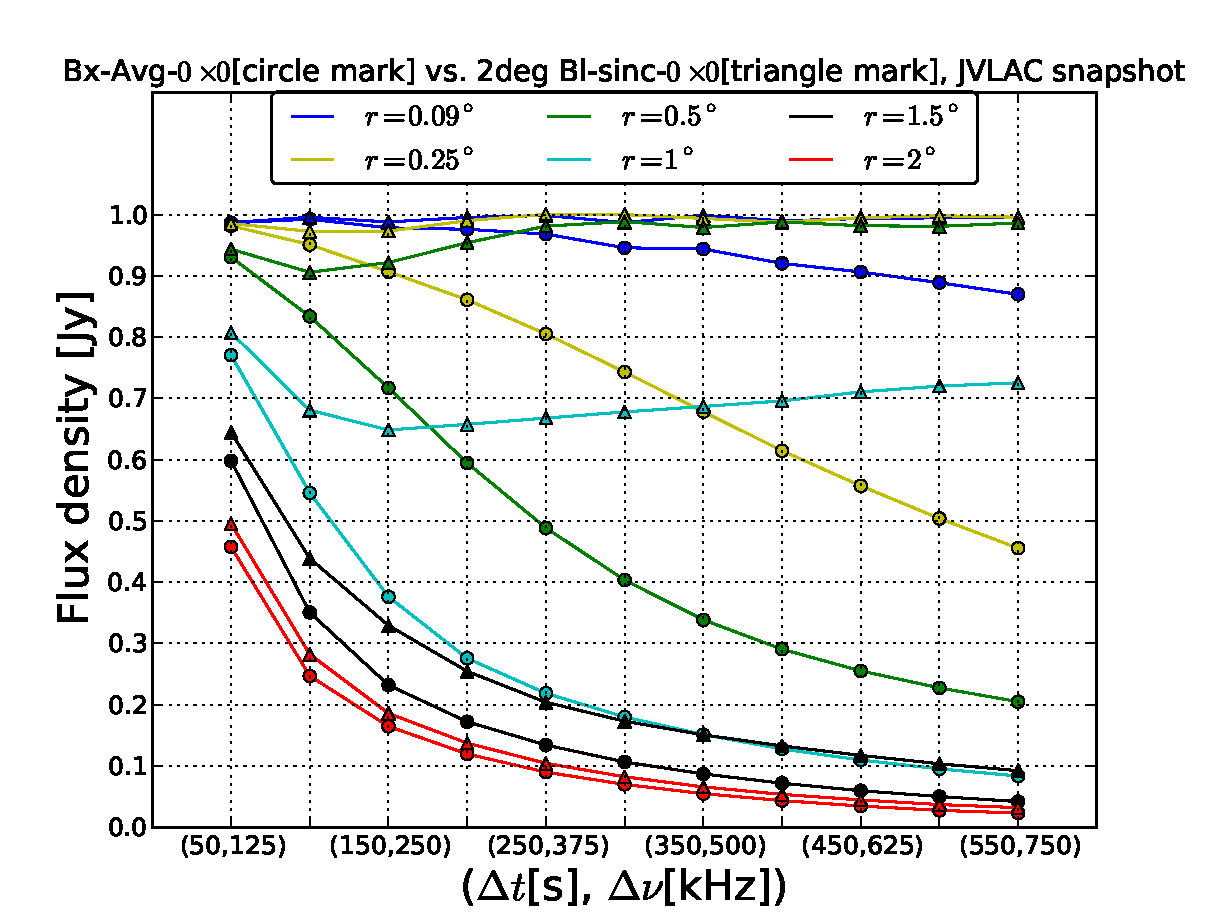
\includegraphics[width=1\textwidth]{./Figures/max-integ-timefreq-sinc-w1x1-fov2.pdf}
    \caption{Response to a 1Jy source at different positions, as a function of integration time and bandwidth; with $2^{\circ}$ frequency 
sinc filter.}
    \label{fig:max-integ-timefreq-sinc-w1x1-fov2}\end{minipage}
 \hspace{1cm}
\begin{minipage}{0.38\linewidth}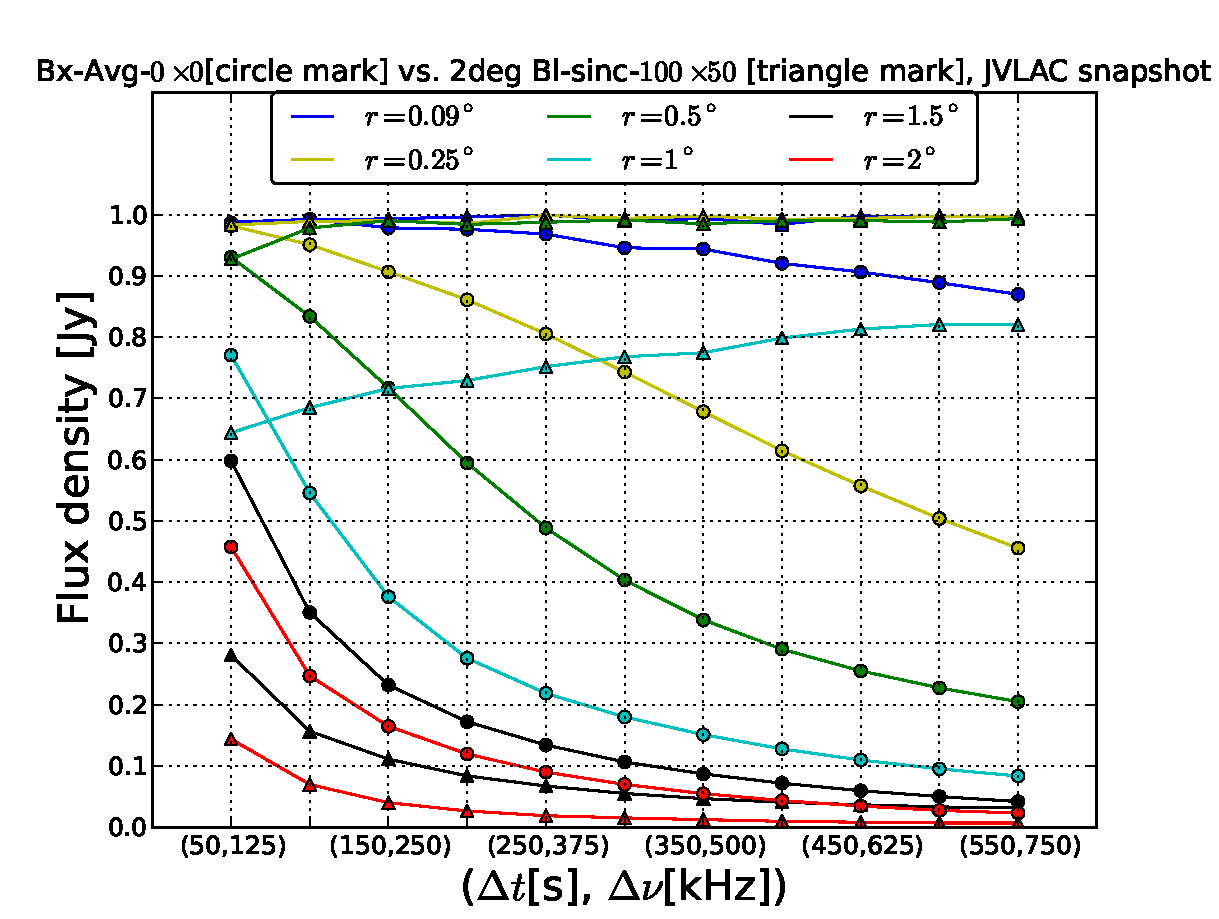
\includegraphics[width=1\textwidth]{./Figures/max-integ-timefreq-sinc-w100x50-fov2.pdf}
    \caption{Response to a 1Jy source at different positions, as a function of integration time and bandwidth; with $2^{\circ}$ frequency 
 overlap sinc filter.}
    \label{fig:max-integ-timefreq-sinc-w100x50-fov2}\end{minipage}\\
\begin{minipage}{0.38\linewidth}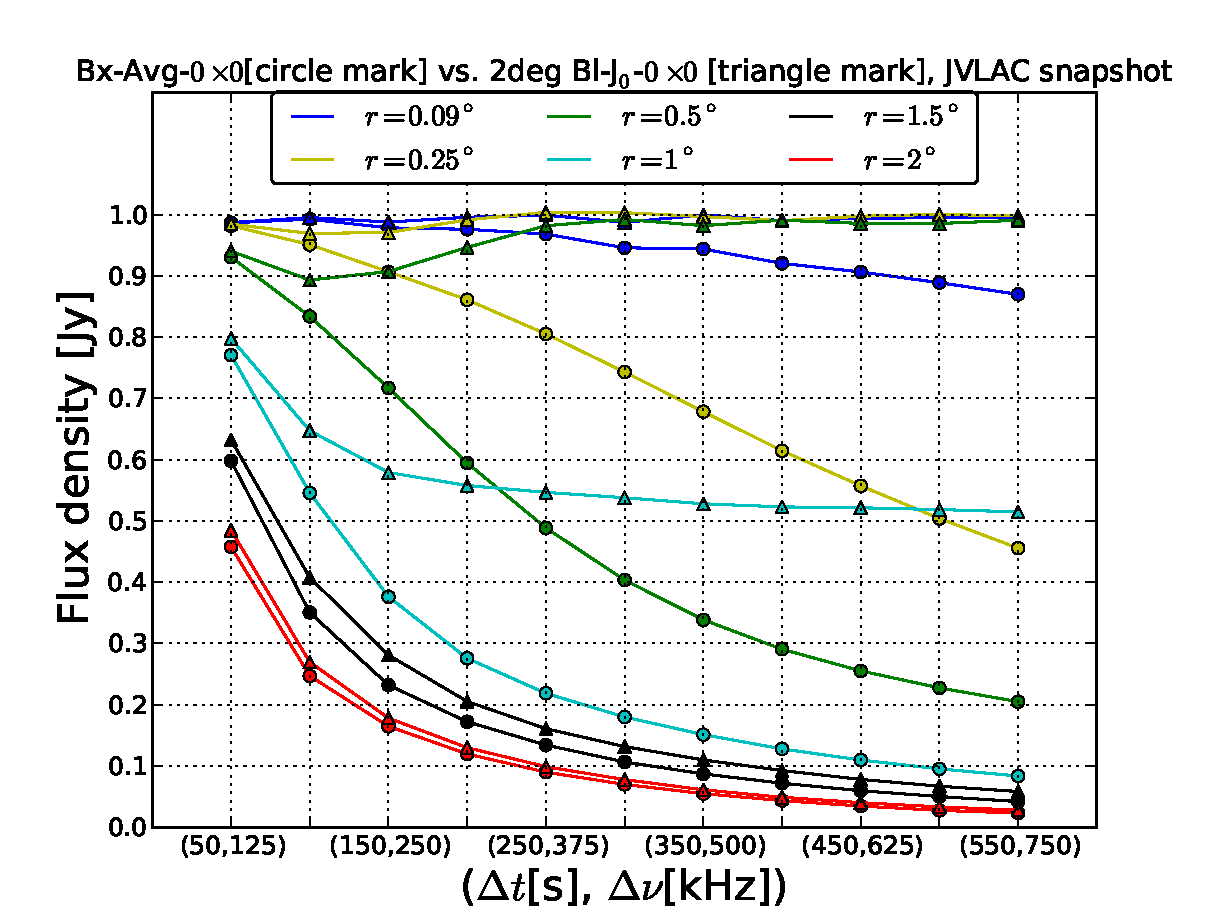
\includegraphics[width=1\textwidth]{./Figures/max-integ-timefreq-bessel-w1x1-fov2.pdf}
      \caption{Response to a 1Jy source at different positions, as a function of integration time and bandwidth, with $2^{\circ}$ frequency 
Bessel first kind of order zero filter.}
      \label{fig:max-integ-timefreq-bessel-w1x1-fov2}\end{minipage}
\hspace{1cm}
\begin{minipage}{0.38\linewidth}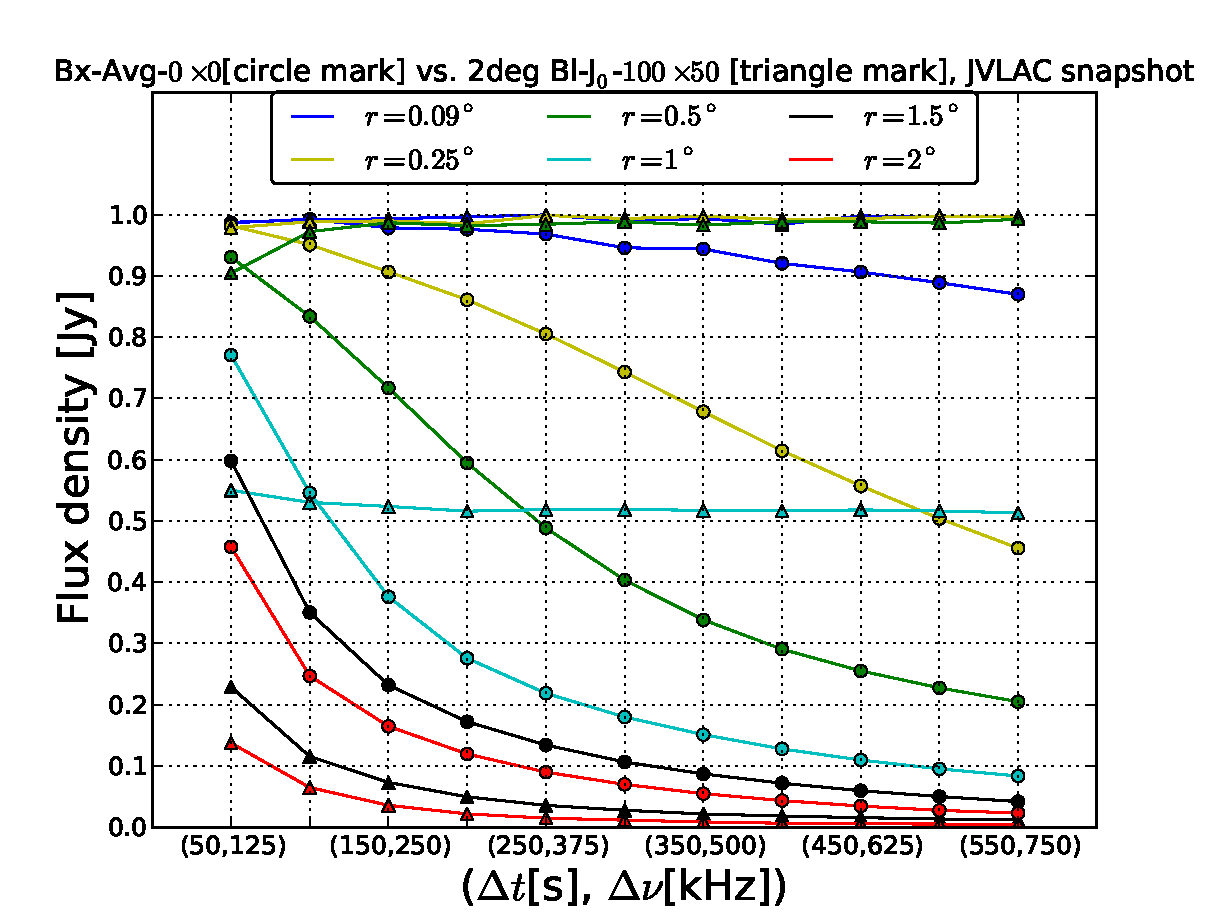
\includegraphics[width=1\textwidth]{./Figures/max-integ-timefreq-bessel-w100x50-fov2.pdf}
      \caption{Response to a 1Jy source at different positions, as a function of integration time and bandwidth, with $2^{\circ}$ frequency 
overlap Bessel first kind of order zero filter.}
  \label{fig:max-integ-timefreq-bessel-w100x50-fov2}\end{minipage}
\begin{minipage}{0.38\linewidth}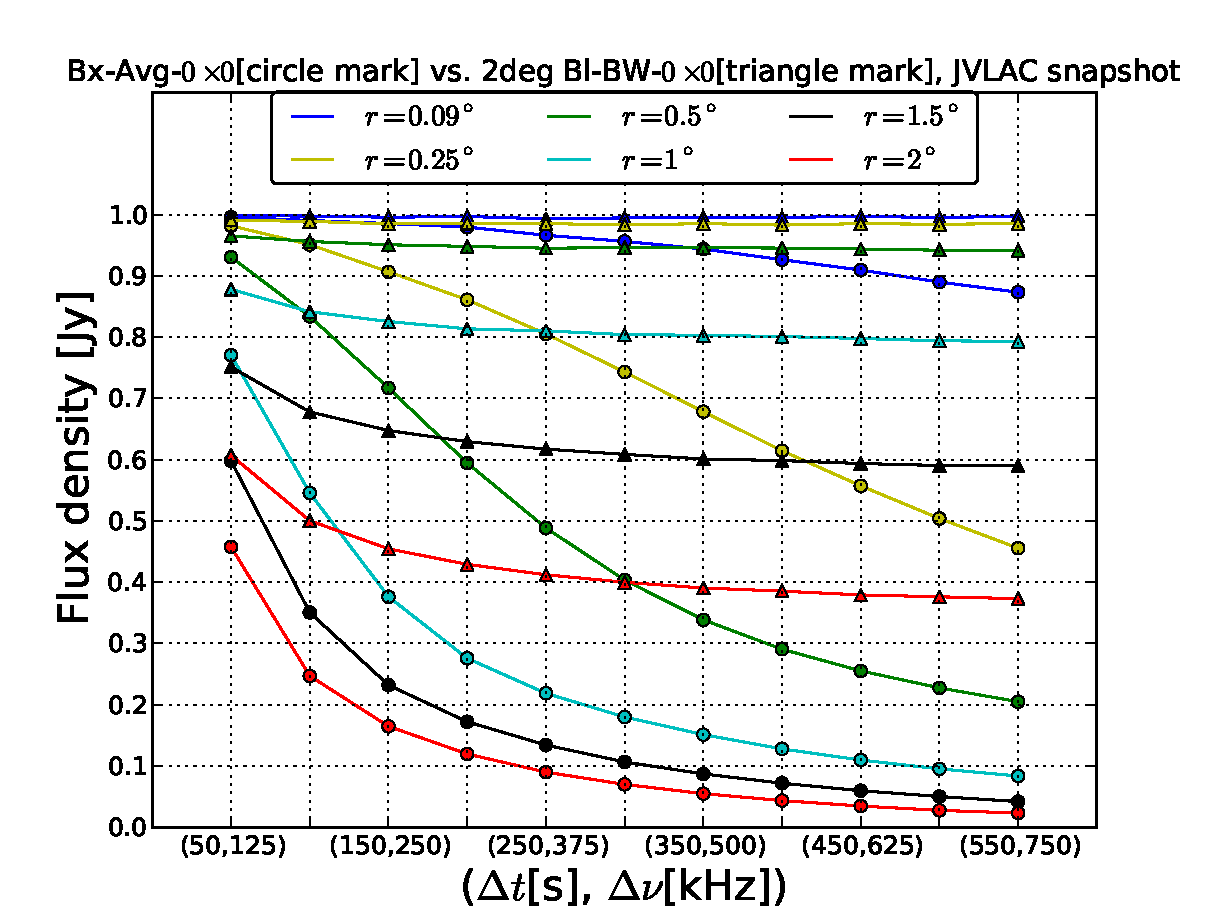
\includegraphics[width=1\textwidth]{./Figures/max-integ-timefreq-butter-w1x1-fov2.pdf}
      \caption{Response to a 1Jy source at different positions, as a function of integration time and bandwidth, with $2^{\circ}$ frequency 
Butterwordth filter.}
      \label{fig:max-integ-timefreq-butter-w1x1-fov2}\end{minipage}
\hspace{1cm}
\begin{minipage}{0.38\linewidth}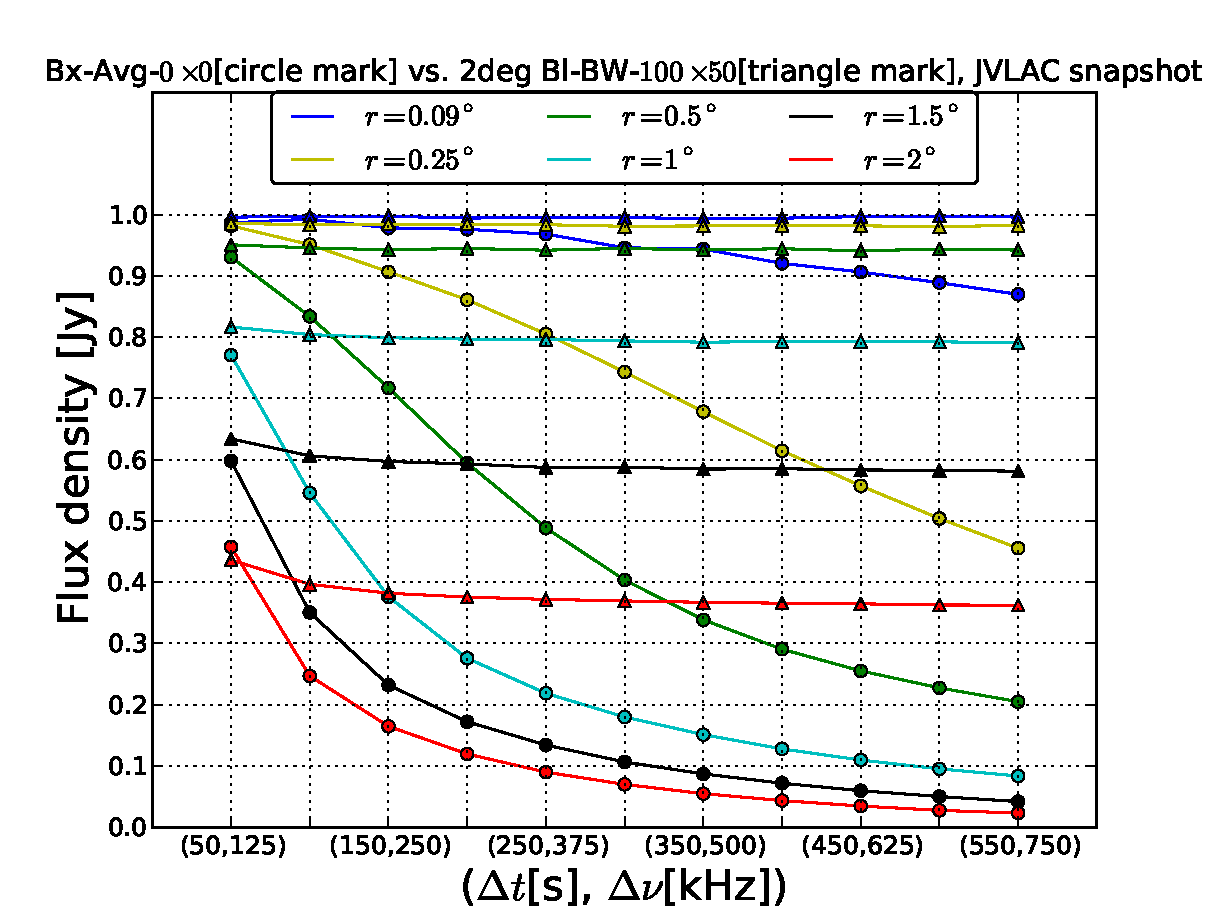
\includegraphics[width=1\textwidth]{./Figures/max-integ-timefreq-butter-w100x50-fov2.pdf}
      \caption{Response to a 1Jy source at different positions, as a function of integration time and bandwidth, with $2^{\circ}$ frequency 
overlap Butterwordth filter.}
  \label{fig:max-integ-timefreq-butter-w100x50-fov2}\end{minipage}
\end{figure*}
\section{Conclusions}
The goal of this paper was threefold. The original motivation behind the work presented in this

paper was to **** windowing functions***\\
The second objective  was to study ****first algorithm data compression***\\
The final objective was to ****second algorithm data compression and out field suppression*** \\
Drawback and futures works*** drawback and futures works*****
\section*{Acknowledgements}
The research  made use of  MeqTrees software system designed to implement numerical models for third-generation calibration (3GC) 
 Python Extensions for Interferometry and Python. The research has been supported by the South Africa National Research Foundation.
\bibliographystyle{mn2e}
\bibliography{m_paper}
\appendix
\section[]{Derivation of complex matrices}
\label{app:complexmatrices}
The complex matrices used in section \ref{sec:imaging} are explicitly derived in this appendix. In Eq.\ref{eqbb:linear}, the matrices
$\mathbf{C}_{(t,\nu)}^{block}$ and $\mathbf{W}_{pq,(t,\nu)}^{block}$ are blocks diagonals  both of size $(4n_t n_{\nu})\times(4n_t 
n_{\nu})$ explicitly expressed as follow:
\begin{equation*}
\mathbf{C}_{(t,\nu)}^{block}=
  \begin{bmatrix}
    \mathbf{c}_{(t,\nu)} & 0 & 0 & 0\\
    0 &  \mathbf{c}_{(t,\nu)} &0 & 0 \\
    0 & 0 & \mathbf{c}_{(t,\nu)} & 0\\
      0 & 0 & 0 & \mathbf{c}_{(t,\nu)}\\
  \end{bmatrix}
\end{equation*}
\begin{equation*}
\mathbf{W}_{pq,(t,\nu)}^{block}=
  \begin{bmatrix}
    \mathbf{W}_{pq,(t,\nu)}& 0 & 0 & 0\\
    0 &  \mathbf{W}_{pq,(t,\nu)} &0 & 0 \\
    0 & 0 & \mathbf{W}_{pq,(t,\nu)} & 0\\
      0 & 0 & 0 & \mathbf{W}_{pq,(t,\nu)}\\
  \end{bmatrix}
\end{equation*}
In Eq.\ref{eq2:block}, the matrices $\mathbf{C}_{pq,(t,\nu)}^{block,n_{block}}$ and 
$\mathbf{W}_{pq,(t,\nu)}^{block,n_{block}}$ are blocks diagonals both of size $(4N_v^{pq}n_t n_{\nu})\times (4N_v^{pq}n_t n_{\nu})$, and 
the sampled visibilities $\mathbf{V}_{pq,(t,\nu)}^{samp,nblock}$ is a one row matrix of size $(N_v^{pq}4 n_t n_{\nu})\times (4 n_t 
n_{\nu})$ 
made of $\textbf{V}_{pq,(t,\nu)}^{samp}$. These matrices are explicitly expressed as follow:
\begin{equation*}
\mathbf{C}_{pq,(t,\nu)}^{block,n_{block}}=
  \begin{bmatrix}
    \mathbf{C}_{pq,(t,\nu)}^{block} &\dots & 0 & \dots & 0\\
    \vdots & \vdots & \vdots & \vdots & \vdots\\
    0 & \dots& \mathbf{C}_{pq,(t,\nu)}^{block} &\dots & 0\\
    \vdots & \vdots & \vdots & \vdots & \vdots \\
    0 & \dots& 0 &\dots & \mathbf{C}_{pq,(t,\nu)}^{block}\\
  \end{bmatrix}
\end{equation*}
\begin{equation*}
\mathbf{W}_{pq,(t,\nu)}^{block,n_{block}}=
  \begin{bmatrix}
    \mathbf{W}_{pq,(t,\nu)}^{block} &\dots & 0 & \dots & 0\\
    \vdots & \vdots & \vdots & \vdots & \vdots\\
    0 & \dots& \mathbf{W}_{pq,(t,\nu)}^{block} &\dots & 0\\
    \vdots & \vdots & \vdots & \vdots & \vdots \\
    0 & \dots& 0 &\dots & \mathbf{W}_{pq,(t,\nu)}^{block}\\
  \end{bmatrix}
\end{equation*}
\begin{eqnarray*}
\mathbf{V}_{pq,(t,\nu)}^{samp,n_{block}}&=&\Big(\mathbf{V}_{pq,(t,\nu)}^{samp,1},\dots, \mathbf{V}_{pq,(t,\nu)}^{samp,k}, \dots,
\mathbf{V}_{pq,(t,\nu)}^{samp,N^{pq}_v}\Big)^{\dagger}. 
\end{eqnarray*}
In Eq.\ref{eq:noise}, the matrix $\mathbf{B}$ of size $(N_v 4 n_t n_{\nu})\times (4 n_t n_{\nu})$ is defined as follow:
\begin{equation*}
\mathbf{B}_{}=
  \begin{bmatrix}
    \mathbf{C}_{01,(t,\nu)}^{block,n_{block}}\cdot \mathbf{W}_{01,(t,\nu)}^{block,n_{block}}\\
    \vdots\\
    \mathbf{C}_{ik,(t,\nu)}^{block,n_{block}}\cdot \mathbf{W}_{ik,(t,\nu)}^{block,n_{block}}\\
    \vdots \\
    \mathbf{C}_{jl,(t,\nu)}^{block,n_{block}}\cdot \mathbf{W}_{jl,(t,\nu)}^{block,n_{block}}
  \end{bmatrix}
\end{equation*}
% \section[]{Sky tapering function with averaging}
% \label{label:similarimaging}
% The measured sky intensity of the array is derived from the inverse Fourier transform of the sum of the sample visibilities 
% measured at each baseline.
% \begin{eqnarray*}
%  \mathcal{I}^{D}_{l,m}&=& \mathcal{F}^{-1}\Bigg\{\sum_{pq} c_{pq,(t,\nu)}\cdot\Big(\Pi_{pq}\circ V_{pq}^{samp}\Big)_{(t,\nu)}\Bigg\}\\
% 		      &=&\sum_{pq} \mathcal{F}^{-1}\{c_{pq,(t,\nu)}\}\circ \Big(\mathcal{F}^{-1}\{\Pi_{pq,(t,\nu)}\}\cdot 
% \mathcal{F}^{-1}\{V_{pq,(t,\nu)}^{samp}\}\Big)
% \end{eqnarray*}
% \begin{eqnarray*}	     
% \mathcal{I}^{D}_{l,m}&=&\sum_{pq}\mathcal{F}^{-1}\{\Pi_{pq,(t,\nu)}\}\cdot\bigg(\mathcal{F}^{-1}\{S_{pq}\cdot V_{pq,(t,\nu)}\}
% \bigg)
% \end{eqnarray*}
% recall from section \ref{sec:AvgCon} that $S_{pq}$ is the sampling function of the baseline $pq$ and $\Pi_{pq,(t,\nu)}$ is the 
% boxcar window.  This can be re-written as
% \begin{eqnarray*}	     
% \mathcal{I}^{D}_{l,m}&=&\sum_{pq} \mathcal{R}_{pq} \cdot\bigg(\mathcal{B}_{pq}\circ \mathcal{I}^{sky}_{l,m}\bigg)
% \end{eqnarray*}
% If all baselines are seen the same sky, then we can write:
% \begin{eqnarray*}	     
% \mathcal{I}^{D}_{l,m}&=&\mathcal{R}_{}\cdot\Bigg(\bigg(\sum_{pq}\mathcal{B}_{pq}\bigg)\circ \mathcal{I}^{sky}_{l,m}\Bigg)
% \end{eqnarray*}
% Here, $\mathcal{B}_{pq}$ is the point spread function for the baseline $pq$ and $\mathcal{R}_{pq}= \mathcal{R}$ is the sky taper, where 
% $\mathcal{R}_{}=sinc$.\\
% \\
\bsp
\label{lastpage}
\end{document}
